%&preamble.main

% NOTE ciclo di compilazione
% arara: pdflatex: { shell: yes, draft: yes }
% arara: pdflatex: { shell: yes, synctex: yes }
%! arara: latexmk:  { clean: partial }
\begin{document}

\frontmatter

    % NOTE nessun contatore delle pagine
	\pagenumbering{gobble}
	\maketitle

\mainmatter

	% NOTE disabilita la protrusion localmente
	\microtypesetup{protrusion = false}

	% NOTE % sections + subsections
	\setcounter{tocdepth}{2}
	\tableofcontents

	\listoffigures

	% \listoftables

	% TODO risolvere questo problema
	% \listoftheorems[ignoreall, show={theorem, definition}] % NOTE si sovrascrivono
	\renewcommand{\thmtformatoptarg}[1]{ -- #1}
	\renewcommand{\listtheoremname}{Elenco dei teoremi}
	\listoftheorems[ignoreall, show={theorem}]
	% \listoftheorems[ignoreall, show={definition}]
	% \listoftheorems[ignoreall, show={note}]

	% TODO risolvere questo problema
	% \listofalgorithms % NOTE non stampa nulla

	% NOTE (ri)abilita la protrusion
	\microtypesetup{protrusion = true}
	\cleardoublepage

	% TODO scrivere il prologo
	% \afterpage{\blankpage}
	% \chapter*{Prologo}
	% \blankpage

	\part{Primo semestre}

	\pagenumbering{arabic}
	\pagestyle{mystyle}

	\subfile{02-analisi}
	\subfile{03-funzioni}
	\subfile{04-strutture}
	\subfile{05-alberi}
	\subfile{06-abr}
	\subfile{08-insiemi-dizionari}
	\subfile{09-grafi}
	\subfile{12-dividi}

	% \part{Secondo semestre}

	% %&../settings/preamble.main

\ifloadsubpreamble
\pagestyle{plain}
\setcounter{chapter}{10}
\fi

% arara: pdflatex: { draft: yes, synctex: no }
% arara: pdflatex: { synctex: no }
% arara: latexmk:  { clean: partial }
\begin{document}
\chapter{Scelta della struttura dati}

\begin{note}
La prima cosa da fare quando si progetta un algoritmo è capire quale sia la struttura dati adatta a risolvere quel particolare problema.
\end{note}

\section{Cammini minimi, sorgente singola}

\subsection{Problema dei cammini minimi}

\begin{definition}[Costo del cammino]
Dato un cammino \(p = \angleled{v_1, v_2, \ldots, v_k}\) con \(k > 1\), il \emph{costo del cammino} (\foreign{weight of the path}) è dato da
\begin{equation*}
w(p) = \sum_{i=2}^k w(v_{i-1}, v_i)
\end{equation*}
\end{definition}
Ossia dalla somma dei singoli pesi dei lati che compongono il percorso.

\paragraph{Definizione del problema}
Dati in input un grafo orientato \(G = (V, E)\), un nodo sorgente \(s\) ed una funzione di peso \(w \colon E \to R\) (che associa ad ogni arco un numero reale che rappresenta il peso).

Trovare un cammino da \(s\) ad \(u\), per ogni nodo \(u \in V\), il cui costo sia minimo, ovvero più piccolo o uguale al costo di qualunque altro cammino da \(s\) a \(u\).

\begin{note}
Non ci limitiamo a trovare un solo percorso, ma tutti i cammini da un nodo a tutti gli altri nodi.
\end{note}

\paragraph{Panoramica sul problema}

Per risolvere il problema del cammino minimo fra una coppia di vertici, si risolve il problema di cammini minimi da sorgente unica (si trovano tutti i cammini che partono da un nodo) e si estrae il cammino richiesto.
Per quanto riguarda il \emph{caso pessimo} non si conoscono algoritmi che abbiamo tempo di esecuzione migliore.

In alcuni casi gli archi possono avere peso negativo. Questo influisce sul problema (se è ben definito oppure no) e sulla soluzione (in assenza di archi negativi si \textcolor{red}{(possono?)} devono utilizzare tecniche diverse).

Nell'algoritmo di Dijkstra si suppone che tutti gli archi abbiano peso positivo, mentre nell'algoritmo di Bellman-Ford gli archi possono avere peso negativo, ma non possono esistere cicli di peso negativo.

\begin{note}
In generale possiamo ammettere pesi negativi, ma non cicli negativi.
\end{note}

\paragraph{Considerazioni sui cicli}
Se esiste un ciclo di peso negativo raggiungibile dalla sorgente, non esistono cammini finiti di peso minimo;
per qualunque cammino, basterà passare per un ciclo negativo più volte per ottenere un ciclo di costo inferiore.

Ovviamente, in un cammino minimo \emph{non è possibile la presenza di un ciclo di peso positivo}.
Mentre i cicli di peso nullo possono essere banalmente eliminati dal cammino minimo, in quanto inutili e ridondanti.

\subsection{Sottostruttura ottima}

Nota che due cammini minimi possono avere un tratto in comune, ma non possono convergere in un nodo comune \(B\) dopo aver percorso un tratto iniziale distinto.

\begin{figure}[H]\centering
	\begin{subfigure}[t]{.5\linewidth}\centering
		\includestandalone[mode=image]{walk-common-part}
		\caption{Due cammini minimi che hanno un tratto in comune a partire dal nodo \(B\)}%
		\label{fig:walk-common-part}
	\end{subfigure}%
	\begin{subfigure}[t]{.5\linewidth}\centering
		\includestandalone[mode=image]{walk-shared-node}
		\caption{Due cammini che convergono in un nodo comune \(B\) dopo aver percorso un tratto iniziale distinto.}%
		\label{fig:walk-shared-node}
	\end{subfigure}
	\caption{La figura~\ref{fig:walk-common-part} è una condizione ammissibile, mentre~\ref{fig:walk-shared-node} non lo è.}%
	\label{fig:sottostruttura-ottima}
\end{figure}

\begin{definition}[Albero dei cammini minimi]
L'albero dei cammini minimi è un albero di copertura radicato in \(s\) avente un cammino da \(s\) a tutti i nodi raggiungibili da \(s\).
\end{definition}

\begin{note}
Non confonderlo con gli alberi di copertura di peso minimo.
\end{note}

% NOTE è stato rimosso nelle nuove trasparenze?
% \begin{definition}[Albero di copertura, \foreign{spanning tree}]
% Dato un grafo \(G = (V, E)\) non orientato e connesso, un albero di copertura \(G\) è un sottografo di \(T = (V, E_T)\) tal che:
% \begin{itemize}
% 	\item T è un albero;
% 	\item \(E_T \subseteq E\);
% 	\item \(T\) contiene tutti i vertici di \(G\).
% \end{itemize}
% \end{definition}

\paragraph{Soluzione ammissibile}
Una soluzione \emph{ammissibile} può essere descritta da un \emph{albero di copertura \(T\)} radicato in \(s\) e da un \emph{vettore delle distanze \(d\)}, i cui valori \(d[u]\) rappresentano il costo del cammino da \(s\) a \(u\) in \(T\).

\begin{figure}[H]\centering
	\begin{subfigure}[b]{.5\linewidth}\centering
		\includestandalone[mode=image]{shortestPath-admittable}
		\caption{Soluzione ammissibile (albero di peso minimo)}%
		\label{fig:soluzione-ammissibile}
	\end{subfigure}%
	\begin{subfigure}[b]{.5\linewidth}\centering
		\includestandalone[mode=image]{shortestPath-optimal}
		\caption{Soluzione ottima (albero dei cammini minimi)}%
		\label{fig:soluzione-ottima}
	\end{subfigure}
	\caption{Nota la differenza fra i due alberi: a sinistra l'albero di \emph{peso minimo} che rappresenta una soluzione ammissibile, ma non ottima, mentre a destra l'albero dei cammini minimi, ossia l'insieme dei percorsi che minimizzano il peso fra il nodo sorgente e tutti gli altri nodi, il quale rappresenta la soluzione ottima.}
\end{figure}

\begin{note}
In questo problema devo trovare i percorsi che minimizzano il peso fra un nodo e tutti gli altri nodi, e \textbf{non}, come sembra spontaneo fare, l'albero che ha complessivamente peso minimo.
\end{note}

\paragraph{Rappresentazione dell'albero}
Utilizziamo la rappresentazione basata su vettore dei padri, così come abbiamo fatto con le visite in ampiezza/profondità.

\subsection{Teorema di Bellman}

\begin{theorem}[Teorema di Bellman]
Una soluzione ammissibile \(T\) è (anche) ottima se e solo se:
\begin{align*}
d[v] \bs{=} d[u] + w (u,v)			& \text{ per ogni arco }(u,v) \bs{\in T} \\
d[v] \bs{\leqslant} d[u] + w (u,v)	& \text{ per ogni arco }(u,v) \bs{\in E}
\end{align*}
\end{theorem}
\begin{proof}[Dimostrazione per assurdo (parte 1)]
Sia \(T\) una soluzione ottima.
Consideriamo un qualunque arco \((u,v) \in E\) e sia \(w (u, w)\) la sua lunghezza.

Ovviamente se \((u,v) \in T\), allora \(d[v] = d[u] + w(u,v)\).
Invece se \((u,v) \notin T\), allora poiché \(T\) è ottimo, deve risultare \(d[v] \leqslant d[u] + w(u,v)\), altrimenti esisterebbe nel grafo \(G\) un cammino da \(s\) a \(v\) più corto di quello in \(T\), che è \emph{assurdo} perché abbiamo ipotizzato che \(T\) fosse ottima.
\end{proof}

\begin{proof}[Dimostrazione per assurdo (parte 2)]
Supponiamo per assurdo che il cammino da \(s\) a \(u\) in \(T\) non sia ottimo.
Allora esiste un cammino da \(s\) a \(u\) con distanza \(d'[u]<d[u]\).
Sia \(d'[v]\) la distanza da \(s\) ad un generico nodo \(v\) che appare in tale cammino.
Poichè \(d'[s] = d[s] = 0\), ma \(d'[u]<d[u]\), esiste un arco \((h,k)\) per cui \(d'[h] \geqslant d'[h]\) e \(d'[k]< d[k]\).
Per costruzione \(d_h' + w(h,k) = d_k'\).
Per ipotesi \(d_h + w(h,k) \ge d_k\).
Combinando queste due relazioni, si ottiene:
\begin{equation*}
d_k' = d_h' + w(h,k) \geqslant d_h + w(h,k) \geqslant d_k
\end{equation*}
che contraddice l'ipotesi.
\end{proof}

\subsection{Verso un algoritmo}

\begin{algorithm}[H]
	\caption*{Algoritmo prototipo per il calcolo dei cammini minimi}
	%&../preamble

% \documentclass{standalone}
% \usepackage{../preamble}

% arara: pdflatex: { synctex: no }
% arara: latexmk: { clean: partial }
\ifstandalone
\begin{document}
\NoCaptionOfAlgo
\begin{algorithm}[H]
\caption[Algoritmo prototipo]{}
\fi

\tcp{Algoritmo prototipo dei cammini minimi}
\prototype{\Int, \Int \CamminiMinimi{\Graph \(G\), \Node \(s\)}}{

	\BlankLine
	\tcp{Inizializza \(T\) ad una foresta di copertura composta da nodi isolati}
	\tcp{Inizializza \(d\) con una sovrastima della distanza (\(d[s] = 0\), \(d[x] = +\infty\))}

	\BlankLine
	\While{\( \exists (u,v) \colon d[u] + G.\weight{u,v} < d[v] \)}{
		\tcp{Esiste un arco che mi permette di migliorare la stima}

		\BlankLine
		\(d[v] = d[u] + \weight{u,v}\) \Comment*[h]{Aggiorno la distanza}\;
		\tcp{Sostituisci il padre di \(v\) in \(T\) con \(u\)}
	}
	\Return \((T,d)\)
}

\ifstandalone
\end{algorithm}
\RestoreCaptionOfAlgo
\end{document}
\fi

\end{algorithm}

\paragraph{Commento}
L'algoritmo prende in input un grafo e il nodo sorgente.
I pesi vengono estratti dalla struttura dati \Graph.
Inizializziamo \(d\) con una sovrastima della distanza; \(d[s] = 0\) sta a significare che la sorgente ha distanza da sè stessa pari a 0 (caso base) e con \(d[x] = +\infty\) indico che la distanza di tutti gli altri nodi, fintanto che non è nota, è pari a \(+\infty\).

\begin{note}
Se al termine dell'esecuzione dell'algoritmo qualche nodo mantiene una distanza infinita, allora esso non è raggiungibile dalla sorgente.
\end{note}

\begin{algorithm}[H]
	\caption*{Algoritmo generico per il calcolo dei cammini minimi}
	%&../preamble

% arara: pdflatex: { synctex: no }
% arara: latexmk: { clean: partial }
\ifstandalone
\begin{document}
\begin{algorithm}[H]
\fi

(\Int, \Int)\prototype{ \CamminiMinimi{\Graph \(G\), \Node \(s\)}}{

	\BlankLine
	\tcp{Inizializzazione dei vettori}
	\Array{\Int} \(d\) \Assign \new \Array{\Int}[1][G.n]
	\Comment*[r]{distanze dalla sorgente}

	\Array{\Int} \(T\) \Assign \new \Array{\Int}[1][G.n]
	\Comment*[r]{vettore dei padri}

	\Array{\Bool} \(b\) \Assign \new \Array{\Bool}[1][G.n]
	\Comment*[r]{per sapere in tempo costante se \(u \in S\)}

	\BlankLine
	\tcp{Inizializzo tutti i nodi tranne la sorgente}
	\ForEach{\(u \in G.\VV - \{s\}\)}{
		\(T[u] \Assign \Nil\) \Comment*[l]{non hanno padri}
		\(d[u] \Assign +\infty\) \Comment*[l]{non li ho ancora raggiunti}
		\(b[u] \Assign \False\) \Comment*[l]{non appartengono ancora all'insieme}
	}

	\BlankLine
	\tcp{Inizializzo la sorgente}
	\(T[s] \Assign \Nil\) \Comment*[h]{non ha padre}\;
	\(d[s] \Assign 0\) \Comment*[h]{per convenzione}\;
	\(b[s] \Assign \True\) \Comment*[h]{appartiene all'insieme}\;

	\BlankLine
	\lnl{shortestPath:init}%
	\alert{\DataStructure \(S \Assign \dsConstructor\)}\;
	\alert{\(S\).\dsAdd{s}}\;

	\BlankLine
	\While{\Not \(S.\setEmpty\)}{

		\lnl{shortestPath:remove}%
		\alert{\Int \(u \Assign S.\extract\)} \Comment*[l]{estraggo un nodo}
		\Array{b}{u} \Assign \False \Comment*[l]{non è più contenuto nella struttura dati}

		\BlankLine
		\ForEach(\Comment*[h]{per tutti i vicini}){\(v \in G.\adj(u)\)}{

			\BlankLine
			\If(\Comment*[h]{se migliora la stima}){\(d[u] + G.\weight{u,v} < d[v]\)}{
				% NOTE eIf incompatibile con l'opzione 'onelanguage'
				% NOTE in realtà è la traduzione sbagliata di "Else" in "allora"
				\eIf(\Comment*[h]{se non fa già parte dell'insieme}){\Not \(b[v]\)}{
					\lnl{shortestPath:add}%
					\alert{\(S.\dsAdd(v)\)} \Comment*[h]{aggiungilo}\;
					\(b[v] \Assign \True\) \Comment*[h]{fa parte dell'insieme}\;
				}{
					\lnl{shortestPath:shortest-update}%
					\alert{\footnotesize\ttfamily// Azione da intraprendere nel caso \(v\) sia già presente in \(S\)}
				}

				\BlankLine
				\tcp{aggiorno i vettori}
				\(T[v] \Assign u\)\;
				\(d[v] \Assign d[u] + G.\weight{u,v}\)\;
			}
		}
	}

	\Return \((T,d)\)\;
}

\ifstandalone
\end{algorithm}
\end{document}
\fi

\end{algorithm}

\paragraph{Commento}
\Array{\Bool} ci permette di sapere in tempo costante se un certo nodo appartiene ad una struttura dati oppure no, non sarà necessario quando implementeremo realmente il codice.

\newpage
\section{Algoritmo di Dijkstra}

Il seguente algoritmo è stato sviluppato da Edsger W.\ Dijkstra nel 1956, pubblicato nel 1959.
Nella versione originale veniva utilizzato per trovare la distanza minima fra due nodi sfruttando il concetto di coda con priorità.
Tieni conto però che le code di priorità basate sugli heap binari sono state proposte nel '64, infatti l'algoritmo che di solito viene considerato di Dijkstra è in realtà la versione modificata di Johnson.

\paragraph{Implementazione}
L'algoritmo utilizza una coda con priorità basata su vettore.

\begin{algorithm}[H]
	\caption{Algoritmo di Dijkstra}
	\setcounter{AlgoLine}{0}
	\documentclass[varwidth=6in]{standalone}
\usepackage{../_preamble}

% arara: pdflatex: { synctex: no }
% arara: latexmk: { clean: partial }
\begin{document}
\ifstandalone
\NoCaptionOfAlgo
\begin{algorithm}[H]
\caption[Algoritmo di Dijkstra]{}
\fi

\prototype{\Array{\Int}, \Array{\Int} \CamminiMinimi{\Graph \(G\), \Node \(s\)}}{

	\BlankLine
	\lnl{dijkstra:init}%
	\alert{ \Heap \(S\) \Assign \heapConstructor } \Comment*[l]{\(\Omicron(n) \cdot 1\)}
	\alert{ \(S\).\heapInsert{\(s\), \(0\)} }\;

	\BlankLine
	\While(\Comment*[h]{\(\Omicron(n)\)}){\Not \(S.\setEmpty{}\)}{

		\lnl{dijkstra:remove}%
		\tcp{\(\Omicron(n)\) vettore ordinato / \(\Omicron(\log n)\) heap binario}
		\alert{\Int \(u\) \Assign \(S\).\heapDeleteMin }\;
		\ArrayCall{b}{u} \Assign \False\;
	%
		\BlankLine
		\ForEach{\( v \in G.\adj{u} \)}{
			\If{\( \ArrayCall{d}{u} + G.\weight{u,v} < \ArrayCall{d}{v} \)}{

				\BlankLine
				\eSea{\(\Not \ArrayCall{b}{v}\)}{
					\lnl{dijkstra:add}%
					\tcp{\(\Omicron(1) \cdot n\) vettore ordinato / \(\Omicron(\log n) \cdot n\) heap binario}
					% \alert{ \(S.\heapInsert{\(v\), \(\ArrayCall{d}{u} + G.\weight{u,v}\)}\)} \;
					\ArrayCall{b}{v} \Assign \True\;
				}{
					\lnl{dijkstra:update}%
					\tcp{\(\Omicron(1) \cdot m\) vettore ordinato / \(\Omicron(\log n) \cdot m\) heap binario}
					% \alert{ \(S\).\heapDecrease{\(v\), \(\ArrayCall{d}{u} + G.\weight{u,v}\)} }\;
				}
				\ArrayCall{T}{v} \Assign \(u\)\;
				\ArrayCall{d}{v} \Assign \(\ArrayCall{d}{u} + G.\weight{u,v}\)\;
			}
		}
	}
	\Return \((T, d)\)\;
}

\ifstandalone
\end{algorithm}
\RestoreCaptionOfAlgo
\fi
\end{document}

\end{algorithm}

\paragraph{Analisi della complessità}
\vspace{-15pt}

\begin{itemize}
	\item[\circled{\ref{dijkstra:init}}]
	Viene creato un vettore di dimensione \(n\).
	Ogni elemento \(u\)-esimo rappresenta il nodo \(u\).
	Le priorità (distanze) vengono inizializzate ad \(+\infty\).
	La priorità di \(s\) è posta uguale a \(0\).
	Per un costo di \(O(n)\);

	\item[\circled{\ref{dijkstra:remove}}]
	Si ricerca il minimo all'interno del vettore, una volta trovato si \enquote{cancella} la sua priorità.
	Per un costo complessivo di \(O(n)\) (viene svolto all'interno di un ciclo);

	\item[\circled{\ref{dijkstra:add}}]
	Si registra la priorità nella posizione corrispondente all'indice \(v\).
	Per un costo di \(O(1)\);

	\item[\circled{\ref{dijkstra:update}}]
	Si aggiorna la priorità nella posizione corrispondente all'indice \(v\).
	Per un costo di \(O(1)\).
\end{itemize}

\vspace{-15pt}
\subsubsection*{Esempio di esecuzione}
\vspace{-10pt}

\begin{minipage}[c]{0.5\textwidth}\centering
	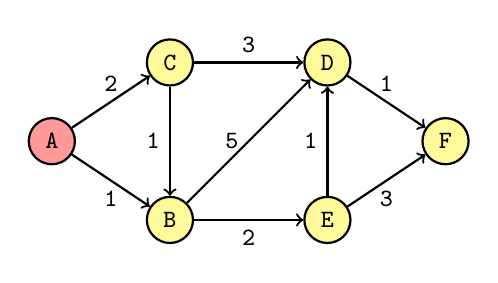
\begin{tikzpicture}[
	    thick,
	    font=\ttfamily\bfseries\small
	]
	\tikzset{
	    mynode/.style = {circle, draw=black, align=center,fill=yellow!40},
	    mynoder/.style = {circle, draw=black, align=center,fill=red!40},
	    edgen/.style = {->,thick},
	    edger/.style = {->,ultra thick,red}
	}
	\node[mynoder] at (0.0,1.0) (a) {A};
	\node[mynode]  at (1.5,0.0) (b) {B};
	\node[mynode]  at (1.5,2.0) (c) {C};
	\node[mynode]  at (3.5,2.0) (d) {D};
	\node[mynode]  at (3.5,0.0) (e) {E};
	\node[mynode]  at (5.0,1.0) (f) {F};
	\draw[edgen] (a) edge node[below] {1} (b);
	\draw[edgen] (a) edge node[above] {2} (c);
	\draw[edgen] (c) edge node[left] {1} (b);
	\draw[edgen] (c) edge node[above] {3} (d);
	\draw[edgen] (b) edge node[left] {5} (d);
	\draw[edgen] (b) edge node[below] {2} (e);
	\draw[edgen] (e) edge node[below] {3} (f);
	\draw[edgen] (e) edge node[left] {1} (d);
	\draw[edgen] (d) edge node[above] {1} (f);
	\end{tikzpicture}
\end{minipage}%
\begin{minipage}[c]{0.5\textwidth}\centering
	\begin{tabular}{@{} c ? *{7}{c} @{}}
		&&A&B&C&D&E&F \\
	\thickrule
		A & 0 & \textbf{0} & \(\cancel{0}\) & \(\cancel{0}\) & \(\cancel{0}\) & \(\cancel{0}\) & \(\cancel{0}\) \\
		B & \(\infty\) & 1 & \textbf{1} & \cancel{1} & \cancel{1} & \cancel{1} & \cancel{1} \\
		C & \(\infty\) & 2 & 2 & \textbf{2} & \cancel{2} & \cancel{2} & \cancel{2} \\
		D & \(\infty\) & \(\infty\) & 6 & 5 & 4 & \textbf{4} & 4\\
		E & \(\infty\) & \(\infty\) & 3 & 3 & \textbf{3} & \cancel{3} & \cancel{3} \\
		F & \(\infty\) & \(\infty\) & \(\infty\) & \(\infty\) & 6 & 5 & \textbf{5} \\
	\end{tabular}
\end{minipage}

\begin{itemize}
	\item ogni colonna contiene lo stato del vettore $d$ all'inizio di ogni ripetizione del ciclo \textsf{while} \Not S.\setEmpty
	\item ogni riga \(v\) rappresenta l'evoluzione dello stato dell'elemento \(d[v]\);
	\item la legenda delle colonne rappresenta il nodo che viene estratto.
\end{itemize}

\paragraph{Correttezza}
Tutte le volte che estraiamo un nodo, quel nodo ha una distanza (priorità) positiva ed estraiamo nodi a distanza progressivamente crescenti.
Se estraggo un nodo dalla coda tutti gli altri nodi hanno distanze più grandi.
Tutte le volte che estraggo un nodo la sua distanza non può più essere modificata.
Ed è questo il motivo per cui l'algoritmo di Dijkstra funziona (bene) solo con pesi positivi.

\begin{note}
L'algoritmo di Dijkstra funziona correttamente solo con pesi positivi.
\end{note}

\subsection{Correttezza per pesi positivi}

Ogni nodo viene estratto una e una sola volta.
Al momento dell'estrazione la sua distanza è minima.

\begin{proof}[Dimostrazione per induzione sul numero \(k\) di nodi estratti]
Per \(k=0\) (caso base) è vero poiché \mbox{\(d[s]=0\)} e non ci sono lunghezze negative.
Supponiamo che sia vero per i primi \(k-1\) nodi (ipotesi induttiva).
Quando viene estratto il \(k\)-esimo nodo \(u\), la sua distanza \(d[u]\) dipende dai \(k-1\) nodi già estratti (passo induttivo).
Non può quindi dipendere dai nodi ancora da estrarre, che hanno distanza \(\geqslant d[u]\).
Di conseguenza \(d[u]\) è minimo e \(u\) non verrà più re-inserito, perché non ci sono distanze negative.
\end{proof}

\section{Algoritmo di Johnson}

\paragraph{Analisi della complessità}
% \(\Omicron(n^2 + m)\) ma siccome \(m = \Omicron(n^2)\), allora il costo è \(\Omicron(n^2)\).
Con l'introduzione dell'heap binario nel '64 le operazioni che prima venivano svolte con complessità \(\Omicron(n)\) sul vettore ordinato ora hanno complessità \(\Omicron(\log n)\).
Di conseguenza la complessità totale dell'algoritmo scende da \(\Omicron(n^2)\) a \(\Omicron(m \log n)\).

Per \emph{grafi densi} non conviene utilizzare uno heap binario in quanto \(m = \Theta(n^2)\) e di conseguenza l'algoritmo avrebbe una complessità di \(\Omicron(n^2 \log n)\) si preferisce quindi la versione con vettore ordinato per una complessità di \(\Omicron(n^2)\), mentre per \emph{grafi sparsi} \(m = \Theta(n)\) e l'algoritmo \(\Omicron(n \log n)\) che è migliore di \(\Omicron(m \log n)\).

\section{Algoritmo di Fredman-Tarjan}

\paragraph{Analisi della complessità}
Sfruttando un heap di fibonacci l'operazione di \heapDecrease ha costo ammortizzato costante; così facendo hanno abbassato la complessità a \(\Omicron(m + n \log n)\).
Per \emph{grafi sparsi} produce un miglioramento nella complessità.

\section{Algoritmo di Bellman-Ford-Moore}

\begin{note}
\'E computazionalmente più pesante dell'algoritmo di Dijkstra ma può lavorare anche con archi di peso negativo.
\end{note}

\paragraph{Implementazione}
Utilizza una coda senza priorità.

\begin{algorithm}[H]
	\caption{Algoritmo di Bellman-Ford-Moore}
	%&../preamble

% \documentclass[varwidth=6in]{standalone}
% \usepackage{../preamble}

% arara: pdflatex: { synctex: no }
% arara: latexmk: { clean: partial }
\ifstandalone
\begin{document}
\NoCaptionOfAlgo
\begin{algorithm}[H]
\caption[Bellman-Ford-Moore]{}
\fi

\prototype{\Array{\Int}, \Array{\Int} \CamminiMinimi{\Graph \(G\), \Node \(s\)}}{

	\BlankLine
	\lnl{bellman:init}%
	\alert{ \Queue \(S\) \Assign \queueConstructor }\;
	\alert{ \(S.\queueInsert{s}\) } \Comment*[h]{metto in coda la sorgente}\;

	\BlankLine
	\While(\Comment*[h]{\(\Omicron(n)\)}){\Not \(S\).\setEmpty}{

		\lnl{bellman:remove}%
		\alert{ \Int \(u\) \Assign \(S\).\queueRemove } \Comment*[l]{\(\Omicron(1 \cdot n)\)}
		\ArrayCall{b}{u} \Assign \False\;

		\BlankLine
		\ForEach{\( v \in G.\adj{u} \)}{
			\If{\( \ArrayCall{d}{u} + G.\weight{u,v} < \ArrayCall{d}{v} \)}{

				\BlankLine
				\If{\Not \ArrayCall{b}{v}}{
					\lnl{bellman:add}%
					\tcp{lo metto in cosa quando c'è un miglioramento}
					\alert{ \(S.\queueInsert{v}\) } \Comment*[h]{\(\Omicron(m \cdot n)\)}\;
					\ArrayCall{b}{v} \Assign \True\;
				}

				\ArrayCall{T}{v} \Assign \(u\)\;
				\ArrayCall{d}{v} \Assign \(\ArrayCall{d}{u} + G.\weight{u,v}\)\;
			}
		}
	}
	\Return \((T, d)\)\;
}

\ifstandalone
\end{algorithm}
\RestoreCaptionOfAlgo
\end{document}
\fi

\end{algorithm}

\begin{itemize}
	\item [\circled{\ref{bellman:init}}]
	Viene creata una coda di dimensione \(n\).
	Per un costo computazionale di \(O(n)\);
	\item [\circled{\ref{bellman:remove}}]
	Viene estratto il prossimo elemento della coda.
	Per un costo computazionale di \(O(1)\);
	\item [\circled{\ref{bellman:add}}]
	Si inserisce l'indice \(v\) in coda.
	Per un costo computazionale di \(O(1)\).
\end{itemize}

L'inserimento in coda può essere fatto più di una volta durante il ciclo di esecuzione dell'algoritmo, al contrario di quel che accade nell'algoritmo di Dijkstra.
Il passo \circled{4} non è necessario in quanto non c'è una priorità da aggiornare.

\subsubsection*{Esempio di esecuzione}

\begin{minipage}[c]{0.5\textwidth}\centering
	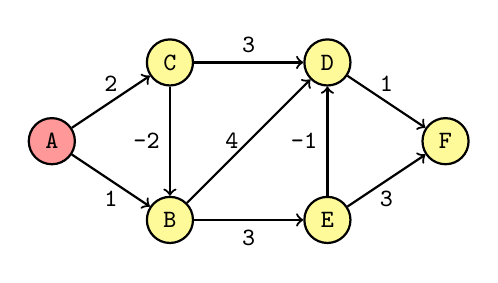
\begin{tikzpicture}[
	    thick,
	    font=\ttfamily\bfseries\small
	]
	\tikzset{
	    mynode/.style = {circle, draw=black, align=center,fill=yellow!40},
	    mynoder/.style = {circle, draw=black, align=center,fill=red!40},
	    edgen/.style = {->,thick},
	    edger/.style = {->,ultra thick,red}
	}
		\node[mynoder] at (0.0,1.0) (a) {A};
		\node[mynode]  at (1.5,0.0) (b) {B};
		\node[mynode]  at (1.5,2.0) (c) {C};
		\node[mynode]  at (3.5,2.0) (d) {D};
		\node[mynode]  at (3.5,0.0) (e) {E};
		\node[mynode]  at (5.0,1.0) (f) {F};
		\draw[edgen] (a) edge node[below] {1} (b);
		\draw[edgen] (a) edge node[above] {2} (c);
		\draw[edgen] (c) edge node[left] {-2} (b);
		\draw[edgen] (c) edge node[above] {3} (d);
		\draw[edgen] (b) edge node[left] {4} (d);
		\draw[edgen] (b) edge node[below] {3} (e);
		\draw[edgen] (e) edge node[below] {3} (f);
		\draw[edgen] (e) edge node[left] {-1} (d);
		\draw[edgen] (d) edge node[above] {1} (f);
	\end{tikzpicture}
\end{minipage}%
\begin{minipage}[c]{0.5\textwidth}
\paragraph{Come leggere la tabella sottostante}
\begin{itemize}[leftmargin=*]
	\item la prima riga contiene l'elemento estratto dalla coda;
	\item l'ultima riga contiene lo stato della coda;
	\item i vettori delle distanze sono rappresentate dalle colonne.
\end{itemize}
\end{minipage}

\begin{table}[H]\centering
	\begin{tabu}{ r @{\hskip 5pt} >{\ttfamily\small}c ? c | c  | cc | ccc | ccc | c | c @{\hskip 5pt}}
		\rowfont{\ttfamily\small}
			nodo estratto:& & & A & B & C & D & E & B & F & D & E & D & F \\
		\Xcline{2-14}{1pt}
			\multirow[c]{6}{*}{\rotatebox[origin=c]{90}{vettori}}
						   & A & 0 & 0 & 0 & 0 & 0 & 0 & 0 & 0 & 0 & 0 & 0 & 0 \\
						   & B & \(\infty\) & 1 & 1 & 0 & 0 & 0 & 0 & 0 & 0 & 0 & 0 & 0 \\
						   & C & \(\infty\) & 2 & 2 & 2 & 2 & 2 & 2 & 2 & 2 & 2 & 2 & 2 \\
						   & D & \(\infty\) & 5 & 5 & 5 & 3 & 3 & 3 & 3 & 3 & 2 & 2 & 2 \\
						   & E & \(\infty\) & \(\infty\) & 4 & 4 & 4 & 4 & 3 & 3 & 3 & 3 & 3 & 3 \\
						   & F & \(\infty\) & \(\infty\) & \(\infty\) & \(\infty\) & 6 & 5 & 5 & 5 & 4 & 4 & 3 & 3 \\
		\Xcline{2-14}{1pt}\rowfont{\ttfamily\small}
	 			queue:& S & A & BC & CDE & DEB & EBF & BFD & FDE & DE & E & D & F & \\
	\end{tabu}
\end{table}

\paragraph{Dimostrazione di correttezza}
Per dimostrare la correttezza dell'algoritmo dobbiamo dare la definizione di \enquote{passata}.
Una passata si definisce ricorsivamente come segue: per \(k = 0\), la zeresima passata consiste nell'estrazione del nodo \(s\) dalla coda \(S\), per \(k > 0\) la \(k\)-esima passata consiste nell'estrazione di tutti i nodi presenti in \(S\) al termine della passata \(k-1\)-esima.
Viene data solo un'intuizione, non viene fatta una dimostrazione formale.
Al termine della passata \(k\), i vettori \(T\) e \(d\) descrivono i cammini minimi di lunghezza al più \(k\).
Al termine della passata \(n-1\), i vettori \(T\) e \(d\) descrivono i cammini (di lunghezza al più \(n-1\)).

\paragraph{Analisi della complessità}
L'inserimento in coda dei nodi avviene solo una volta per un costo di \(\Omicron(1)\).
Un nodo può essere estratto e reinserito al massimo \(n-1\) volte, per un costo di \(\Omicron(n^2)\).
Quando avviene un miglioramento la distanza viene aggiornata, per un costo i \(\Omicron(n \dot m)\).
Il costo complessivo dell'algoritmo risulta quindi \(\Omicron(n \dot m)\).

\paragraph{Cammini minimi su DAG}
I cammini minimi su DAG sono sempre ben definiti;
anche in presenza di pesi negativi, in quanto non esistono cicli (nè tantomeno quelli negativi).
\'E possibile rilassare gli archi \emph{in ordine topologico}, \emph{una volta sola}.
Non essendoci cicli, non c'è modo di tornare su un nodo già visitato ed abbassare il valore della sua distanza (il suo campo \(d\)).

Si utilizza quindi l'ordine topologico.

\begin{algorithm}[H]
	\caption{Algoritmo di Bellman-Ford-Moore applicato su DAG}
	%&../preamble

% arara: pdflatex: { synctex: no }
% arara: latexmk: { clean: partial }
\ifstandalone
\begin{document}
\begin{algorithm}[H]
\fi

(\Array{\Int}, \Array{\Int})\prototype{\ \CamminiMinimi{\Graph \(G\), \Node \(s\)}}{

	\BlankLine
	\Array{\Int} \(d =\) \new \Array{\Int}[1][G.n] \Comment*[r]{\(d[u]\) è la distanza da \(s\) a \(u\)}
	\Array{\Int} \(T =\) \new \Array{\Int}[1][G.n] \Comment*[r]{\(T[u]\) è il padre da \(u\) nell'albero \(T\)}

	\BlankLine
	\tcp{Inizializzo i vettori}
	\ForEach{\(u \in G.\VV - \{s\}\)}{
		\(T[u] = \Nil\)\;
		\(d[u] = +\infty\)\;
	}

	\BlankLine
	\tcp{Inizializzo la sorgente}
	\(T[s] = \Nil\)\;
	\(d[u] = 0\)\;

	\BlankLine
	\tcp{Effettuo l'ordinamento topologico dei nodi nel DAG}
	\Stack \(S = \topSort\)\;

	\BlankLine
	\tcp{fintanto che la pila non è vuota}
	\While{\Not \(S.\setEmpty\)}{
		\(u = S.\stackPop\) \tcp{estraggo un nodo}
		\ForEach(\tcp*[h]{per ogni nodo adiacente}){\(v \in G.\adj{v}\)}{
			\If(\tcp*[h]{se il peso è migliore di quello presente}){\(d[u] + G.\weight{u,v} < d[v]\)}{

				\BlankLine
				\tcp{aggiorno il peso}
				\(T[v] = u\)\;
				\(d[v] = d[u] + G.\weight{u,v}\)\;
			}
		}
	}

	\BlankLine
	\tcp{restituisco il vettore dei padri e il vettore delle distanze}
	\Return (\(T\), \(d\))\;
}

\ifstandalone
\end{algorithm}
\end{document}
\fi

\end{algorithm}

\subsection{Riassumendo}

\begin{table}[H]\centering
	\caption{Quale complessità preferire?}%
	\label{tab:complexity-compared}
	\begin{tabular}{@{} *{4}{l} @{}}\toprule
			\textbf{Algoritmo} & \textbf{Complessità} & \textbf{Input}\\
		\midrule
			Dijkstra		& \(\Omicron(n^2)\)				& Pesi positivi, grafi denso  \\
		\lightrule
			Johnson			& \(\Omicron(m \log n)\)		& Pesi positivi, grafi sparso \\
		\lightrule
			Fredman-Tarjan	& \(\Omicron(m + n \log n)\)	& Pesi positivi, grafi denso, dimensioni molto grandi \\
		\lightrule
			Bellman-Ford	& \(\Omicron(m \cdot n)\)		& Pesi negativi \\
							& \(\Omicron(m + n)\)			& DAG			\\
						\lightrule
			BFS				& \(\Omicron(m + n)\)			& Senza pesi	\\
		\bottomrule
	\end{tabular}
\end{table}

\subsection{Cammini minimi, sorgente multipla}

Vogliamo cercare i cammini minimi fra tutti i nodi.

\begin{table}[H]\centering
	\caption{Quale complessità preferire?}%
	\label{tab:complexity-compared}
	\begin{tabular}{@{} *{3}{l} @{}}
		\toprule
			\textbf{Algoritmo} & \textbf{Complessità} & \textbf{Input}\\
		\midrule
			Pesi positivi, grafo denso & \(\Omicron(n \cdot n^2)\) & Applicazione ripetuta (\(n\)) dell'algoritmo di Dijkstra \\
		\lightrule
			Pesi positivi, grafo sparso & \(O(n \cdot (m \log n))\) & Applicazione ripetuta dell'algoritmo di Johnson \\
		\lightrule
			Pesi negativi & \(O(n \cdot nm)\) & Applicazione ripetuta di Bellman-Ford (sconsigliata) \\
		\lightrule
			Pesi negativi, grafo denso & \(O(n^3)\) & Algoritmo di \textbf{Floyd e Warshall} \\
		\lightrule
			Pesi negativi, grafo sparso & \(O(nm \log n)\) & Algoritmo di \textbf{Johnson per sorgente multipla}\\
		\bottomrule
	\end{tabular}
\end{table}

L'algoritmo di Bellman-Ford è sconsigliato per grafi densi perché può arrivare ad avere una complessità di \(\Omicron(n^4)\), mentre l'algoritmo di Floyd e Warshall ha una complessità di \(\Omicron(n^3)\) indipendentemente dalla forma del grafo.

\section{Algoritmo di Floyd-Warshall}

Utilizza la programmazione dinamica.
Ci riesce ridefinendo la definione del costo di cammino in modo tale che possa essere calcolato in modo ricorsivo.

\begin{definition}[Cammini minimi \(k\)-vincolati]
Sia \(k\) un valore in \(\{0, \dots, n\}\).
Diciamo che un cammino \(p_{xy}^{k}\) è un cammino minimo \(k\)-vincolato fra \(x\) ed \(y\) se esso ha il costo minimo fra tutti i cammini fra \(x\) e \(y\) che non passano per nessun vertice in \(v_{k+1}, \dots, v_n\) (\(x\) e \(y\) sono esclusi dal vincolo).
\end{definition}

\begin{note}
Assumiamo, come abbiamo sempre fatto, che esista un ordinamento fra i nodi del grafo \(v_1, v_2, \dots, v_n\).
\end{note}

% \(p_{xy}^{0}\) corrisponde a
% \(p_{xy}^{n}\) corrisponde a

\begin{definition}[Distanza \(k\)-vincolata]
Denotiamo con \(d^{k}[x][y]\) il costo totale del cammino minimo \(k\)-vincolato fra \(x\) e \(y\), se esiste.
\[
d^{k}[x][y] =
	\begin{dcases}
		w(p_{xy}^{k}) & \text{se esiste }p_{xy}^{k}\\
		+\infty & \text{altrimenti}\\
	\end{dcases}
\]
\end{definition}

% \(d^{0}[x][y]\) corrisponde a
% \(d^{n}[x][y]\) corrisponde a

La formulazione ricorsiva è la seguente:
\[
d^{k}[x][y] =
	\begin{dcases}
		d[x][y] & k = 0\\
		d^{k-1}[x][y] \lor d^{k-1}[x][k] \land d^{k-1}[k][y] & k > 0\\
	\end{dcases}
\]
Ad esempio:

% TODO esternare le immagini
\begin{minipage}[c]{0.5\textwidth}\centering
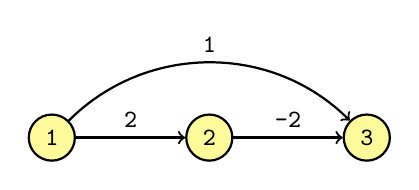
\begin{tikzpicture}[
    thick,
    font=\ttfamily\bfseries\small
]
	\tikzset{
	    mynode/.style = {circle, draw=black, align=center,fill=yellow!40},
	    mynoder/.style = {circle, draw=black, align=center,fill=red!40},
	    edgen/.style = {->,thick},
	    edger/.style = {->,ultra thick,red}
	}
	\node[mynode] at (0.0,0.0) (a) {1};
	\node[mynode] at (2.0,0.0) (b) {2};
	\node[mynode] at (4.0,0.0) (c) {3};
	\draw[edgen] (a) edge node[above] {2} (b);
	\draw[edgen] (b) edge node[above] {-2} (c);
	\draw[edgen] (a) edge[bend left=45] node[above] {1} (c);
\end{tikzpicture}
\end{minipage}%
\begin{minipage}[c]{0.5\textwidth}\centering
\begin{align*}
d^{0}[1][3] &= 1 \\
d^{1}[1][3] &= 1 \\
d^{2}[1][3] &= \minFunction(d^{1}[1][3], d^{1}[1][2] + d^{2}[2][3]) \\
			&= \minFunction(1, +2-2) \\
			&= \minFunction(1, 0) = 0 \\
\end{align*}
\end{minipage}

% TODO [39-40]

Oltre a definire la matrice \(d\), calcoliamo una matrice \(T\) dove \(T[x][y]\) rappresenta il predecessore di \(y\) nel cammino più breve da \(x\) a \(y\).
Ad esempio:

\begin{minipage}[c]{0.5\textwidth}\centering
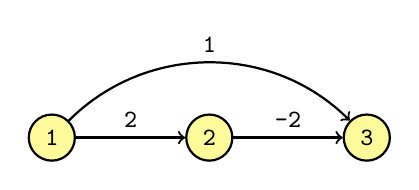
\begin{tikzpicture}[
    thick,
    font=\ttfamily\bfseries\small
]
	\tikzset{
	    mynode/.style = {circle, draw=black, align=center,fill=yellow!40},
	    mynoder/.style = {circle, draw=black, align=center,fill=red!40},
	    edgen/.style = {->,thick},
	    edger/.style = {->,ultra thick,red}
	}
	\node[mynode] at (0.0,0.0) (a) {1};
	\node[mynode] at (2.0,0.0) (b) {2};
	\node[mynode] at (4.0,0.0) (c) {3};
	\draw[edgen] (a) edge node[above] {2} (b);
	\draw[edgen] (b) edge node[above] {-2} (c);
	\draw[edgen] (a) edge[bend left=45] node[above] {1} (c);
\end{tikzpicture}
\end{minipage}%
\begin{minipage}[c]{0.5\textwidth}\centering
\begin{align*}
T[1][2] &= 1 \\
T[2][3] &= 2 \\
T[1][3] &= 2 \\
\end{align*}
\end{minipage}

% TODO scrivere l'algoritmo
\begin{algorithm}[H]
	\caption{Algoritmo di Floyd-Warshall}
	%&../preamble

% arara: pdflatex: { synctex: no }
% arara: latexmk: { clean: partial }
\ifstandalone
\begin{document}
\begin{algorithm}[H]
\fi

(\Array{\Int}, \Array{\Int})\prototype{\ \CamminiMinimi{\Graph \(G\), \Node \(s\)}}{

	\BlankLine
	\tcp{Credo le matrici}
	\Matrix{\Int} \(d =\) \new \Matrix{\Int}[1\dots n][1\dots n] \Comment*[r]{matriche delle distanze}
	\Matrix{\Int} \(T =\) \new \Matrix{\Int}[1\dots n][1\dots n] \Comment*[r]{matriche dei padri (predecessori)}

	\BlankLine
	\tcp{Inizializzo i vettori}
	\ForEach{\(u, v \in G.\VV\)}{
		\(d[u][v] = +\infty\)\;
		\(T[u][v] = \Nil\)\;
	}

	\BlankLine
	\tcp{Inserisco i valori iniziali}
	\ForEach{\(u \in G.\VV\)}{
		\ForEach{\(v \in G.\adj{u}\)}{
			\(d[u][v] = G.\weight(u, v)\)\;
			\(T[u][v] = u\)\;
		}
	}

	\BlankLine
	\tcp{Aggiorno le distanze}
	\From{\(k \Assign 1\) \DownTo \(G.n\)}{
		\ForEach{\(u \in G.\VV\)}{
			\ForEach{\(v \in G.\adj{u}\)}{
				\If{\( d[u][k] + d[k][v] < d[u][v] \)}{
					\(d[u][v] = d[u][k] + d[k][v]\)\;
					\(T[u][v] =T[k][v]\)\;
				}
			}
		}
	}

	\BlankLine
	\Return \(d\)\;
}

\ifstandalone
\end{algorithm}
\end{document}
\fi

\end{algorithm}

\section{Algoritmo di Warshall}

\begin{definition}[Chiusura transitiva]
La chiusura transitiva \(G^* = (V, E^*)\) di un grafo \(G = (V, E)\) è il grafo orientato tale che \((u, v) \in E^*\) se e solo esiste un cammino da \(u\) a \(v\) in \(G\).
\end{definition}

Supponendo di avere il grafo \(G\) rappresentato da una matrice di adiacenza \(M\), la matrice \(M^n\) rappresenta la matrice di adiacenza di \(G^*\).

La formulazione ricorsiva è la seguente:
\[
M^{k}[x][y] =
	\begin{dcases}
		M[x][y] & k = 0\\
		M^{k-1}[x][y] \lor M^{k-1}[x][k] \land M^{k-1}[k][y] & k > 0\\
	\end{dcases}
\]

\section*{Conclusioni}

Abbiamo visto una panoramica dei più importanti algoritmi per la ricerca dei cammini minimi.
Esistono anche altri algoritmi, in particolare l'algortimo \(A^*\) utilizza euristiche per velocizzare la ricerca.

\end{document}

	% %&../settings/preamble.main

\ifsubfile
% ATTENTION non modificare "development", viene modificata automaticamente in deploy
\newcommand{\docversion}{development}
\usepackage{../settings/subfile}
\setcounter{chapter}{12}

\usepackage[newfloat, cachedir=_minted-cache, outputdir=../build]{minted}
\usepackage{../libraries/set-minted}

% \usepackage{debug}

% arara: pdflatex: { options: ["--output-directory=../build"], shell: yes, draft: yes, synctex: no }
% arara: pdflatex: { options: ["--output-directory=../build"], shell: yes, synctex: no }
\begin{document}
\fi
\tagThisPage
\chapter{Programmazione Dinamica}
\epigraph{\enquote{Those who cannot remember the past are condemned to repeat it.}}%
         {--- \textup{\textsc{George Santayana}, \emph{The Life of Reason} (1905)}}

\section*{Introduzione}

La programmazione dinamica è un metodo per spezzare ricorsivamente un problema in
sottoproblemi, i quali vengono risolti una volta sola e la loro soluzione viene memorizzata in una tabella.
Nel caso il sottoproblema debba essere risolto nuovamente, si recupera la soluzione dalla tabella.
La tabella è facilmente indirizzabile: la sua consultazione (\lookup) costa \(\Omicron(1)\).

\begin{figure}[!ht]
    \centering
    \includegraphics[width=.65\textwidth]{progrdyn}
    \caption{Approccio generale ad un problema per capire quale tecnica utilizzare}
\end{figure}

Le soluzioni dei sottoproblemi confluiscono nella tabella delle soluzioni, nel caso stia risolvendo un problema di conteggio allora posso restituire immediatamente la soluzione, altrimenti ho un meccanismo (la tabella) per ricostruire la soluzione ottima.

\subsection*{La programmazione dinamica nella storia}

Il termine \foreign{Dynamic Programming} è stato coniato da Richard Bellman agli inizi degli anni '50, nell'ambito dell'ottimizzazione matematica.
Inizialmente, si riferiva al processo di risolvere un problema compiendo le migliori decisioni una dopo l'altra.
\enquote{\foreign{Dynamic}} doveva dare un senso \enquote{temporale}, mentre \enquote{\foreign{Programming}} si riferiva all'idea di creare \enquote{programmazioni ottime}, per esempio nella logistica.
\`{E} possibile approfondire all'indirizzo \url{https://en.wikipedia.org/wiki/Dynamic_programming#History}.

La \emph{programmazione dinamica} è caratterizzata da 4 fasi principali:
\begin{enumerate}
    \item caratterizzare \emph{matematicamente} la struttura di una soluzione ottima;
    \item definire ricorsivamente il valore di una soluzione ottima;
    \item calcolare il valore di una soluzione ottima con approccio \foreign{bottom-up} ed utilizzare una tabella per memorizzare la soluzione dei sottoproblemi  ed utilizzarla per evitare di ripetere i calcoli più volte;
    \item ricostruire la soluzione ottima.
\end{enumerate}

\clearpage
\section{Domino lineare}

\paragraph{Definizione del problema}
Il gioco del domino è basato su tessere di dimensione \(2 \times 1\).
Scrivere un algoritmo efficiente che prenda in input un intero \(n\) e restituisca il numero di possibili disposizioni di \(n\) tessere in un rettangolo \(2 \times n\).

\begin{figure}[H]\centering
    \includegraphics[width=1\textwidth]{domino}
    \caption[]{Rappresentazione delle cinque disposizioni possibili con cui è possibile riempire un rettangolo \(2 \times 4\).}
\end{figure}

\subsubsection{Definizione ricorsiva}

Definiamo una formula ricorsiva \(DP[n]\) che ci permetta di calcolare il numero di disposizioni possibili quando si hanno \(n\) tessere.
Con nessuna tessera (\(n=0\)) esiste una sola disposizione possibile.
Avendo a disposizione una tessera (\(n=1\)) è possibile disporla solo verticalmente.

Se posiziono una tessera in verticale, risolverò il problema di dimensione \(n-1\), mentre se la posiziono in orizzontale ne devo mettere due, risolvendo così il problema di dimensione \(n-2\).
Queste ultime due possibilità si sommano insieme (conteggio).
\[
    DP(n) =
    \begin{dcases}
    1                 & n \leqslant 1 \\
    DP[n-2] + DP[n-1] & n > 1 \\
    \end{dcases}
\]

La serie generata è una successione di Fibonacci.
\(DP[n]\) infatti è pari al \(n + 1\)-esimo numero della serie.

\subsubsection{Algoritmo ricorsivo}

L'algoritmo che viene scaturito dalla definizione ricorsiva del problema è il seguente:

\begin{algorithm}[H]
    \caption{Algoritmo \emph{ricorsivo} che risolve il problema Domino}
    %&../preamble

% arara: pdflatex: { synctex: no }
% arara: latexmk: { clean: partial }
\ifstandalone
\begin{document}
\begin{algorithm}[H]
\fi

\prototype{\Int \fibonacciRic{\Int n}}{
	\eIf{\( n \leqslant 1 \)}{
		\Return \(1\)\;
	}{
		% \tcp{due chiamate ricorsive \(time \to \Omicron(2^n)\)}
		\Return \(\fibonacciRic{\(n-1\)} + \fibonacciRic{\(n-2\)}\)\;
	}
}

\ifstandalone
\end{algorithm}
\end{document}
\fi

\end{algorithm}

\paragraph{Analisi della complessità}
L'equazione di ricorrenza associata a \fibonacciRic è la seguente:
\[
    T(n) =
    \begin{dcases}
    1                   & n \leqslant 1 \\
    T(n-1) + T(n-2) + 1 & n > 1 \\
    \end{dcases}
\]
\`{E} una ricorrenza lineare di ordine costante, per calcolare la sua complessità applichiamo quindi il \foreign{master theorem}: i fattori moltiplicativi di \(T(n-1)\) e \(T(n-2)\) sono \(a_1 = 1\) e \(a_2 = 1\) rispettivamente, possiamo raccogliergli in \(a = a_1 + a_2 = 2\), il fattore \(\beta\) risulta pari a \(0\), in quanto \(n^0=1\).
Possiamo concludere che la complessità dell'algoritmo è \(\Theta(a^n \cdot n^\beta) = \Theta(2^n)\).

L'albero di ricorsione generato dall'algoritmo è quello mostrato in~\cref{fig:fibonacci-tree}.

\begin{figure}[H]\centering
    \includegraphics[width=.7\textwidth]{fibonacci-tree}
    \caption[Albero di ricorsione in cui si possono notare problemi ripetuti]
            {Albero di ricorsione per \fibonacciRic. Possiamo notare che molti sottoproblemi vengono ripetuti.}%
    \label{fig:fibonacci-tree}
\end{figure}

\subsubsection{Come evitare di risolvere un problema più di una volta}

Dalla~\cref{fig:fibonacci-tree} possiamo notare che molti sottoproblemi vengono ripetuti.
Per evitare che questo avvenga memorizziamo il risultato ottenuto risolvendo un particolare
problema in una \textbf{tabella DP}, la quale sarà un vettore, una matrice o un dizionario dipendentemente dalle nostre esigenze.
La tabella conterrà un elemento per ogni sottoproblema che dobbiamo risolvere.
Memorizzeremo i casi base nelle relative posizioni.
Dopodiché l'iterazione sarà \foreign{bottom-up}: partiremo dai casi base e andremo verso problemi via via sempre più grandi fino a risolvere il problema originale.

\begin{algorithm}[H]
    \caption[Algoritmo iterativo per Domino]
            {Algoritmo \emph{iterativo} per Domino}
    \documentclass[varwidth=6in]{standalone}
\usepackage{../_preamble}

% arara: pdflatex: { synctex: no }
% arara: latexmk: { clean: partial }
\begin{document}
\ifstandalone
\NoCaptionOfAlgo
\begin{algorithm}[H]
\caption[Fibonacci iterativo]{}
\fi

\prototype{\Int \fibonacciIter{\Int \(n\)}}{

	\BlankLine
	\(DP\) \Assign \new \Array{\Int}{0}{n}\;
	\ArrayCall{DP}{0} \Assign \ArrayCall{DP}{1} \Assign 1\;

	\BlankLine
	\From{\(i \Assign 2\) \DownTo \(n\)}{
		\ArrayCall{DP}{i} \Assign \(\ArrayCall{DP}{i-1} + \ArrayCall{DP}{i-2}\)\;
	}

	\BlankLine
	\Return \ArrayCall{DP}{n}\;
}

\ifstandalone
\end{algorithm}
\RestoreCaptionOfAlgo
\fi
\end{document}

\end{algorithm}

\begin{table}[H]\centering
    \caption[]
            {I casi base vengono inseriti manualmente nelle relative posizioni.\\
             Ogni valore \(i\)-esimo successivo viene computato sulla base dei suoi valori precedenti \(i-1\) e \(1-2\)}
    \includegraphics[width=.4\textwidth]{fib-table1}
\end{table}

\paragraph{Analisi della complessità}
% La complessità in tempo è lineare, come lo è la complessità spaziale.
La complessità in tempo è \(T(n) = \Theta(n)\), quella in spazio è \(S(n) = \Theta(n)\).
\`{E} possibile migliorare l'algoritmo riducendo lo spazio utilizzato.

\subsubsection{Ottimizzazione dello spazio utilizzato}

\begin{algorithm}[H]
    \caption[Algoritmo iterativo che ottimizza lo spazio utilizzato per Domino]
            {Algoritmo \emph{iterativo che ottimizza lo spazio utilizzato} per Domino}
    %&../preamble

% arara: pdflatex: { synctex: no }
% arara: latexmk: { clean: partial }
\ifstandalone
\begin{document}
\begin{algorithm}[H]
\fi

\prototype{\Int \fibonacci{\Int n}}{
	\Int \(DP_0 \Assign 1\)\;
	\Int \(DP_1 \Assign 1\)\;
	\Int \(DP_2 \Assign 1\)\;

	\BlankLine
	\From{\(i \Assign 2\) \DownTo \(n\)}{
		\(DP_0 \Assign DP_1\)\;
		\(DP_1 \Assign DP_2\)\;
		\(DP_2 \Assign DP_0 + DP_1\)\;
	}

	\Return \(DP_2\)\;
}

\ifstandalone
\end{algorithm}
\end{document}
\fi

\end{algorithm}
\paragraph{Analisi della complessità}
Questa implementazione ha costo costante nello spazio \(S(n) = \Theta(1)\).

\renewcommand\arraystretch{1.4}
\begin{table}[H]\centering
    % \includegraphics[width=.4\textwidth]{fib-table2}
    \begin{tabular}{@{} C ? *{7}{C|} C @{}}
        n & 0 & 1 & 2 & 3 & 4 & 5 & 6 & 7 \\
    \thickrule
        {DP[n]_0} & - & - & 1 & 1 & 2 & 3 & 5 & 8 \\
        {DP[n]_1} & \emph{1} & \emph{1} & 1 & 2 & 3 & 5 & 8 & 13 \\
        {DP[n]_2} & \emph{1} & \emph{1} & 2 & 3 & 5 & 8 & 13 & 21 \\
    \end{tabular}
\end{table}
\renewcommand\arraystretch{1}

Sotto il modello di costo logaritmico (vedi~\cref{sec:valutare-dimensione-input}), le tre versioni hanno le complessità mostrate nella~\cref{tab:fibonacci-versions}.

\begin{table}[H]\centering
    \caption{Confronto delle varie versioni della funzione di fibonacci}\label{tab:fibonacci-versions}
    \begin{tabular}{@{} ll cc @{}}
    \toprule
        Funzione & Tipologia & \(T(n)\) & \(S(n)\) \\
    \midrule
        \fibonacciRic &  ricorsiva & \(\Omicron(n2^n)\) & \(\Omicron(n^2)\) \\
    \lightrule
        \fibonacciIter &  iterativa & \(\Omicron(n^2)\) & \(\Omicron(n^2)\) \\
    \lightrule
        \fibonacci &  finale & \(\Omicron(n^2)\) & \(\Omicron(n)\) \\
    \bottomrule
    \end{tabular}
\end{table}

Si può fare meglio di così utilizzando l'esponenziazione di matrici basata su quadrati (per approfondimenti consultare \url{https://brilliant.org/wiki/fast-fibonacci-transform/}).

\clearpage
\section{Hateville}

\paragraph{Descrizione del problema}
Hateville è un villaggio particolare, composto da \(n\) case, numerate da \(1\) a \(n\) lungo una singola strada.
Ad Hateville ognuno odia i propri vicini della porta accanto, da entrambi i lati.
Quindi il vicino \(i\) odia i vicini \(i-1\) e \(i+1\) (se esistenti).
Hateville vuole organizzare una sagra e vi ha affidato il compito di raccogliere i fondi.
Ogni abitante \(i\) ha intenzione di donare una quantità \(D[i]\), ma non intende partecipare ad una raccolta fondi a cui partecipano uno o entrambi i propri vicini.

Dobbiamo scrivere un algoritmo che restituisca la quantità massima di fondi che può essere raccolta.

\paragraph{Consegne del problema}
I problemi che possono esserci posti sono due:
\begin{enumerate}
    \item scrivere un algoritmo che restituisca la quantità massima di fondi che può essere raccolta;
    \item scrivere un algoritmo che restituisca il sottoinsieme di indici \(S \subseteq \{1, \dots, n\}\) tale per cui la donazione totale \(T = \sum_{i \in S} D[i]\) è massimale.
\end{enumerate}
se risolviamo il primo siamo ad un passo dalla soluzione del secondo, mentre se risolviamo il primo abbiamo risolto necessariamente il primo.

\paragraph{Esempi di esecuzione}
Con un vettore di donazioni \(D = [4, 3, 6]\) la raccolta massima è \(10\), dato dall'insieme di indici \(\{1, 3\}\).
Mentre con un vettore di donazioni \(D = [10, 5, 5, 10]\) la raccolta massima è \(20\), dato dall'insieme di indici \(\{1, 4\}\).

La domanda che dobbiamo porci è la seguente: è possibile ridefinire una formula ricorsiva che ci permetta di calcolare il sottoinsieme di case che, se selezionate, dà origine alla maggior quantità di donazioni?

\subsection{Definizione ricorsiva}

Ridefiniamo il problema caratterizzandolo matematicamente.

Definiamo \(HV(i)\) uno dei possibili insiemi di indici da selezionare per ottenere una donazione ottimale delle prime \(i\) case di Hateville, numerate \(1, \dots, n\).
\(HV(n)\) diventa quindi la soluzione del problema originale.

\subsubsection{Passo ricorsivo}

Andiamo per passi.
Consideriamo il vicino \(i\)-esimo.
\begin{itemize}
    \item cosa succede se \textbf{non accetto} la sua donazione?
    Lo scarto.
    Proviamo ad esprimerlo in funzione dei problemi precedenti (dopotutto il problema viene risolto in maniera ricorsiva):
    \[HV(i) = HV(i-1)\]

    \item cosa succede se \textbf{accetto} la sua donazione?
    Accetto la donazione \(i\)-esima e scarto i vicini.
    In simboli:
    \[HV(i) = \{i\} \cup HV(i-2)\]

    \item a questo punto come faccio a \textbf{decidere} quale delle due opzioni scegliere?
    Semplicemente prendo quello che mi dà un guadagno maggiore.
    In simboli:
    \[HV(i) = highest(HV(i-1), \{i\} \cup HV(i-2))\]
\end{itemize}
La funzione \(highest\) restituisce l'insieme di valore massimo.

\subsection*{Sottostruttura ottima}

Quando voglio provare che una soluzione di programmazione dinamica è corretta devo riuscire a dimostrare che le mie possibili scelte sono quelle giuste.
Per dimostrarlo utilizziamo il teorema di sottostruttura ottima, che dice sostanzialmente che il modo in cui ho applicato la ricorsione è corretto.

Proviamo quindi a dimostrare le scelte fatte.
Il problema dato dalle prime \(i\) case è indicato con \(HV_{p}(i)\) e una (ce ne può essere più di una) soluzione ottima per questo problema è indicato con \(HV_{s}(i)\).

Se \(i \not\in HV_{s}(i)\) allora \(HV_{s}(i) = HV_{s}(i-1)\) (ossia se l'\(i\)-esimo elemento non appartiene alla soluzione del problema \(HV_{s}i\) allora abbiamo scartare quella donazione \(HV_{s}(i-1)\)), altrimenti se l'abbiamo accettata e quindi \(i \in HV_{s}i\) allora \(HV_{s}(i) = HV_{s}(i-2) \cup \{i\}\).

Se abbiamo la soluzione ottima, allora possiamo dimostrare che abbiamo la soluzione ottima per i rispettivi sottoproblemi (da qui sottostruttura).

\begin{note}
Nella maggior parte dei casi non è necessaria una dimostrazione della soluzione, ma basta un'intuizione.
\end{note}

\subsection{Dimostrazione sottostruttura ottima}

Ricordiamo che indichiamo con \(HV_{p}(i)\) il problema dato dalle prime \(i\) case e con \(HV_{s}(i)\) una delle possibili soluzioni ottime per questo problema.
Indichiamo inoltre con \(\abs{HV_{s}(i)}\) l'ammontare di donazioni per la soluzione ottima \(HV_{s}(i)\).

\begin{note}
Dobbiamo dimostrare separatamente il caso in cui prendiamo la donazione \(i\)-esima e il caso in cui non la prendiamo, in quanto sono eventi mutualmente esclusivi.
\end{note}

Entrambe le dimostrazioni procedono per assurdo.

\begin{proof}[Dimostrazione caso 1: \(i {\protect\not\in} HV_{s}(i)\)]
Se non abbiamo preso la donazione \(i\)-esima vogliamo dimostrare che la soluzione ottima \(HV_{s}(i)\) è una soluzione ottima anche per il problema precedente \(HV_{p}(i-1)\).

Se così non fosse esisterebbe una soluzione (migliore) \(HV_{s}^{'} (i-1)\) per il problema \(HV_{p}(i-1)\) tale che l'ammontare delle donazioni del problema precedente sarebbe maggiore (in simboli \(\abs{HV_{s}^{'} (i-1)} > \abs{HV_{s}(i)}\)).
Ma allora \(HV_{s}^{'} (i-1)\) sarebbe una soluzione per \(HV_{p}(i)\)% (tale che \(\abs{HV_{s}^{'} (i-1)} > \abs{HV_{s}(i)}\))
, che è assurdo.
Quindi \(HV_{s}(i)\) è una soluzione ottima anche per \(HV_{p}(i-1)\).
\end{proof}

\begin{proof}[Dimostrazione caso 2: \(i \in HV_{s}(i)\)]
Se abbiamo preso l'\(i\)-esima donazione vogliamo dimostrare che \(i-1\) non appartiene alla soluzione ottima (in simboli \(i-1 \not\in HV_{s}(i)\)), altrimenti non sarebbe una soluzione ammissibile.
Quindi, se dalla soluzione ottima \(HV_{s}(i)\) togliessimo la donazione \(i\)-esima (\(HV_{s}(i) - \{i\}\)) questa dovrebbe essere una soluzione ottima per \(HV_{p} (i-2)\).

Se così non fosse, esisterebbe una soluzione \(HV_{s}^{'} (i-2)\) per il problema \(HV_{p} (i-2)\) tale che il suo guadagno sarebbe maggiore (in simboli \(\abs{HV_{s}^{'} (i-2)} > \abs{HV_{s} (i) - \{i\}}\)).
Ma allora \(HV_{s}^{'} (i-2) \cup \{i\}\) sarebbe una soluzione per \(HV_{p}(i)\)% (tale che \(\abs{HV_{s}^{'} (i-2) \cup \{i\}} > \abs{HV_{s} (i)}\))
, che è assurdo.
Quindi \(i-1 \not\in HV_s(i)\).
\end{proof}

\subsection{Completare la ricorsione}

Ragioniamo sui casi base.
Se ho \(0\) case il mio guadagno è zero: \(HV(0) = \emptyset\);
se ho una casa prendo semplicemente la sua donazione: \(HV(1) = \{1\}\).

Possiamo quindi scrivere la formula per calcolare la somma massima date \(i\) case:
\[
    HV(i) =
    \begin{dcases}
        0                                    & i = 0         \\
        \{1\}                                & i = 1         \\
        highest(HV(i-1), HV(i-2) \cup \{i\}) & i \geqslant 2 \\
    \end{dcases}
\]

Non vale la pena scrivere un algoritmo ricorsivo, basato su divide-et-impera, per risolvere il problema di Hateville poiché si risolverebbero molti sottoproblemi più volte.

\subsection{Memorizzare una tabella}

Facciamo qualche esempio di esecuzione.
Nel primo il vettore delle donazioni è \(D = [10, 5, 5, 8, 4, 7, 12]\), mentre nel secondo è \(D = [10, 1, 1, 10, 1, 1, 10]\).
Convincersi che gli insiemi risultanti sono corretti.

\begin{table}[H]\centering
    \begin{tabular}{@{} C *{8}{C} @{}}
    \toprule
        i & 0 & 1 & 2 & 3 & 4 & 5 & 6 & 7\\
    \midrule
        D & & 10 & 5 & 5 & 8 & 4 & 7 & 12\\
    \lightrule
        HV & \emptyset & \{1\} & \{1\} & \{1,3\} & \{1,4\} & \{1,3,5\} & \{1,4,6\} & \{1,3,5,7\}\\
    \bottomrule
    \end{tabular}
\end{table}

\begin{table}[H]\centering
    \begin{tabular}{@{} C *{8}{C} @{}}
    \toprule
        i & 0 & 1 & 2 & 3 & 4 & 5 & 6 & 7\\
    \midrule
        D &  & 10 & 1 & 1 & 10 & 1 & 1 & 10\\
    \lightrule
        HV & \emptyset & \{1\} & \{1\} & \{1,3\} & \{1,4\} & \{1,4\} & \{1,4,6\} & \{1,4,7\}\\
    \bottomrule
    \end{tabular}
\end{table}

A questo punto dobbiamo risolvere ancora due problemi:
\begin{enumerate}
    \item dobbiamo definire la funzione \(highest\) (ma è banale);
    \item dobbiamo memorizzare gli insiemi nella tabella.
\end{enumerate}
Memorizzare gli insiemi delle scelte nella tabella è costoso, quindi lo non faremo.
Costruiremo invece il valore della soluzione.
Così facendo eviteremo di memorizzare gli insiemi nella tabella e potremmo comunque ricostruire la soluzione a posteriori.

\subsubsection{Tabella di programmazione dinamica}

Indichiamo con \(DP[i]\) il \textbf{valore} della  massima quantità di donazioni che possiamo ottenere dalle prime \(i\) case di Hateville, e con \(DP[n]\) il valore della soluzione ottima.
%
Possiamo quindi riempire la tabella di programmazione dinamica nel seguente modo:
\[
    DP[i] =
    \begin{dcases}
        0                                  & i = 0 \\
        D[1]                               & i = 1 \\
    \maxFunction(DP[i-1], DP[i-2] + DP[i]) & i \geqslant 2 \\
    \end{dcases}
\]

Nel caso avessi \(0\) donatori allora la somma delle donazioni sarà \(0\).
Mentre nel caso abbia un solo donatore (\(i=1\)) allora prenderò la sua donazione (\(D[1]\)).
Infine nel caso avessi \(2\) o più donatori allora prendere una scelta: o scarterò quella donazione, quindi non considererò più quell'indice (\(DP[i-1]\)), o la accetter (\(+ DP[i]\)) e dovrò scartare a priori la scelta del suo vicino (\(DP[i-2]\)).
La sceltà è rappresentata dalla funzione \maxFunction che selezionerà quale fra le due scelte sarà quella più conveniente.

\begin{note}
Non memorizziamo più insiemi, ma valori.
Infatti non effettuiamo più l'unione di insiemi ma la somma fra i valori contenuti all'interno della tabella.
\end{note}

Dall'equazione di ricorrenza possiamo scrivere in modo naturale un algoritmo iterativo che risolve questo particolare problema.
Nel caso volessimo implementare un algoritmo ricorsivo allora dovremmo utilizzare la tecnica della \foreign{memoization} che vedremo più avanti.

\begin{algorithm}[H]
    \caption{Algoritmo iterativo che risolve il problema Hateville}
    %&../preamble

% \documentclass[varwidth=6in]{standalone}
% \usepackage{../preamble}

% arara: pdflatex: { synctex: no }
% arara: latexmk: { clean: partial }
\begin{document}
\ifstandalone
\NoCaptionOfAlgo
\begin{algorithm}[H]
\caption[hateville iterativo]{}
\fi

\SetKwFunction{hateville}{hateville}

\prototype{\Int \hateville{\Array{\Int} D, \Int n}}{

	\BlankLine
	\Array{\Int} \(DP\) \Assign \new \Array{\Int}{0}{n}\;
	\ArrayCall{DP}{0} \Assign 0\;
	\ArrayCall{DP}{1} \Assign \ArrayCall{DP}{1}\;

	\BlankLine
	\From{\(i \Assign 2\) \DownTo \(n\)}{
		\ArrayCall{DP}{i} \Assign \maxFunction{\(DP[i-1]\), \(DP[i-2] + D[i]\)}
	}

	\BlankLine
	\Return \ArrayCall{DP}{n}\;
}

\ifstandalone
\end{algorithm}
\RestoreCaptionOfAlgo
\fi
\end{document}

\end{algorithm}

Stiamo calcolando la soluzione per ogni possibile sottoproblema (\(n+1\)) qual è il valore massimo della soluzione.
Questa soluzione ha complessità \(\Theta(n)\) in quanto dobbiamo fare \(\Theta(n)\) per ottenere il risultato.

\subsubsection{Soluzione con linguaggi di programmazione}

Vediamo un paio di implementazioni con \enquote{veri} linguaggi di programmazione.
Gli indici differiscono dalla notazione matematica.

\begin{code}
\begin{minted}{java}
public int hateville(int[] D, int n) {
    int[] DP = new int[n+1];
    DP[0] = 0;
    DP[1] = D[0]; // l'indice parte da \(0\)
    for (int i=2; i <= n; i++) {
        DP[i] = max(DP[i-1], DP[i-2] + D[i-1]); // devo prendere la donazione \(i-1\)
    }

    return DP[n];
}
\end{minted}
\captionof{listing}{Implementazione della soluzione in Java}
\end{code}

\begin{code}
\begin{minted}{python}
def hateville(D):
    DP = [ 0, D[0] ] # l'indice parte da \(0\)

    for i in range(1,len(D)): # scrittura più elegante
        DP.append( max(DP[-1], DP[-2] + D[i]) )

    return DP[-1]
\end{minted}
\captionof{listing}{Implementazione della soluzione in Python}
\end{code}

\subsection{Ricostruire la soluzione originale}

Questi sono i possibili risultati che possiamo ottenere applicando l'algoritmo.

\vspace{1ex}
\begin{minipage}{.5\linewidth}\centering
    \begin{tabular}{@{} >{$}c<{$} *{8}{c} @{}}
    \toprule
    i & 0 & 1 & 2 & 3 & 4 & 5 & 6 & 7\\
    \midrule
    D &  & 10 & 5 & 5 & 8 & 4 & 7 & 12\\
    \lightrule
    DP & 0 & 10 & 10 & 15 & 18 & 19 & 25 & 31\\
    \bottomrule
    \end{tabular}
\end{minipage}%
\begin{minipage}{.5\linewidth}\centering
    \begin{tabular}{@{} >{$}c<{$} *{8}{c} @{}}
    \toprule
    i & 0 & 1 & 2 & 3 & 4 & 5 & 6 & 7\\
    \midrule
    D &  & 10 & 1 & 1 & 10 & 1 & 1 & 10\\
    \lightrule
    DP & 0 & 10 & 10 & 11 & 20 & 20 & 21 & 30\\
    \bottomrule
    \end{tabular}
\end{minipage}
\vspace{1ex}

A questo punto abbiamo il valore della soluzione massimale, ma non abbiamo la soluzione, ossia l'insieme degli indici.

Per riscostruire la soluzione guardiamo l'elemento \(i\)-esimo presente nella tabella nella posizione \(DP[i]\), se la casa \(i\)-esima non è stata selezionata allora il valore di \(DP[i]\) deriva da \(DP[i-1]\), altrimenti (se la casa è stata selezionata) il suo valore deriva da \(DP[i-2] + D[i]\).
Se entrambe le equazioni sono vere, una vale l'altra.

Utilizziamo quindi questa informazione per ricostruire la soluzione in modo ricorsivo: per ricostruire la soluzione fino ad \(i\), calcoliamo i valori fino a \(i-2\) e aggiungiamo \(i\) (se la casa è stata selezionata), altrimenti li calcoliamo fino a \(i-1\) senza aggiungere nulla.

\begin{algorithm}[H]
    \caption{Ricostruire la soluzione generale di Hateville}
    %&../preamble

% arara: pdflatex: { synctex: no }
% arara: latexmk: { clean: partial }
\ifstandalone
\begin{document}
\begin{algorithm}[H]
\fi

\prototype{\Int \hateville{\Array{\Int} D, \Int n}}{

	\BlankLine
	\tcp{creo la tabella}
	\Array{\Int} \(DP\) \Assign \new \Array{\Int}{0}{n}\;

	\BlankLine
	\tcp{inserisco i casi base}
	\(DP[0] \Assign 0\)\;
	\(DP[1] \Assign DP[1]\)\;

	\BlankLine
	\tcp{calcolo il valore \(i\)-esimo}
	\From{\(i \Assign 2\) \DownTo \(n\)}{
		\(DP[i]\) \Assign \maxFunction{\(DP[i-1]\), \(DP[i-2] + D[i]\)}
	}

	\BlankLine
	\tcp{restituisco il valore \(n\)-esimo}
	\Return \hatevilleSolution{\(DP\), \(D\), \(n\)}\;
}

\BlankLine
\tcp{restituisco il valore \(n\)-esimo}
\prototype{\Int \hatevilleSolution{\Array{\Int} \(DP\), \Array{\Int} \(D\), \Int \(i\)}}{
	\params{i}[indice di scorrimento]

	\BlankLine
	\uIf(\tcp*[h]{caso base}){\(i \Equal 0\)}{
		\Return \(\emptyset\)\;
	}
	\uElseIf(\tcp*[h]{caso base}){\(i \Equal 1\)}{
		\Return \(\{1\}\)\;
	}
	\uElseIf(\tcp*[h]{non seleziono la casa}){\(DP[i] \Equal DP[i-1]\)}{
		\Return \hatevilleSolution{\(DP\), \(D\), \(i-1\)}\;
	}
	\Else(\tcp*[h]{seleziono la casa}){
		\Set \(sol =\) \hatevilleSolution{\(DP\), \(D\), \(i-2\)}\;
		\(sol\).\setInsert{i}\;
		\Return \(sol\)\;
	}
}

\ifstandalone
\end{algorithm}
\end{document}
\fi

\end{algorithm}

Effettuo prima la chiamata ricorsiva e poi l'inserimento dell'indice all'interno dell'insieme così alla fine dell'esecuzione gli indici saranno nell'ordine corretto.

\paragraph{Analisi della complessità}
La complessità computazionale di \hatevilleSolution è \(T(n) = \Theta(n)\), quella spaziale è \(S(n) = \Theta(n)\).

\begin{note}
Non è possibile migliorare la complessità spaziale di \hateville poiché è necessario ricostruire la soluzione.
\end{note}

\clearpage
\section{Zaino}

\paragraph{Definizione informale del problema}
Dato un insieme di oggetti, ognuno caratterizzato da un \emph{peso} ed un \emph{profitto}, e uno \enquote{zaino} con un limite di capacità, individuare un sottoinsieme di oggetti il cui peso sia inferiore alla capacità dello zaino e in cui il valore totale degli oggetti sia massimale, ossia il più alto o uguale al valore di qualunque altro sottoinsieme di oggetti.

\paragraph{Definizione formale del problema}
Dati un vettore \(w\), dove \(w[i]\) è il \textbf{peso} (\foreign{weight}) dell'oggetto \(i\)-esimo, un vettore \(p\), dove \(p[i]\) è il \textbf{profitto} (\foreign{profit}) dell'oggetto \(i\)-esimo, e la \textbf{capacità} \(C\) dello zaino.
Bisogna trovare un insieme \(S \subseteq \{1, \dots, n\}\) tale che:
\begin{itemize}
    \item il \textbf{valore totale} deve essere minore o uguale alla capacità;
    \[w(S) = \sum_{i \in S} w[i] \leqslant C\]
    \item il \textbf{profitto totale} deve essere massimizzato.
    \[p(S) = \sum_{i \in S} p[i]\]
\end{itemize}

\paragraph{Esempi di esecuzione}
Con un vettore dei pesi \(w = [10, 4, 8]\) ed un vettore dei profitti \(p = [20, 6, 12]\) ed una capacità \(C=12\).
L'insieme degli indici da restituire è \(S = \{1\}\).
Mentre con un vettore dei pesi \(w = [10, 4, 8]\) ed un vettore dei profitti \(p = [20, 7, 15]\) ed una capacità sempre pari a \(C=12\).
L'insieme degli indici da restituire è \(S = \{2, 3\}\).

\subsubsection{Definizione matematica del valore della soluzione}

Dato uno zaino di capacità \(C\) e \(n\) oggetti caratterizzati da peso \(w\) e profitto \(p\), definiamo \(DP[i][c]\) come il massimo profitto che può essere ottenuto dai primi \(i \leqslant n\) oggetti contenuti in uno zaino di capacità \(c \leqslant C\).
Il massimo profitto ottenibile dal problema originale è rappresentato da \(DP[n][C]\).

\subsubsection{Passo ricorsivo}

Andiamo per passi.
Consideriamo l'oggetto \(i\)-esimo.
\begin{itemize}
    \item cosa succede se \textbf{non prendo} quell'oggetto?
    La capacità non cambia e non c'è profitto.
    Avanziamo con l'indice (\(i-1\)).
    \[DP[i][c] = DP[i-1][c]\]

    \item cosa succede se \textbf{prendo} quell'oggetto?
    Sottraiamo il peso dalla capacità (\(c - w[i]\)) e aggiungiamo il relativo profitto (\(+ p[i]\)).
    Avanziamo con l'indice (\(i-1\)).
    \[DP[i][c] = DP[i-1][c - w[i]] + p[i]\]

    \item a questo punto come faccio a \textbf{decidere} quale delle due opzioni scegliere?
    Semplicemente prendo quello che mi dà un guadagno maggiore.
    In simboli:
    \[DP[i][c] = \maxFunction(DP[i-1][c - w[i]] + p[i], DP[i-1][c])\]
\end{itemize}

\subsubsection{Completare la ricorsione}

Ragioniamo sui casi base.
Se non abbiamo più oggetti o se abbiamo finito la capacità dello zaino allora il nostro guadagno sarà \(0\).
E nel caso prendessimo un oggetto la nostra capacità diventasse negativa?
In quel caso mettiamo come valore convenzionale \(-\infty\).

Possiamo quindi scrivere la formula per calcolare il massimo guadagno dati \(i\) oggetti ed una capacità \(c\):
\[
    DP[i][c] =
    \begin{dcases}
        0                                                   & i=0\ \Or\ c=0     \\
        -\infty                                             & c<0               \\
        \maxFunction(DP[i-1][c - w[i]] + p[i], DP[i-1][c])) & \text{altrimenti} \\
    \end{dcases}
\]

\subsection{Algoritmo iterativo}

Dalla formula possiamo ricavare il seguente algoritmo iterativo.

\begin{algorithm}[H]
    \caption{Algoritmo \emph{iterativo} per la soluzione al problema dello zaino}
    %&../preamble

% arara: pdflatex: { synctex: no }
% arara: latexmk: { clean: partial }
\begin{document}
\ifstandalone
\begin{algorithm}[H]
\fi

% TODO
\prototype{\Int \knapsack{\Array{\Int} \(w\), \Array{\Int} \(p\), \Int \(n\), \Int \(C\)}}{

    \BlankLine
    \tcp{comment}
    \(DP \Assign \new \Array{\Int}[0\dots n][0\dots C]\)\;

    \BlankLine
    \tcp{comment}
    ...
}

\ifstandalone
\end{algorithm}
\fi
\end{document}

\end{algorithm}

\paragraph{Esempio di esecuzione}
Con un vettore dei pesi \(w = [4, 2, 3, 4]\) e un vettore dei profitti \(p = [10, 7, 8, 6]\) ed una capacità di \(C=9\), la tabella di programmazione generata è la seguente:
\begin{table}[H]\centering
    \renewcommand*{\arraystretch}{1.4}
    \begin{tabular}{ c ? *{9}{C|} C }
        \diagbox[width=25pt, height=25pt]{i}{c} & \textbf{0} & \textbf{1} & \textbf{2} & \textbf{3} & \textbf{4} & \textbf{5} & \textbf{6} & \textbf{7} & \textbf{8} & \textbf{9}\\
    \thickrule
        \textbf{0} & \emph{0} & \emph{0} & \emph{0} & \emph{0} & \emph{0} & \emph{0} & \emph{0} & \emph{0} & \emph{0} & \emph{0} \\
    \hline
        \textbf{1} & \emph{0} & 0 & 0 & 0 & 10 & 10 & 10 & 10 & 10 & 10\\
    \hline
        \textbf{2} & \emph{0} & 0 & 7 & 7 & 10 & 10 & 17 & 17 & 17 & 17\\
    \hline
        \textbf{3} & \emph{0} & 0 & 7 & 8 & 10 & 15 & 17 & 18 & 18 & 25\\
    \hline
        \textbf{4} & \emph{0} & 0 & 7 & 8 & 10 & 15 & 17 & 18 & 18 & 25\\
    \end{tabular}
    \renewcommand*{\arraystretch}{1.0}
\end{table}

I valori in \textbf{grassetto} indicato numero di oggetti (\(i\)) e la capacità (\(c\)) dello zaino, mentre i valori in \emph{corsivo} sono i valori inizializzati della tabella.

La tabella viene riempita per righe.
Per capire come funziona l'algoritmo prendiamo in considerazione la seconda riga che corrisponde alla possibilità di prendere \(i=2\) oggetti: una volta raggiunta la capacità di \(c=2\) possiamo prendere l'oggetto con peso \(7\), una volta raggiunta la capacità di \(c=4\) devo scegliere il massimo profitto prendere l'oggetto \(10\) (\(DP[i-1][c - w[i]] + p[i]\)) e \(7\), ossia ignorarlo \(DP[i-1][c]\).
Quando raggiungo la capacità di \(c=6\) posso prendere entrambi gli oggetti per un profitto totale di \(17\).

\subsection{Algoritmo ricorsivo}

\paragraph{Complessità}
La complessità di \knapsack è \(\Theta(nC)\).
Osserviamo che \(C\) è parte dell'input (non è la dimensione del problema).
Applicchiamo quindi il criterio di costo logaritmico: per rappresentare \(C\) sono necessari \(k = \log_2 C\) bit, quindi la complessità è \(T(n) = \Omicron(n2^k)\). \knapsack è un algoritmo esponenziale.

\begin{algorithm}[H]
    \caption{Algoritmo \emph{ricorsivo} per la soluzione al problema dello zaino}
    %&../preamble

% arara: pdflatex: { synctex: no }
% arara: latexmk: { clean: partial }
\ifstandalone
\begin{document}
\begin{algorithm}[H]
\fi

\BlankLine
\tcp{metodo wrapper}
\prototype{\Int \knapsack{\Array{\Int} \(w\), \Array{\Int} \(p\), \Int \(n\), \Int \(C\)}}{

    \BlankLine
    \Return \knapsackRec{\(w\), \(p\), \(n\), \(C\)}\;
}

\BlankLine
\prototype{\Int \knapsackRec{\Array{\Int} \(w\), \Array{\Int} \(p\), \Int \(n\), \Int \(c\)}}{
    \params{knapsackRec}{c}[capacità residua]

    \BlankLine
    \uIf(\tcp*[h]{non posso prendere quell'elemento}){\(c < 0\)}{
        \Return \(-\infty\)\;
        \BlankLine

    }
    \uElseIf(\tcp*[h]{non ho più elementi da prendere o lo zaino è pieno}){\(i \Equal 0\) \Or \(c \Equal 0\)}{
        \Return \(0\)\;
        \BlankLine

    }
    \Else{
        \Int \(nottaken\) \Assign \knapsackRec{\(w\), \(p\), \(i-1\), \(c\)}\;
        \Int \(taken\) \Assign \knapsackRec{\(w\), \(p\), \(i-1\), \(c-w[i]\)} \(+ p[i]\)\;

        \BlankLine
        \Return \maxFunction{\(nottaken\), \(taken\)}\;
    }
}

\ifstandalone
\end{algorithm}
\end{document}
\fi

\end{algorithm}

\paragraph{Analisi della complessità}
La funzione ricorsiva scaturita dalla funzione \knapsack è la seguente:
\[
    T(n) =
    \begin{dcases}
        1           & n \leqslant 1 \\
        2T(n-1) + 1 & n > 1         \\
    \end{dcases}
    = \Omicron(2^n)
\]
Non si può fare meglio di così.

\subsection{Memoization}

\begin{note}
Non tutti gli elementi della matrice sono necessari alla risoluzione del nostro problema.
\end{note}

Prendiamo l'esempio precedente.

\NewDocumentCommand{\red}{m}{\textcolor{red}{\textbf{#1}}}
\NewDocumentCommand{\green}{m}{\textcolor{ForestGreen}{\textbf{#1}}}

\begin{table}[H]\centering
    \renewcommand*{\arraystretch}{1.4}
    \begin{tabular}{ c ? *{9}{C|} C }
        \diagbox[width=25pt, height=25pt]{i}{c} & \textbf{0} & \textbf{1} & \textbf{2} & \textbf{3} & \textbf{4} & \textbf{5} & \textbf{6} & \textbf{7} & \textbf{8} & \textbf{9}\\
    \thickrule
        \textbf{0} & \emph{\red{0}} & \emph{\red{0}} & \emph{\red{0}} & \emph{\red{0}} & \emph{\red{0}} & \emph{\red{0}} & \emph{\red{0}} & \emph{\red{0}} & \emph{0} & \emph{\red{0}} \\
    \hline
        \textbf{1} & \emph{\red{0}} & 0 & \red{0} & \red{0} & \red{10} & \red{10} & \red{10} & \red{10} & 10 & \red{10}\\
    \hline
        \textbf{2} & \emph{0} & 0 & \red{7} & 7 & 10 & \red{10} & \red{17} & 17 & 17 & \red{17}\\
    \hline
        \textbf{3} & \emph{0} & 0 & 7 & 8 & 10 & \red{15} & 17 & 18 & 18 & \red{25}\\
    \hline
        \textbf{4} & \emph{0} & 0 & 7 & 8 & 10 & 15 & 17 & 18 & 18 & \red{25}\\
    \end{tabular}
    \renewcommand*{\arraystretch}{1.0}
\end{table}

I valori segnati in \red{rosso} sono gli unici necessari alla computazione della soluzione.

La \foreign{memoization} (annotazione) è una tecnica che fonde l'approccio di \emph{memorizzazione} della programmazione dinamica con l'approccio \foreign{top-down} di divide-et-impera.

Quando devo risolvere un sottoproblema prima controllo se l'ho già risolto, guardando nella cella corrispondente della tabella dove memorizzo i risultati, altrimenti lo calcolo al momento (\foreign{on-the-fly}) chiamando ricorsivamente i sottoproblemi e scrivendo i rispettivi risultati nella tabella.
In questo modo mi assicuro di fare il calcolo una volta sola ed evito di calcolare valori che non verranno mai usati.

Per indicare che il problema non è ancora stato risolto la inizializzo ad un valore speciale (\(-1\)).

\begin{algorithm}[H]
    \caption{Zaino con memoization}
    %&../preamble

% arara: pdflatex: { synctex: no }
% arara: latexmk: { clean: partial }
\ifstandalone
\begin{document}
\begin{algorithm}[H]
\fi

\BlankLine
\tcp{funzione wrapper}
\prototype{\Int \knapsack{\Array{\Int} \(w\), \Array{\Int} \(p\), \Int \(n\), \Int \(C\)}}{

    \BlankLine
    \(DP\) \Assign \new \Matrix{\Int}[1\dots n][1\dots C]\;

    \BlankLine
    \From{\(i \Assign 1\) \DownTo \(n\)}{

        \BlankLine
        \From{\(c \Assign 1\) \DownTo \(C\)}{

            \BlankLine
            \(DP[i][c] = -1\) \tcp{non ho ancora risolto questo sotto-problema}
        }
    }

    \BlankLine
    \Return \knapsackRec{\(w\), \(p\), \(n\), \(C\), \(DP\)}\;
}

\BlankLine
\prototype{\Int \knapsackRec{\Array{\Int} \(w\), \Array{\Int} \(p\), \Int \(n\), \Int \(c\), \Matrix{\Int}[][] \(DP\)}}{

    \BlankLine
    \uIf{\(c < 0\)}{
        \Return \(-\infty\)\;
        \BlankLine

    }
    \uElseIf{\(i \Equal 0\) \Or \(c \Equal 0\)}{
        \Return \(0\)\;
        \BlankLine

    }
    \Else{

        % \BlankLine
        % \If{\(DP[i][c] < 0\)}{
        %
        %     \BlankLine
        %     \Int \(nottaken\) \Assign \knapsackRec{\(w\), \(p\), \(i-1\), \(c\), \(DP\)}\;
        %     \Int \(taken\) \Assign \knapsackRec{\(w\), \(p\), \(i-1\), \(c-w[i]\), \(DP\)} \(+ p[i]\)}\;
        %
        %     \BlankLine
        %     \(DP[i][c]\) \Assign \maxFunction{\(nottaken\), \(taken\)}\;
        % }

        \BlankLine
        \Return \(DP[i][c]\)\;
    }
}

\ifstandalone
\end{algorithm}
\end{document}
\fi

\end{algorithm}
La tabella viene inizializzata esternamente, nella funzione \foreign{wrapper}, con un valore che non viene usato durante la procedura (\(-1\) nel caso vengano usati \emph{solo} valori positivi, \(-\infty\) nel caso vengano usati sia valori positivi che valori negativi).

\begin{minted}{python}
def knapsackRec(w, p, i, c, DP):
    if c < 0:
        return -math.inf
    elif i == 0 or c == 0:
        return 0
    else:
        if DP[i][c] < 0:
            nottaken = knapsackRec(w, p, i-1, c, DP)
            taken = knapsackRec(w, p, i-1, c-w[i-1], DP) + p[i-1]
            DP[i][c] = max(nottaken, taken)
            return DP[i][c]

def knapsack(w,p,C):
    n = len(w)
    DP = [[-1]*(C+1) for i in range(n+1)]
    return knapsackRec(w,p,n,C,DP)
\end{minted}

\begin{table}[H]\centering
    \renewcommand*{\arraystretch}{1.4}
    \begin{tabular}{ c ? *{9}{C|} C }
        \diagbox[width=25pt, height=25pt]{i}{c} & \textbf{0} & \textbf{1} & \textbf{2} & \textbf{3} & \textbf{4} & \textbf{5} & \textbf{6} & \textbf{7} & \textbf{8} & \textbf{9}\\
    \thickrule
        \textbf{0} & \emph{0} & \emph{0} & \emph{0} & \emph{0} & \emph{0} & \emph{0} & \emph{0} & \emph{0} & \emph{0} & \emph{0} \\
    \hline
        \textbf{1} & \emph{0} & -1 & \red{0} & \red{0} & \red{10} & \red{10} & \red{10} & \red{10} & -1 & \red{10}\\
    \hline
        \textbf{2} & \emph{0} & -1 & \red{7} & -1 & -1 & \red{10} & \red{17} & -1 & -1 & \red{17}\\
    \hline
        \textbf{3} & \emph{0} & -1 & -1 & -1 & -1 & \red{15} & 17 & -1 & -1 & \red{25}\\
    \hline
        \textbf{4} & \emph{0} & -1 & -1 & -1 & -1 & -1 & -1 & -1 & -1 & \red{25}\\
    \end{tabular}
    \renewcommand*{\arraystretch}{1.0}
\end{table}

\paragraph{Scelta della struttura dati}
\`{E} meglio scegliere una tabella o un dizionario?

Il costo di inizializzazione della tabella è pari a \(\Omicron(nC)\).
Applicata in questo modo, non c’è alcun vantaggio nell'utilizzare la tecnica di \foreign{memoization}.
Permette tuttavia di tradurre in fretta le espressioni ricorsive.

Se invece di usare una tabella utilizzassimo un dizionario non dovremmo pagare il costo d'inizializzazione.
Il costo di esecuzione è pari a \(\Omicron(min(2^n, nC))\).

\begin{code}
\begin{minted}{python}
def knapsack(w,p,C):
    n = len(w)
    DP = {} # Hash-table dictionary
    return knapsackRec(w,p,n,C,DP)

def knapsackRec(w, p, i, c, DP):
    if c < 0:
        return -math.inf
    elif i == 0 or c == 0:
        return 0
    else:
        if not (i,c) in DP: # la soluzione non è contenuta nell'insieme delle soluzioni
        nottaken = knapsackRec(w, p, i-1, c, DP)
        taken = knapsackRec(w, p, i-1, c-w[i-1], DP) + p[i-1]
        DP[i,c] = max(nottaken, taken)
        return DP[i,c]
\end{minted}
\captionof{listing}{Implementazione di zaino con dizionario in Python}
\end{code}

\begin{code}
\begin{minted}{python}
from functools import wraps

def memo(func):
    cache = {}
    @wraps(func)
    def wrap(*args):
        if args not in cache:
            cache[args] = func(*args)
        return cache[args]
    return wrap

@memo
def knapsackRec(w, p, i, c):
    if c < 0:
        return -math.inf
    elif i == 0 or c == 0:
        return 0
    else:
        nottaken = knapsackRec(w, p, i-1, c)
        taken = knapsackRec(w, p, i-1, c-w[i-1]) + p[i-1]
        return max(nottaken, taken)

def knapsack(w, p, C):
    n = len(w)
    return knapsackRec(w, p, n, C)
\end{minted}
\captionof{listing}{Implementazione di zaino con dizionario in Python con annotazione automatica}
\end{code}

\begin{note}
La ricostruzione della soluzione in Python è lasciata come esercizio.
\end{note}

\section{Zaino senza limiti}

Con \emph{senza limiti} ci si riferisce alla scelta degli oggetti.

\paragraph{Definizione del problema}
Dato uno zaino di capacità \(C\) e \(n\) oggetti caratterizzati da peso \(w\) e profitto \(p\), definiamo \(DP[i][c]\) come il massimo profitto che può essere ottenuto dai primi \(i \leqslant n\) oggetti contenuti in uno zaino di capacità \(c \leqslant C\), \emph{senza porre limiti al numero di volte che un oggetto può essere selezionato}.

\subsubsection{Definizione matematica del valore della soluzione}

Come modifichiamo la formula ricorsiva?
\[
    DP[i][c] =
    \begin{dcases}
        0                                                   & i=0\ \Or\ c=0     \\
        -\infty                                             & c<0               \\
        \maxFunction(DP[i-1][c - w[i]] + p[i], DP[i-1][c])) & \text{altrimenti} \\
    \end{dcases}
\]
In un caso come questo, è possibile semplificare la formula riducendo lo spazio occupato.

\subsubsection{Variante della soluzione}

Dato uno zaino senza limiti di scelta di capacità \(C\) e \(n\) oggetti caratterizzati da peso \(w\) e profitto \(p\), definiamo \(DP[c]\) come il massimo profitto che può essere ottenuto da tali oggetti in uno zaino di capacità \(c \leqslant C\).

\[
    DP[c] =
    \begin{dcases}
    0                                           & c = 0 \\
    max_{w[i] \leqslant c}\{DP[c-w[i]] + p[i]\} & c > 0 \\
    \end{dcases}
\]

\begin{algorithm}[H]
    \caption{Zaino senza limiti con \foreign{memoization}}
    %&../preamble

% arara: pdflatex: { synctex: no }
% arara: latexmk: { clean: partial }
\ifstandalone
\begin{document}
\begin{algorithm}[H]
\fi

\BlankLine
\tcp{funzione wrapper}
\prototype{\Int \knapsack{\Array{\Int} \(w\), \Array{\Int} \(p\), \Int \(n\), \Int \(C\)}}{

    \BlankLine
    \Array{\Int} \(DP\) \Assign \new \Array{\Int}[0][C]\;

    \BlankLine
    \From{\(i \Assign 0\) \DownTo \(C\)}{
            \BlankLine
            \(DP[i] = -1\)\;
    }

    \BlankLine
    \Return \knapsackRec{\(w\), \(p\), \(n\), \(C\), \(DP\)}\;
	\Return \(DP[C]\)\;
}

\BlankLine
\prototype{\Int \knapsackRec{\Array{\Int} \(w\), \Array{\Int} \(p\), \Int \(n\), \Int \(c\), \Array{\Int} \(DP\)}}{

    \BlankLine
    \If{\(c \Equal 0\)}{
        \Return \(0\)\;
    }

	\BlankLine
	\If{\(DP[c] < 0\)}{
		\BlankLine
		\(DP[c] \Assign 0\)\;

		\BlankLine
		\From{\(i \Assign 1\) \DownTo \(n\)}{

			\BlankLine
			\If{\(w[i] \leqslant c\)}{

				\BlankLine
				\Int \(val\) \Assign \knapsackRec{\(w\), \(p\), \(n\), \(c-w[i]\), \(DP\)} \(+\ p[i]\)\;
				\(DP[c] \Assign \maxFunction{\(DP[c]\), \(val\)}\)\;
			}
		}
	}

	\BlankLine
	\Return \(DP[c]\)\;
}

\ifstandalone
\end{algorithm}
\end{document}
\fi

\end{algorithm}

\paragraph{Complessità}
Non è detto che tutti gli elementi debbano essere riempiti.
La complessità in spazio è pari a \(\Theta(C)\).
Questo approccio rende più difficile ricostruire la soluzione.
Possiamo ispezionare tutti gli elementi per capire da dove deriva il massimo.
Conviene tuttavia memorizzare l'indice da cui deriva il massimo.

\begin{algorithm}[H]
    \caption{Zaino senza limiti con \foreign{memoization} e ricostruzione della soluzione}
    %&../preamble

% arara: pdflatex: { synctex: no }
% arara: latexmk: { clean: partial }
\ifstandalone
\begin{document}
\begin{algorithm}[H]
\fi

\BlankLine
\tcp{funzione wrapper}
\prototype{\Int \knapsack{\Array{\Int} \(w\), \Array{\Int} \(p\), \Int \(n\), \Int \(C\)}}{

    \BlankLine
	\Array{\Int} \(DP\) \Assign \new \Array{\Int}[0][C]\;
    \Array{\Int} \(pos\) \Assign \new \Array{\Int}[0][C] \tcp{vettori delle posizioni}

    \BlankLine
    \From{\(i \Assign 0\) \DownTo \(C\)}{
            \BlankLine
			\(DP[i] = -1\)\;
            \(pos[i] = -1\) \tcp{lo inizializzo}
    }

    \BlankLine
    \knapsackRec{\(w\), \(p\), \(n\), \(C\), \(DP\), \(pos\)}\;
	\Return \knapsackSolution{\(w\), \(C\), \(pos\)}
}

\BlankLine
\tcp{calcolo dei valori}
\prototype{\Int \knapsackRec{\Array{\Int} \(w\), \Array{\Int} \(p\), \Int \(n\), \Int \(c\), \Array{\Int} \(DP\), \Array{\Int} \(pos\)}}{

    \BlankLine
    \If{\(c \Equal 0\)}{
        \Return \(0\)\;
    }

	\BlankLine
	\If{\(DP[c] < 0\)}{
		\BlankLine
		\(DP[c] \Assign 0\)\;

		\BlankLine
		\From{\(i \Assign 1\) \DownTo \(n\)}{

			\BlankLine
			\If{\(w[i] \leqslant c\)}{

				\BlankLine
				\Int \(val\) \Assign \knapsackRec{\(w\), \(p\), \(n\), \(c-w[i]\), \(DP\), \(pos\)} \(+\ p[i]\)\;

				\BlankLine
				\If{\(val \geqslant DP[c]\)}{

					\BlankLine
					\(DP[c]\) \Assign \(val\)\;
					\(pos[c]\) \Assign \(i\)\;
				}
			}
		}
	}

	\BlankLine
	\Return \(DP[c]\)\;
}


\BlankLine
\tcp{ricostruzione della soluzione}
\prototype{\List \knapsackSolution{\Array{\Int} \(w\), \Int \(c\), \Array{\Int} \(pos\)}}{

	\BlankLine
	\eIf{\(c \Equal 0\) \Or \(pos[c] < 0\)}{

		\BlankLine
		\Return \listConstructor{}\;
	}{
		\BlankLine
		\List \(L\) \Assign \knapsackSolution{\(w\), \(c-w[pos[c]]\), \(pos\)}\;
		\(L\).\listInsert{\(L\).\listHead, \(pos[c]\)}\;

		\BlankLine
		\Return \(L\)\;
	}
}

\ifstandalone
\end{algorithm}
\end{document}
\fi

\end{algorithm}

% \begin{itemize}
% 	\item \(c \Equal 0\)
% 	\item \(\Pos[c] < 0\)
% \end{itemize}

% \paragraph{Analisi della complessità}
% Ognuno degli elementi costa \(\Theta(n)\) per essere riempito, mal che vada devo riempire tutte le \(C\) caselle delle tabelle.
% Quindi nel caso pessimo ho una complessità di \(\Omicron(nC)\)

% \section{Sottosequenza comune massimale}
%
% % TODO trovare l'esame
% % Questo problema è stato affrontato in modo \emph{molto} approfondito nella soluzione dell'esame del
% \begin{definition}[sottosequenza]
%
% \end{definition}
%
% \begin{definition}[sottosequenza comune]
%
% \end{definition}
%
% \begin{definition}[sottosequenza comune massimale]
%
% \end{definition}
%
% \paragraph{Defizione formale del problema}
% Date due sequenze \(P\) e \(T\) di lunghezza \(n\) e \(m\), rispettivamente, trovare la più lunga sottosequenza comune di \(P\) e \(T\).
%
% Una soluzione banale è quella di cercare tutte le sottosequenze e di prendere quella di lunghezza maggiore.
%
% La quale ha una complessità che non vogliamo pagare in quanto ci sono soluzioni più efficienti.
%
% \subsection{Descrizione matematica della soluzione ottima}
% % TODO continua
%
% \section{String matching approssimato}
%
% \begin{itemize}
% 	\item Una stringa \(P = p_1 \ldots p_m\) (\emph{pattern})
% 	\item Una stringa \(T = p_1 \ldots p_n\) (\emph{testo}), con \(m \leqslant n\)
% \end{itemize}
%
% \begin{definition}[Occorrenza \(k\)-approssimata]
% Un'occorrenza \(k\)-approssimata di un \emph{pattern}(\(P\)) in un \emph{testo} \(T\), con \(0 \leqslant k \leqslant m\), è una copia di \(P\) in \(T\) in cui sono ammessi \(k\) \enquote{errori} (o differenze) tra caratteri di \(P\) e caratteri di \(T\), del seguente tipo:
% \end{definition}
%
% \begin{enumerate}
% 	\item i corrispondenti caratteri in \(P\) e in \(T\) sono diversi (\emph{sostituzione});
% 	\item un carattere in $P$ non è incluso in $T$ (\emph{inserimento});
% 	\item un carattere in $T$ non è incluso in $P$ (\emph{cancellazione}).
% \end{enumerate}
%
% L'obiettivo è trovare un'occorrenza \(k\)-approssimata di \(P\) in \(T\) per cui \(k\) sia minimo.
% % TODO Ossia trovare il numero di caratteri minimo che serve per
%
% \begin{definition}[Tabella di programmazione dinamica]
% Sia \(DP[0 \ldots m, 0 \ldots n]\) una tabella di programmazione dinamica tale che \(DP[i][j]\) contiene il minimo valore \(k\) per cui esiste un'occorrenza \(k\)-approssimata di \(P(i)\) in \(T(j)\), che termina nella posizione \(j\).
% \end{definition}
%
% Esistono quattro possibilità:
% \begin{enumerate}
% 	\item \makebox[4.5cm][l]{\(DP[i-1][j-1]\), se \(p_i = t_j\)} avanza su entrambi i caratteri;
% 	\item \makebox[4.5cm][l]{\(DP[i-1][j-1]+1\), se \(p_i \Neq t_j\)} avanza su entrambi i caratteri  (\emph{sostituzione});
% 	\item \makebox[4.5cm][l]{\(DP[i-1][j]+1\)} avanza sul pattern (\emph{inserimento});
% 	\item \makebox[4.5cm][l]{\(DP[i][j-1]+1\)} avanza sul testo (\emph{cancellazione}).
% \end{enumerate}

% NOTE è la stessa cosa
% \begin{table}[H]
% 	\begin{tabular}{@{} l l l @{}}
% 		1. & \(DP[i-1][j-1]\), se \(p_i = t_j\)		& avanza su entrambi i caratteri (uguali) \\
% 		2. & \(DP[i-1][j-1]+1\), se \(p_i \Neq t_j\) & avanza su entrambi i caratteri  (\emph{sost.}) \\
% 		3. & \(DP[i-1][j]+1\)						& avanza sul pattern (\emph{inserimento})\\
% 		4. & \(DP[i][j-1]+1\)						& avanza sul testo (\emph{cancellazione})\\
% 	\end{tabular}
% \end{table}

% Ricostruzione della soluzione finale:
% \begin{itemize}
% 	\item \(DP[m][j] = k\) se e solo se esiste un'occorrenza \(k\)-approssimata di \(P\) in \(T(j)\) che termina nella posizione \(j\);
% 	\item La soluzione del problema è data dal più piccolo valore \(DP[m][j]\), per \(0 \leqslant j \leqslant n\).
% \end{itemize}
%
% \begin{figure}[H]\centering
% 	\begin{subfigure}[b]{.48\linewidth}
% 		\centering
% 		\includestandalone[mode=buildnew, width=.5\linewidth]{assets/figures/13/table_asm}
% 		\caption{figura 1}%
% 		\label{fig:etichetta}
% 	\end{subfigure}%
% 	\begin{subfigure}[b]{.48\linewidth}
% 		\centering
% 		\includestandalone[mode=buildnew, width=.5\linewidth]{assets/figures/13/table_asm-2-test}
% 		\caption{figura 2}%
% 		\label{fig:etichetta}
% 	\end{subfigure}
% 	% \caption{didascalia}
% \end{figure}
%
% \includestandalone{assets/algorithms/13/stringMatching}
%
% \begin{note}
% Non è detto che la \enquote{soluzione finale} si trovi nella casella \enquote{in basso a destra} ; è invece possibile che la soluzione debba essere ricercata all'interno della tabella.
% \end{note}
%
% \section{Catena di moltiplicazione di matrici}
%
% \begin{figure}[H]\centering
% 	\scalebox{0.8}{
% 		\includestandalone{./assets/figures/13/matrix_multiplication}
% 	}
% 	\caption{Moltiplicazione fra matrici}
% \end{figure}
%
% Il prodotto fra matrici non è \emph{commutativo} (in quanto le matrici devono essere compatibili righe per colonne) è però \emph{associativo}.
% Vogliamo quindi calcolare il prodotto di una catena di matrici impiegando il minor numero possibile di moltiplicazioni scalari.
%
% Iniziamo caratterizzando matematicamente il nostro problema definendo la parentesizzazione \(P[i \dots j]\) del prodotto \(A_i \cdot A_{i+1} \dots A_j\) nel seguente modo:
%
% \begin{itemize}
% 	\item la matrice \(A_i\) se gli indici corrispondono (\(i = j\));
% 	\item il prodotto di due parentesizzazioni \(P_{i,k} \cdot P_{k+1,j}\) altrimenti.
% \end{itemize}
%
% \begin{figure}[H]
% 	\centering
% 	\begin{forest} math tree
% 			[(A_1 \cdot (A_2 \cdot A_3)) \mathcolor{brighter}{\bs{\times}} (A_4 \cdot (A_5 \cdot A_6))
% 				[(A_1 \cdot (A_2 \cdot A_3))
% 					[A_1]
% 						[(A_2 \cdot A_3)
% 							[A_2]
% 								[A_3]
% 						]
% 				]
% 				[(A_4 \cdot (A_5 \cdot A_6)
% 					[A_4]
% 					[(A_5 \cdot A_6)
% 						[A_5]
% 							[A_6]
% 					]
% 				]
% 			]
% 	\end{forest}
% 	\caption{In questo caso \(k = 3\) e il prodotto evidenziato è detto \textcolor{brighter}{\emph{ultimo prodotto}}.}
% \end{figure}
%
% \subsection{Quantificare il numero di parentesizzazioni possibili}
%
% Per trovare la soluzione ottima, la parentesizzazione ottima nel nostro caso (la parentesizzazione che richiede il minor numero di moltiplicazioni scalari per essere completata, fra tutte le parentesizzazioni possibili), dobbiamo essere in grado di quantificarle e calcolarle empiricamente.
%
% La motivazione alla base è che conviene preprocessare i dati per cercare la parentesizzazione migliore, per risparmiare tempo dopo nel calcolo vero e proprio.
%
% Cercare di enumerare tutte le possibili combinazioni (approcciando quindi il problema con la forza bruta) per poi scegliere la parentesizzazione migliore \emph{non è possibile}, in quanto le combinazioni crescono come i numeri catalani (esponenzialmente) il che non ci permette di scrivere un algoritmo polinomiale, ma bensì esponenziale.
%
% \begin{figure}[H]
% 	\begin{equation*}
% 		P(n) =
% 		\begin{dcases}
% 			1                            & n = 1 \\
% 			\sum_{i=1}^{n-1} P(k) P(n-k) & n > 1 \\
% 		\end{dcases}
% 	\end{equation*}
% 	\caption{numero di parentesizzazioni per n matrici \(A_1 \cdot \dotso \cdot A_n\). \(P(n) = \Omega(2^n)\)}
% \end{figure}
%
% Aggiungiamo un po' di notazione matematica per semplificare la scrittura:
%
% \begin{table}[H]
% 	\centering
% 	\caption{Definizioni matematiche}
% 	\begin{tabular}{@{} l l @{}}
% 		\toprule
% 			notazione\dots                        & \dots indica\\
% 		\lightrule
% 			\(A_1 \cdot A_2 \cdot A_3 \dots A_n\) & il prodotto di \(n\) matrici da ottimizzare \\
% 		\lightrule
% 			\(c_{i - 1}\)                         & il numero di \emph{righe} della matrice \(A_i\) \\
% 		\lightrule
% 			\(c_j\)                               & il numero di \emph{colonne} della matrice \(A_i\) \\
% 		\lightrule
% 			\(A[i \dots j]\)                      & il sottoprodotto \(A_i \cdot A_{i + 1} \cdot \dotso \cdot A_j\) \\
% 		\lightrule
% 			\(P[i \dots j]\)                      & una parentesizzazione per \(A[i \dots j]\) \\
% 		\bottomrule
% 	\end{tabular}
% \end{table}
%
% \begin{note}
% \(P[i \dots j]\) non dev'essere necessariamente una parentesizzazione ottima.
% \end{note}
%
% Indipendentemente dalle operazioni che facciamo il risultato avrà sempre il numero di righe della prima matrice ed il numero di colonne dell'ultima matrice.
%
% \begin{theorem}[sottostruttura ottima]
% 	Se \(P[i \dots j] = P[i \dots k] \cdot P[k + 1 \dots j]\) è una parentesizzazione ottima del prodotto \(A[i \dots j]\), allora:
% 	\begin{itemize}
% 		\item \(P[i \dots k]\) è una parentesizzazione ottima del prodotto \(A[i \dots k]\);
% 		\item \(P[k + 1 \dots j]\) è una parentesizzazione ottima del prodotto \(A[k+1 \dots k]\).
% 	\end{itemize}
% \end{theorem}
%
% \begin{proof}[Dimostrazione per assurdo]
% Supponiamo esista un parentesizzazione ottima (diversa) \(P'[i \dots k]\) di \(A[i \dots k]\) con costo inferiore a \(P[i \dots k]\).
%
% Allora, la moltiplicazione \(P'[i \dots k] \cdot P'[k+1 \dots j]\) sarebbe una parentesizzazione di \(A[i \dots j]\) con costo inferiore a quella ottima \(P[i \dots j]\), ma siccome quella ottima deve avere un costo minimo questo è assurdo.
% \end{proof}
%
% In altre parole il teorema afferma che esiste una \emph{sottostruttura ottima}. %
% Ogni soluzione ottima al problema della parentesizzazione contiene al suo interno le soluzioni ottime dei due sottoproblemi.
%
% L'esistenza di una sottostruttura ottima ci indica che in questo particolare problema \emph{la programmazione dinamica è applicabile}.
%
% Proseguiamo quindi definendo ricorsivamente il costo di una soluzione ottima.
%
% \subsection{Valore della soluzione ottima}
%
% Sia \(DP[i][j]\) il minimo numero di moltiplicazioni scalari necessarie per calcolare il prodotto \(A[i \dots j]\).
% \begin{itemize}
% 	\item \fbox{caso base: \(i = j\)} %
% 		  Allora \(DP[i][j] = 0\) (non è necessario effettuare moltiplicazioni)
%
% 	\item \fbox{caso ricorsivo \(i < j\)} %
% 		  Esiste una parentesizzazione ottima
% 		  \[P[i \dots j] = P[i \dots k] \cdot P[k + 1 \dots j]\]
% 		  che può essere definita (sfruttando la ricorsione)
% 		  \[DP[i][j] = DP[i][k] + DP[k + 1][j] + c_{i-1} \cdot c_k \cdot c_j\]
% \end{itemize}
%
% Dove \(c_{i-1} \cdot c_k \cdot c_j\) è il costo della moltiplicazione delle \(c_{i-1}\) righe della prima matrice per le \(c_k\) colonne della seconda matrice (che corrispondono alle righe della terza matrice), il cui risultato viene a sua volta moltiplicato per le \(c_j\) colonne della quarta (terza?) matrice.
%
% Non posso sapere a priori quale sia il valore ottimale per \(k\) quindi li provo tutti prendendo in considerazione che può assumere tutti i valori fra \(i\) e \(j-1\). %
% Ad esempio se ho tre matrici \(A_1, A_2, A_3\) le due parentesizzazioni possibili sono \(((A_1 \cdot A_2) \cdot A_3)\) e \((A_1 \cdot (A_2 \cdot A_3))\) quindi \(k\) può assumere valori da 1 a 2.
% \[
% 	DP[i][j] =
% 	\begin{dcases}
% 		0 & i = j \\
% 		\underset{i \leqslant k < j}{min} \{DP[i][k] + DP[k+1][j] + c_{i-1} \cdot c_{k} \cdot c_j\} & i < j \\
% 	\end{dcases}
% \]
%
% \subsection{Dalla formula al codice}
% \begin{fquote}[Donald Knuth]%
% An algorithm must be seen to be believed, and the best way to learn what an algorithm is all about is to try it
% \end{fquote}
%
% % NOTE Le frecce uniscono i costi che devono essere sommati fra di loro.
%
% \subsection*{Approccio top-down}
%
% \begin{algorithm}[H]
% 	\caption{}
% 	%&../preamble

% \documentclass[varwidth=6in]{standalone}
% \usepackage{../preamble}

% arara: pdflatex: { synctex: no }
% arara: latexmk: { clean: partial }
\ifstandalone
\begin{document}
\NoCaptionOfAlgo
\begin{algorithm}[H]
\caption[Parentesizzazione ricorsiva]{}
\fi

\prototype{\Int \recPar{\Array{\Int} c, \Int i, \Int j}}{

	\BlankLine
	\eIf(\tcp*[h]{se gli indici corrispondono}){i \Assign j}{
		\Return 0 \tcp*[h]{non devo fare operazioni}
	}{
		\(min \Assign +\infty\)\;

		\tcp{Tutta la logica dell'algoritmo}
		\From{\Int \(k \Assign i\) \DownTo \(j - 1\)}{
			\Int \(q\) \Assign \(\recPar{c, i, k} + \recPar{\(c\), \(k + 1\), \(j\)} + \Array{c}{i - 1} \cdot \Array{c}{k} \cdot \Array{c}{j}\)\;

			\BlankLine
			\If(\tcp*[h]{se \(q\) è più piccolo del minimo}){\( q < min \)}{
				\(min \Assign q\) \tcp*[h]{aggiorniamo il minimo}
			}
		}
	}
	\Return \(min\)\;
}

\ifstandalone
\end{algorithm}
\RestoreCaptionOfAlgo
\end{document}
\fi

% \end{algorithm}
%
% \paragraph{Complessità}
% % TODO: impostare correttamente cleverref
% Un'approccio ricorsivo top-down alla risoluzione del problema è illustrato nell'algoritmo \recPar.
% \`{E} possibile dimostrare che l'algoritmo è \(\Omega(2^n)\), che non è poi tanto meglio dell'approccio basato su forza bruta.
% Questa complessità deriva dal fatto che \emph{molti sottoproblemi vengono risolti più volte} .
% \`{E} proprio in casi come questi che la programmazione dinamica ci viene incontro.
%
% \subsection*{Approccio bottom-up}
%
% Utilizziamo quindi due tabelle per contenere i risultati intermedi:
% \begin{enumerate}
% 	\item \(DP[i][j]\) contiene il numero di moltiplicazioni scalari necessarie per moltiplicare le matrici \(A[i \dots j]\);
% 	\item \(last[i][j]\) contiene il valore \(k\) dell'ultimo prodotto che minimizza il costo per il sottoproblema.
% \end{enumerate}
%
% \begin{algorithm}[H]
% 	\caption{}
% 	%&../preamble

% \documentclass[varwidth=6in]{standalone}
% \usepackage{../preamble}

\SetKwFunction{computePar}{computePar}

% arara: pdflatex: { synctex: no }
% arara: latexmk: { clean: partial }
\begin{document}
\ifstandalone
\NoCaptionOfAlgo
\begin{algorithm}[H]
\caption[Versione bottom-up]{}%
\label{alg:computePar}
\fi

\prototype{\computePar{\Int stuff}}{

	\BlankLine
	\MatrixCall{DP}{}{}   \Assign \new \Matrix{\Int}{1\dots n}{1\dots n}\;
	\MatrixCall{last}{}{} \Assign \new \Matrix{\Int}{1\dots n}{1\dots n}\;

	\BlankLine
	\tcp{riempi diagonale principale}
	\From{\(i \Assign 1\) \DownTo \(n\)}{
		\(\MatrixCall{DP}{i}{i} \Assign 0\)\;
	}

	\BlankLine
	\tcp{Tutta la logica dell'algoritmo}
	\From(\tcp*[f]{h: indice diagonale}){\(h \Assign 2\) \DownTo \(n\)}{
		\From(\tcp*[f]{i: riga}){\(i \Assign 1\) \DownTo \(n - h + 1\)}{

			\BlankLine

			\Int \(j \Assign i + h - 1\) \tcp*[r]{j: colonna}
			\(\MatrixCall{DP}{i}{j} \Assign +\infty\)\;

			\From{\(k \Assign i\) \DownTo \(j - 1\)}{

				\BlankLine
				\Int \(temp \Assign \MatrixCall{DP}{i}{k} + \MatrixCall{DP}{k + 1}{j} + c_{i-1} \cdot c_k \cdot c_j\)\;
				\If{\(temp < DP[i][j]\)}{

					\BlankLine
					\tcp{aggiorna l'ultimo prodotto}
					\(\MatrixCall{DP}{i}{j} \Assign temp\)\;
					\(\MatrixCall{last}{i}{j} \Assign k\)\;
				}
			}
		}
	}
}

\ifstandalone
\end{algorithm}
\RestoreCaptionOfAlgo
\fi
\end{document}

% \end{algorithm}
%
% L'algoritmo lavora per riempiendo una diagonale alla volta tramite la variabile \(h\) il cui valore varia sulle diagonali sopra quella principale, mentre \(i\) e \(j\) assumono valori delle celle nella diagonale \(h\). %
% Infatti la variabile \(i\) assume valori che variano da \(1\) a \(n-h+1\).
% Ad esempio al primo ciclo \(i=1\), \(h=2\) e la variabile \(i\) assumerà il valore di \(6-2+1=5\) evitando così di toccare la diagonale principale.
% Discorso analogo per la variabile \(j\).
%
% L'algoritmo calcola tutti i possibili valori, ma conserva solo il più piccolo.
% A differenza dell'algoritmo precedente non svogliamo più chiamate ricorsive ma riutilizziamo valori già calcolati.
%
% \begin{itemize}
% 	\item Un vettore \(c[0 \ldots n]\) contenente le dimensioni delle matrici;
% 		  \begin{itemize}
% 			  \item \(c[0]\) è il numero di righe della prima matrice
% 			  \item \(c[i-1]\) è il numero di righe della matrice \(A_i\)
% 			  \item \(c[i]\) è il numero di colonne della matrice \(A_i\)
% 		  \end{itemize}
% 	\item Due indici \(i\), \(j\) che rappresentano l'intervallo di matrici da moltiplicare;
% 	\item Il costo della funzione si trova nella posizione \(DP[1,n]\).
% \end{itemize}

% \bigskip
% \begingroup
% \renewcommand*{\arraystretch}{1.0}
% \begin{minipage}[t]{0.12\linewidth}
% 	\begin{tabular}{cc}\toprule
% 		\(i\) & \(c[i]\) \\\midrule
% 		0     & 7        \\\lightrule
% 		1     & 8        \\\lightrule
% 		2     & 4        \\\lightrule
% 		3     & 2        \\\lightrule
% 		4     & 3        \\\lightrule
% 		5     & 5        \\\lightrule
% 		6     & 6        \\\bottomrule
% 	\end{tabular}
% \end{minipage}
% \begin{minipage}[t]{0.47\linewidth}
% 	\begin{tabular}{!>{\bfseries}r^r^r^r^r^r^r}\toprule\rowstyle{\bfseries}
% 		\normalfont{\emph{DP}} & 1 & 2 & 3  & 4           & 5   & 6   \\\midrule
% 		1 & \phantom{00}0 & \blink{224} & \blink{176} & \alert{218} & 276 & 350 \\\lightrule
% 		2                      &   & 0 & 64 & \blink{112} & 174 & 250 \\\lightrule
% 		3                      &   &   & 0  & \blink{24}  & 70  & 138 \\\lightrule
% 		4                      &   &   &    & 0           & 30  & 90  \\\lightrule
% 		5                      &   &   &    &             & 0   & 90  \\\lightrule
% 		6                      &   &   &    &             &     & 0   \\\bottomrule
% 	\end{tabular}
% \end{minipage}%
% \begin{minipage}[t]{0.4\linewidth}
% 	\begin{tabular}{!>{\bfseries}r^r^r^r^r^r^r}
% 		\toprule\rowstyle{\bfseries}
% 		\last & 1 & 2 & 3 & 4 & 5 & 6 \\\midrule
% 		1     & \phantom{00}0 & \phantom{00}1 & \phantom{00}1 & \phantom{00}\alert{3} & \phantom{00}3 & \phantom{00}3 \\\lightrule
% 		2     &   & 0 & 2 & 3 & 3 & 3 \\\lightrule
% 		3     &   &   & 0 & 3 & 3 & 3 \\\lightrule
% 		4     &   &   &   & 0 & 4 & 5 \\\lightrule
% 		5     &   &   &   &   & 0 & 5 \\\lightrule
% 		6     &   &   &   &   &   & 0 \\\bottomrule
% 	\end{tabular}
% \end{minipage}
%
% \bigskip
%
% \begin{center}
% \setlength{\tabcolsep}{3pt}
% \begin{tabular}{@{} lll @{} l @{} lllll @{} l @{}}
% 	\(DP[1][4]\) & \(=\) & \(min_{1 \leq k < 4}\) & \{ & \(DP[1,k]\) & $+$   & \(DP[k+1,4]\) & \(+\) & $c_0 \cdot c_k \cdot c_4\)  & \} \\[5pt]
% 				 & \(=\) & \(min\)                & \{ & \(DP[1,1]\) & \(+\) & \(DP[2,4]$    & \(+\) & $c_0 \cdot c_1 \cdot c_4,\)      \\
% 				 &       &                        &    & \(DP[1,2]\) & \(+\) & \(DP[3,4]$    & \(+\) & $c_0 \cdot c_2 \cdot c_4,\)      \\
% 				 &       &                        &    & \(DP[1,3]\) & \(+\) & \(DP[4,4]$    & \(+\) & $c_0 \cdot c_3 \cdot c_4\)  & \} \\[5pt]
% 				 & \(=\) & \(min\)                & \{ & 0           & \(+\) & 112           & \(+\) & $7 \cdot 8 \cdot 3,\)            \\
% 				 &       &                        &    & 224         & \(+\) & 24            & \(+\) & $7 \cdot 4 \cdot 3,\)            \\
% 				 &       &                        &    & 176         & \(+\) & 0             & \(+\) & $7 \cdot 2 \cdot 3\)        & \} \\[5pt]
% 				 & \(=\) & \(min\)                & \{ & 280         & \(,\) & 332           & \(,\) & \alert{218}                 & \} \\
% \end{tabular}
% \end{center}
% \endgroup

% \paragraph{Complessità}
% Il costo computazionale è \(\Omicron(n^3)\) in quanto ogni cella richiede, nel caso peggiore, un tempo \(\Omicron(n)\) per essere riempita.
%
% % TODO mancano dei dettagli
%
% \subsection{Ricostruzione della soluzione ottima}
%
% \`{E} inoltre necessario mostrare la soluzione trovata, per questo motivo abbiamo registrato informazioni sulla soluzione nella matriche \emph{last}.
%
% Possiamo quindi definire un algoritmo che ricostruire l'informazione a partire dall'informazione calcolata: \(last[i,j]\) contiene il valore \(k\) su cui dobbiamo spezzare il prodotto \(A[i \dots j]\).
% Ci suggerisce quindi che per calcolare \(A[i \dots j]\) dobbiamo prima calcolare \(A[i \dots k]\) e \(A[k+1 \dots j]\) e poi moltiplicarle fra di loro.
% Questo processo è facilmente realizzabile tramite un algoritmo ricorsivo.
%
% Modifichiamo leggermente la funzione sopra nel modo seguente:
% \begin{algorithm}[H]
% \caption{Stuff}
%
% 	\prototype{\computePar{\Int c, \Int i, \Int n}}{
% 		\omitted\;
% 		\printPar\((last[], 1, n)\)\;
% 	}
%
% 	\documentclass[varwidth=6in]{standalone}
\usepackage{../_preamble}
\usepackage{set-quote}

% arara: pdflatex: { synctex: no }
% arara: latexmk: { clean: partial }
\begin{document}
\ifstandalone
\NoCaptionOfAlgo
\begin{algorithm}[H]
\caption[Stampa parentesizzazione]{}
\fi

\prototype{\printPar{\Matrix{\Int} last, \Int i, \Int j}}{

	\eIf{\( i \Equal j \)}{
		\Print \enquote{A[};\ \Print \(i\);\ \Print \enquote{]}\;
	}{
		\Print \enquote{(} \Comment*[r]{aperta}
		\printPar{\(last, i, \ArrayCall{last}{i}{j}\)} \Comment*[r]{parentesizzazione ottima fino a \(k\)}
		\Print \enquote{\(\cdot\)} \Comment*[r]{segno di moltiplicazione}
		\printPar{\(last, \ArrayCall{last}{i}{j} + 1, j\)} \Comment*[r]{parentesizzazione ottima da \(k+1\)}
		\Print \enquote{)} \Comment*[r]{chiusa}
	}
}

\ifstandalone
\end{algorithm}
\RestoreCaptionOfAlgo
\fi
\end{document}

%
% \end{algorithm}
% La funziona stampa semplicemente il risultato.
%
% \subsection{Calcolo effettivo}
%
% La funziona sopra si limita a stampare la soluzione ma noi vogliamo effettuare il calcolo effettivo della soluzione.
%
% \begin{algorithm}[H]
% 	\caption{}
% 	%&../preamble

% arara: pdflatex: { synctex: no }
% arara: latexmk: { clean: partial }
\ifstandalone
\begin{document}
\begin{algorithm}[H]
\fi

\prototype{\Matrix{\Int} \multiplyFunction{\Matrix{\Int} A, \Matrix{\Int} S, \Int i, \Int j}}{

	\BlankLine
	\eIf{\( i \Equal j \)}
	{ \Return \Array{A}{i}\; }
	{
		\BlankLine
		\Matrix{\Int} \(X\) = \multiplyFunction{\( last[][], i, last[i][j] \)}\;

		\Matrix{\Int} \(Y\) = \multiplyFunction{\( last[][], last[i][j] + 1, j \)}\;

		\BlankLine
		\Return \multiplyMatrices{X,Y}
	}
}

\ifstandalone
\end{algorithm}
\end{document}
\fi

% \end{algorithm}
%
% Facendo un esempio
%
% \bigskip
% \begin{minipage}{.5\linewidth}
% 	\begin{align*}
% 		A[1 \ldots 6] & = A[1 \ldots 3] \cdot A[4 \ldots 6] \\
% 		A[1 \ldots 3] & = A_1 \cdot A[2 \ldots 3]           \\
% 		A[4 \ldots 6] & = A[4 \ldots 5] \cdot A_6           \\
% 		A[2 \ldots 3] & = A_2 \cdot A_3                     \\
% 		A[4 \ldots 5] & = A_4 \cdot A_5
% 	\end{align*}
% \end{minipage}
% \begin{minipage}{.4\linewidth}
% 	\begin{tabu}{ >{\bfseries}r r r r r r r}
% 		\toprule\rowfont{\bfseries}
% 		\last & 1 & 2 & 3 & 4 & 5 & 6 \\\midrule
% 		1 & \phantom{00}0 & \phantom{00}1 & \phantom{00}1 & \phantom{00}3 & \phantom{00}3 & \phantom{00}3 \\\lightrule
% 		2     &   & 0 & 2 & 3 & 3 & 3 \\\lightrule
% 		3     &   &   & 0 & 3 & 3 & 3 \\\lightrule
% 		4     &   &   &   & 0 & 4 & 5 \\\lightrule
% 		5     &   &   &   &   & 0 & 5 \\\lightrule
% 		6     &   &   &   &   &   & 0 \\\bottomrule
% 	\end{tabu}
% \end{minipage}
%
% \bigskip
% Che risulta in \( A = ( ( A_1 \cdot  (A_2 \cdot A_3) ) \cdot ( (A_4 \cdot A_5 )  \cdot A_6) ) \)
%
% \begin{note}
% A volte, bisogna fare attenzione a come riempire la tabella: non è detto infatti che riempire una riga dopo l'altra sia possibile.
% \end{note}
%
% \section{Insieme indipendente di intervalli pesati}
%
% \begin{note}
% Questo problema non è risolvibile solo tramite la programmazione dinamica.
% \end{note}
%
% \subsection{Definizione del problema}
%
% Siano dati \(n\) intervalli distinti \([a_1, b_1[, \ldots, [a_n, b_n[\) della retta reale, aperti a destra, dove all'intervallo \(i\) è associato un profitto \(w_i, 1 \leqslant i \leqslant n\).
%
% \begin{definition}[Intervalli disgiunti]
% Due intervalli \(i\) e \(j\) si dicono \emph{disgiunti} se:  \(b_j \leqslant a_i\)  oppure  \(b_i \leqslant a_j\).
% \end{definition}
%
% L'obiettivo è trovare un \emph{insieme indipendente di peso massimo}, ovvero un sottoinsieme di intervalli disgiunti tra loro tale che la somma dei loro profitti sia la più grande possibile. %
% La una prenotazione di una sala conferenze è un esempio di questo genere di problemi. %
% Riesci a trovare la soluzione ottima? La soluzione si trova sulla pagina successiva.
%
% \begin{figure}[H]
% 	\centering
% 	\includestandalone{./assets/figures/13/gantt}
% 	\caption{Un esempio di intervalli disgiunti: prenotazione di una sala conferenze, a sinistra sono indicati i \emph{pesi} di ogni intervallo}%
% 	\label{fig:gantt}
% \end{figure}
%
% \section{Pre-elaborazione}
%
% \subsection{Implementazione banale}
%
% Per usare la programmazione dinamica è necessario effettuare una pre-elaborazione: ordinare gli intervalli per estremi finali crescenti (per ordine di fine) \(b_1 \leqslant b_2 \leqslant \dots \leqslant b_n\).
%
% \(DP[i]\) contiene il profitto massimo ottenibile con i primi \(i\) intervalli.
%
% \begin{figure}[H]
% 	\begin{equation*}
% 		DP[i] =
% 		\begin{dcases}
% 			0 & i = 0 \\
% 			\max (DP[i-1],\ \mathcolor{mathcolor}{\max \{ DP[j] + w_i \colon 1 \leqslant j < i \land b_j \leqslant a_i \}} ) & i > 0
% 		\end{dcases}
% 	\end{equation*}
% 	\caption[pre-elaborazione intervalli pesati prima versione]{Prima versione}
% \end{figure}
%
% Devo compiere una scelta (e la scelta migliore è rappresentato dal fatto che scelgo quella con \emph{profitto massimo}), le possibilità sono due:
%
% \begin{itemize}
% 	\item non prendo l'intervallo, quindi scarto un elemento (\(DP[i-1]\));
% 	\item prendo l'elemento, posso compiere questa scelta solo se l'intervallo è \emph{compatibile} (ovvero se \( j < i \) e (devono valere entrambe le proprietà) se l'intervallo finisce prima dell'inizio dell'intervallo considerato (\( b_j \leqslant a_i \))).
% \end{itemize}
%
% \begin{figure}[H]\centering
% 	\includestandalone{assets/figures/13/gantt_pd}
% 	\caption{Soluzione ottima}%
% 	\label{fig:gantt-solution-pd}
% \end{figure}
%
% \paragraph{Complessità}
% Il costo computazionale associato a questa formula è \(\Omicron(n^2)\) perché per ognuno degli intervalli devo guardare tutti gli altri.
%
% \subsection{Pre-calcolo dei predecessori}
%
% Una seconda possibile pre-elaborazione consiste nel pre-calcolare il \emph{predecessore} \(pred_i\) di \(i\), dove \(j\) si riferisce all'intervallo subito antecedente a quello considerato (\( j < i \) è il massimo indice tale che \( b_j \leqslant a_i \))
%
% \begin{figure}[H]\centering
% 	\includegraphics{assets/figures/13/gantt_part}
% 	\caption{Predecessore}%
% 	\label{fig:pred}
% \end{figure}
%
% \begin{figure}[H]
% 	\[
% 	DP[i] =
% 	\begin{dcases}
% 		0 & i = 0 \\
% 		\max (DP[i-1],\ \mathcolor{mathcolor}{DP[\mathit{pred}_i] + w_i)} & i > 0
% 	\end{dcases}
% 	\]
% 	\caption[pre-elaborazione intervalli pesati seconda versione]{Seconda versione}
% 	\label{}
% \end{figure}
%
% L'algoritmo di calcolo dei predecessori è illustrato di seguito
%
% \begin{algorithm}[H]
% 	\caption{}
% 	%&../preamble

% \documentclass[varwidth=6in]{standalone}
% \usepackage{../preamble}

% arara: pdflatex: { synctex: no }
% arara: latexmk: { clean: partial }
\ifstandalone
\begin{document}
\NoCaptionOfAlgo
\begin{algorithm}[H]
\caption[Computazione dei predecessori i predecessori]{}
\fi

\tcp{Pre-computa i predecessori}
\prototype{\Array{\Int} \computePredecessor{\Array{\Int} a, \Array{\Int} a, \Int n}}{

	\BlankLine
	\Matrix{\Int} \(pred\) \(\Assign\) \new \Array{\Int}{0}{n}\;
	\(\ArrayCall{pred}{0} \Assign 0\)\;

	\BlankLine
	\From{\(i \Assign 1\) \DownTo \(n\)}{
		\(j \Assign i-1\)\;

		\BlankLine
		\While{\(j > 0\) \And \(b[j] > a[i]\)}{
			\(j \Assign j - 1\)\;
		}
		\(\ArrayCall{pred}{i} \Assign j\)\;
	}

	\BlankLine
	\Return \(pred\)\;
}

\ifstandalone
\end{algorithm}
\RestoreCaptionOfAlgo
\end{document}
\fi

% \end{algorithm}
%
% \paragraph{Complessità}
% Pre-calcolare i predecessori viene a costare \(\Omicron(n^2)\), ma si può fare meglio di così.
%
% \begin{algorithm}[H]
% 	\caption{}
% 	%&../preamble

% \documentclass[varwidth=6in]{standalone}
% \usepackage{../preamble}

% arara: pdflatex: { synctex: no }
% arara: latexmk: { clean: partial }
\begin{document}
\ifstandalone
\NoCaptionOfAlgo
\begin{algorithm}[H]
\caption[Insieme indipendente di intervalli disgiunti]{}
\fi

\prototype{\Set \maxInterval{\Int a, \Int b, \Int w, \Int n}}{

	\{ ordina gli intervalli per estremi di fine crescenti \}\;

	\BlankLine
	\Matrix{\Int} \(pred\) \Assign \computePredecessor{a, b, n}\;
	\Matrix{\Int} \(DP\) \Assign \new \Array{\Int}{0}{n}\;

	\BlankLine
	\tcp{riempio la tabella}
	\(\ArrayCall{DP}{0} \Assign 0\)\;
	\From{\(i \Assign 1\) \DownTo \(n\)}{
		\ArrayCall{DP}{i} \Assign \MathMax{\(\ArrayCall{DP}{i-1}\), \(w[i] + \ArrayCall{DP}{pred[i]}\)}\;
	}

	\tcp{costruisco l'insieme dei predecessori}
	\(i \Assign n\)\;
	\Set \(S \Assign \setConstructor\)\;

	\BlankLine
	\While(\Comment*[h]{fintanto che ci sono intervalli disponibili}){\( i > 0 \)}{

		\BlankLine
		\eIf(\Comment*[h]{commento}){\(\ArrayCall{DP}{i-1} > \weight{i} + \ArrayCall{DP}{\ArrayCall{pred}{i}}\)}{
			\(\Decrement{i}\) \Comment*[h]{non considerarlo}\;
		}{
			\(S.\setInsert(i)\) \Comment*[h]{inseriscilo nell'insieme}\;
			\(i \Assign\ArrayCall{pred}{i}\) \Comment*[h]{scorri gli interalli}\;
		}
	}
	\Return \(S\) \Comment*[h]{ritorna l'insieme di intervalli ordinati}\;
}

\ifstandalone
\end{algorithm}
\RestoreCaptionOfAlgo
\fi
\end{document}

% \end{algorithm}
%
% \paragraph{Complessità}
% La complessità di questa funzione è la sommatoria asintotica di tutte le sue parti
%
% \begin{table}[H]
% 	\centering
% 	\begin{tabular}{@{} ll @{}}\toprule
% 		Funzione						& Costo						\\\midrule
% 		Ordinamento intervalli			& \(\Omicron(n \log n)\)	\\\lightrule
% 		Calcolo predecessori			& \(\Omicron(n \log n)\)	\\\lightrule
% 		Riempimento tabella \emph{DP} 	& \(\Omicron(n)\) 			\\\lightrule
% 		Ricostruzione soluzione			& \(\Omicron(n)\)			\\\cmidrule{2-2}
% 										& \(\Omicron(n \log n)\)	\\\bottomrule
% 	\end{tabular}
% \end{table}
%
% \begin{note}
% Talvolta, può essere necessario pre-processare l'input per poter applicare nella maniera più efficiente possibile la programmazione dinamica.
% \end{note}
%
% \section{Conclusioni}
%
% La programmazione dinamica non è la soluzione di tutti i vostri problemi.
% Esistono altre tecniche che possono fare \emph{meglio di così}.
% Inoltre, è possibile che soluzioni ad-hoc possano essere migliori.

\ifsubfile
\end{document}
\fi

	% %&../settings/preamble.main

\ifloadsubpreamble
\pagestyle{plain}
\setcounter{chapter}{13}
\fi

% arara: pdflatex: { draft: yes, synctex: no }
% arara: pdflatex: { synctex: no }
% arara: latexmk:  { clean: partial }
\begin{document}
\section{Greedy}
\begin{fquote}
	[Gordon Gekko]
	[Wall Street]
The point is, ladies and gentleman, that greed, for lack of a better word, is good. Greed is right, greed works.
Greed clarifies, cuts through, and captures the essence of the evolutionary spirit.
Greed, in all of its forms;
greed for life, for money, for love, for knowledge has marked the upward surge of mankind.
% And greed, you mark my words, will not only save Teldar Paper, but that other malfunctioning corporation called the USA.
% Thank you very much.
\end{fquote}

\begin{note}
Non è difficile scrivere algoritmi ingordi, la parte difficile sta nel dimostrare che restituiscano la soluzione ottimale.
\end{note}

Molti dei problemi che vedremo li abbiamo già visti, ma in questo capitolo tratteremo dei loro casi particolari.
Capita spesso che per risolvere casi generali ci si debba avvalere della programmazione dinamica, mentre per casi particolari sia meglio usare algoritmi ingordi.

\section{Introduzione}

Sia la programmazione dinamica che gli algoritmi greedy cercano di risolvere problemi di ottimizzazione.
Gli algoritmi che li risolvono devono prendere una serie di decisioni e differiscono fra di loro da \emph{come} queste decisioni vengono prese.
Nella programmazione dinamica valutiamo tutte le possibili decisioni evitando di rivalutare decisioni (percorsi) già intraprese.
Negli algoritmi ingordi, invece, selezioniamo \emph{una sola} fra le possibili decisioni. Quale? Quella che sembra ottima (ovvero \emph{localmente ottima}).
\`{E} però necessario dimostrare che si ottiene un ottimo globale (ossia una soluzione \emph{globalmente ottima}).

\begin{note}
Questo approccio riduce la complessità di dover valutare tutte le possibilità, ma necessita di essere dimostrato.
\end{note}

\paragraph{Quando applicarla}
\`{E} consigliato applicare la tecnica greedy quando fra tutte le scelte possibili ne può essere individuata una che porta sicuramente alla soluzione ottima.
Deve comunque rimanere valida (come nella programmazione dinamica) la proprietà di \emph{sottostruttura ottima} ovvero che quando viene effettuata una scelta resti un sottoproblema con la stessa struttura del problema principale.

\begin{note}
Non tutti i problemi hanno una soluzione greedy.
\end{note}

\section{Insieme indipendente di intervalli non pesati}

\paragraph{Definizione del problema}
Dati in input un insieme di intervalli della retta reale \(S = \{1, 2, \dots n\}\).
Trovare un \emph{insieme indipendente massimale}, ovvero un sottoinsieme di cardinalità massima formato da intervalli disgiunti tra loro.

\begin{note}[Proprietà degli intervalli]
Gli intervalli sono chiusi a sinistra e aperti a destra.
\end{note}

% TODO link a insieme indipendente di intervalli pesati
Abbiamo già risolto questo problema (con la programmazione dinamica), ma il fatto che tutti i pesi siano pari a 1 porta ad una semplificazione del problema.

\begin{figure}[bt]
	\centering
	\includegraphics{gantt-greedy}
	\caption[]{Una delle possibili soluzioni ingorde al problema dell'insieme indipendente di intervalli.
			   Quali altre possibili soluzioni di cardinalità massima sono presenti?
			   Nota che tutti gli intervalli hanno lo stesso peso.}%
	\label{fig:gantt-solution-greedy}
\end{figure}

\begin{note}
Per questo particolare problema non esiste un insieme di cardinalità 5 (ossia un insieme contenente cinque elementi).
\end{note}

\paragraph{Come affrontare il problema}
\begin{enumerate}
	\item \emph{individuare} la sottostruttura ottima;
	\item \emph{scrivere} una definizione ricorsiva per la dimensione della soluzione ottima;
	\item \emph{cercare} una possibile scelta ingorda;
	\item \emph{dimostrare} che la scelta presa porti alla soluzione ottima;
	\item \emph{scrivere} un algoritmo ricorsivo (spesso sono iterativi) che effettui sempre la scelta ingorda.
\end{enumerate}

\subsection{Individuazione sottostruttura ottima}

Assumiamo che gli intervalli siano ordinati per tempo di fine (\(b_1 \leqslant b_2 \leqslant \dots b_n\)).

Definiamo il sottoproblema \(S[i,j]\) come l'insieme di intervalli che iniziano dopo la fine di \(i\) e finiscono prima dell'inizio di \(j\), ovvero \(S[i,j] = \{ k \mid b_i \leqslant a_k < b_k \leqslant a_j \}\).

Per scopi implementativi (fungeranno da sentinelle) aggiungiamo due intervalli fittizi che singoleggiano \(\pm\infty\), ovvero l'intervallo zeresimo indicato da \(b_0\) (\(b_0 = -\infty\)) e l'intervallo successivo indicato da \(n+1\) (\(n+1 = +\infty\)).
In questi termini il problema iniziale corrisponde al problema \(S[0, n+1]\).

\begin{note}
L'idea è definire problemi a mano a mano sempre più piccoli.
E definirli in base agli indici degli intervalli rimanenti.
\end{note}

\begin{theorem*}
Supponiamo che \(A[i,j]\) sia una (poiché non è unica) soluzione ottimale di \(S[i,j]\) e sia \(k\) un (qualunque) intervallo che appartiene a \(A[i,j]\); suddividiamo quindi il problema \(S[i,j]\) in due sottoproblemi:

\begin{itemize}
	\item \(S[i,k]\): gli intervalli di \(S[i,j]\) che finiscono prima di \(k\);
	\item \(S[k,j]\): gli intervalli di \(S[i,j]\) che iniziano dopo di \(k\)
\end{itemize}

\(A[i,j]\) contiene le soluzioni ottimali di \(S[i,k]\) e \(S[k,j]\) quindi:

\begin{itemize}
	\item \(A[i,j] \cap S[i,k]\) è la soluzione ottimale di \(S[i,k]\)
	\item \(A[i,j] \cap S[k,j]\) è la soluzione ottimale di \(S[k,j]\)
\end{itemize}
\end{theorem*}

\begin{proof}[Dimostrazione per assurdo]
Se esistesse una soluzione migliore al problema \(S[i,j]\), diciamo \(A'[i,k]\) e la sostituissi ad \(A[i,k]\) ottenerrei una soluzione migliore anche al mio problema originale, ma questo non è possibile poiché se ottenessi una soluzione migliore allora \(A[i,k]\) non sarebbe una soluzione ottima, il che è assurdo.
\end{proof}

\subsection{Definizione ricorsiva del costo della soluzione}

Partendo dalla definizione ricorsiva della soluzione

\begin{equation*}
A[i,j] = A[i,k] \cup \{ k \} \cup A[k, j]
\end{equation*}

\noindent
non possiamo determinare \(k\) a priori quindi dobbiamo necessariamente provare tutti i valori.

L'equazione di ricorrenza che si ottiene è la seguente

\begin{equation*}
	DP[i,j] =
	\begin{dcases}
		0 & S[i,j] = \emptyset \\
		\max_{k \in S[i,j]} \{ \underbracket[1pt]{DP[i,k]}_{\text{prima di }k} + \underbracket[1pt]{DP[k,j]}_{\text{dopo }k} + 1 \} & \textrm{altrimenti} \\
	\end{dcases}
\end{equation*}
dove \(DP[i, j]\) è la dimensione del più grande sottoinsieme \(A[i,j] \subseteq S[i,j]\) di intervalli indipendenti.

\begin{enumerate}
	\item se l'insieme di intervalli dati in input è vuoto (\(S[i,j] = \emptyset\)), allora la dimensione dell'insieme è pari a \(0\) (caso base);
	\item altrimenti, se l'insieme di intervalli di partenza non è vuoto, consideriamo l'insieme di cardinalità massima.
	L'insieme viene calcolato scegliendo l'intervallo \(k\)-esimo fra tutti gli intervalli \(k\) appartenenti all'insieme di partenza (\(k \in S[i,j]\)), sommando quindi \(1\) alla soluzione finale, e chiamando ricorsivamente il problema sugli intervalli rimanenti.
\end{enumerate}

\subsection{Verso una soluzione ingorda}

La definizione precedente ci permette di scrivere un algoritmo basato su programmazione dinamica o su memoization di complessità \(\Omicron(n^3)\): bisogna necessariamente risolvere tutti i problemi con \(i<j\), con costo \(\Omicron(n)\) nel caso pessimo.

Nella risoluzione del problema di intervalli \emph{pesati} abbiamo visto un algoritmo di complessità \(\Omicron(n \log n)\), il quale è applicabile anche nella risoluzione di questo problema.
Questa complessità era data dall'ordinamento del vettore che avveniva prima che i dati venissero processati indipendentemente dall'ordinamento iniziale.
Tuttavia è possibile migliorare il nostro algoritmo cercando una soluzione ingorda al nostro problema evitando di valutare tutte le possibili soluzioni.
Infatti non è necessario analizzare tutti i possibili valori di \(k\).

\begin{theorem*}[scelta ingorda]

Sia \(S[i,j]\) un sottoproblema non vuoto, ed indentifichiamo \(m\) l'intervallo di \(S[i,j]\) con il \textcolor{darker}{minor tempo di fine}, allora:

\begin{enumerate}
	\item il sottoproblema \(S[i,m]\) è vuoto;
	\item \(m\) è compreso in \underline{qualche} soluzione ottima di \(S[i,j]\).
\end{enumerate}

\end{theorem*}

\subsection{Dimostrazione che è una soluzione ottima}

\begin{proof}
Fai riferimento \href{https://youtu.be/pt53LdiwN7s?t=1381}{alla spiegazione su youtube} qui non riportata (importante).
\end{proof}

\paragraph{Conseguenze}
Non è più necessario analizzare tutti i possibili valori di \(k\) in quanto faccio una una scelta \enquote{ingorda}, ma sicura: seleziono l'attività \(m\) con il minor tempo di fine.
A questo punto non è più necessario analizzare due sottoproblemi; eliminando tutte le attività che non sono compatibili con la scelta ingorda mi resta solo il sottoproblema \(S[m,j]\) da risolvere.

\subsection{Scrittura dell'algoritmo}

\begin{algorithm}[H]
	\caption{Insieme indipendente di intervalli disgiunti}
	%&../preamble

% arara: pdflatex: { synctex: no }
% arara: latexmk: { clean: partial }
\ifstandalone
\begin{document}
\begin{algorithm}[H]
\fi

\prototype{\Set \independentSet{\Array{\Int} \(a\), \Array{\Int} \(b\)}}{

	\BlankLine
	\{ ordina \(a\) e \(b\) in modo che \(b[1] \leqslant b[2] \leqslant \cdots \leqslant b[n]\) \}
	\tcp{\(\Omicron(n)\) se già ordinati, \(\Omicron(n \log n)\) altrimenti}

	\BlankLine
	\Set \(S \Assign\) \setConstructor \tcp{conterrà l'insieme di intervalli}
	\(S\).\setInsert{\(1\)} \tcp{inserisco il primo intervallo}
	\Int \Last \(\Assign\) \(1\) \tcp{puntatore all'ultimo intervallo inserito}

	\BlankLine
	\From(\tcp*[h]{dal secondo intervallo in poi...}){\(i \Assign 2\) \DownTo \(n\)}{
		\If(\tcp*[h]{...controllo se gli intervalli sono indipendenti}){\(a[i] \geqslant b[\Last]\)}{

			\BlankLine
			\(S\).\setInsert{\(i\)} \tcp{inserisco il nuovo intervallo...}
			\(\Last \Assign i\) \tcp{...e aggiorno il puntatore}
		}
	}

	\BlankLine
	\tcp{restituisco l'insieme indipendente di intervalli disgiunti}
	\Return \(S\)\;
}

\ifstandalone
\end{algorithm}
\end{document}
\fi

\end{algorithm}

\paragraph{Commento}
Divido il resto per il taglio della moneta più grande trovando il numero di monete massimo di quel taglio, dopodiché tolgo il valore della somma quelle monete dal resto.

\begin{note}
Questo algoritmo non è applicabile al problema dell'insieme indipendente di intervalli \emph{pesati}.
\end{note}

\paragraph{Ricapitolando}
Abbiamo cercato di risolvere il problema della selezione delle attività tramite programmazione dinamica, prima individuando una sottostruttura ottima, poi scrivendo una definizione ricorsiva per la dimensione della soluzione ottima.

Abbiamo poi dimostrato la proprietà della scelta greedy: dimostrando che per ogni sottoproblema, esiste almeno una soluzione ottima che contiene la scelta greedy.
Infine abbiamo scritto un algoritmo iterativo che effettua sempre la scelta ingorda.

\section{Resto}

\paragraph{Definizione del problema}
Dati in input un insieme di \enquote{tagli} di monete, memorizzati in un vettore di interi positivi \(t[1 \ldots n]\) ed un intero \(R\) rappresentante il resto che dobbiamo restituire.
Trovare il più piccolo numero intero di pezzi necessari per dare un resto di \(R\) centesimi utilizzando i tagli di cui sopra, assumendo di avere un numero illimitato di monete per ogni taglio.

Più formalmente bisogna trovare un vettore \(x\) di interi non negativi tale che
\begin{align*}
R &= \sum_{i=1}^n x[i] \cdot t[i] & m &= \sum_{i=1}^n x[i] \quad \textrm{è minimo} \\
\end{align*}

\subsection{Individuazione sottostruttura ottima}

Sia \(S(i)\) il problema di dare il resto pari ad \(i\).
Sia \(A(i)\) una soluzione ottima del problema \(S(i)\), rappresentata da un multi-insieme (un insieme nel quale lo stesso indice può comparire più di una volta); sia \(j \in A(i)\) (\(j\) un possibile taglio).
Allora, \(S(i-t[j])\) è un sottoproblema di \(S(i)\), la cui soluzione ottima è data da \(A(i) - \{j\}\).

Quest'idea si traduce nella seguente definizione ricorsiva.

\subsection{Definizione ricorsiva del costo della soluzione}

Utilizziamo la tabella \(DP[0 \ldots R]\) per memorizzare le soluzioni e in \(DP[i]\) memorizziamo il minimo numero di monete per risolvere il problema \(S[i]\).

\begin{equation*}
	DP[i] =
	\begin{dcases}
		0 & i = 0 \\
		\min_{1 \leqslant j \leqslant n} \{ DP[i-t[j]] \text{ t.c.\ } t[j] \leqslant i \} + 1 & i > 0
	\end{dcases}
\end{equation*}

Il numero minimo di monete è \(0\) se non dobbiamo dare nessun resto (caso base), altrimenti cerchiamo fra tutti i possibili tagli quello che minimizza il numero di monete restituite.

\subsection{Algoritmo basato su programmazione dinamica}

\begin{algorithm}[H]
	\caption{Programmazione dinamica applicata al problema del resto}
	%&../preamble

% arara: pdflatex: { synctex: no }
% arara: latexmk: { clean: partial }
\ifstandalone
\begin{document}
\begin{algorithm}[H]
\fi

\prototype{\restoDP{\Array{\Int} t, \Int n, \Int R}}{
	\params{t}[tagli disponibili]
	\params{n}[numero di monete]
	\params{R}[il resto da dare]

	\BlankLine
	\BlankLine
	\(DP\) \Assign \new \Array{\Int}[0][R]\;
	\(S\) \Assign \new \Array{\Int}[0][R]\;
	\(DP[0] \Assign 0\) \Comment*[h]{caso base}\;

	\BlankLine
	\tcp{Riempire la tabella \(DP\)}
	\From{\(i \Assign 1\) \DownTo \(R\)} {
		\(DP[i] \Assign +\infty\)\;

		\BlankLine
		\BlankLine
		\From(\Comment*[h]{Riempio la tabella}){\(j \Assign 1\) \DownTo \(n\)} {
			\If{\(t[j] \leqslant i\) \And \(DP[i-t[j]] + 1 < DP[i]\)}{
				\tcp{aggiorno il valore}

				\BlankLine
				\(DP[i] \Assign DP[i - t[j]] + 1\) \Comment*[h]{registro il valore}\;
				\(S[i] \Assign j\) \Comment*[h]{la moneta da utilizzare per risolvere il problema quando il taglio è \(i\)}\;
			}
		}
	}

	\BlankLine
	\While(\Comment*[h]{ho resto da dare}){\(R > 0\)}{
		\Print \(t[S[R]]\) \Comment*[h]{stampo la moneta}\;
		\(R \Assign R - t[S[R]]\) \Comment*[h]{decremento il resto}\;
	}
}

\ifstandalone
\end{algorithm}
\end{document}
\fi

\end{algorithm}

\paragraph{Commento}
\(t[j] \leqslant i\) sta a significare che il taglio delle monete che possiamo scegliere dev'essere più piccolo del resto che dobbiamo dare.

\paragraph{Complessità}
\(\Omicron(nR)\) dato dai cicli innestati.
Una soluzione dipendente dal resto \(R\) da dare non è ottimale, si può fare meglio di così.

\begin{note}
Quest'algoritmo rappresenta la soluzione generale al problema e, a differenza dell'algoritmo ingordo (che vedremo più avanti), funziona per qualsiasi insieme di tagli di monete.
\end{note}

\subsection{Scelta ingorda}

Seleziona la moneta \(j\) \textcolor{darker}{più grande} tale per cui \(t[j] \leqslant R\), per poi risolvere il problema \(S(R - t[j])\).

\subsection{Scrittura dell'algoritmo}

\begin{algorithm}[H]
	\caption{Approccio ingordo al problema del resto}
	%&../preamble

% \documentclass[varwidth=6in]{standalone}
% \usepackage{../preamble}

% arara: pdflatex: { synctex: no }
% arara: latexmk: { clean: partial }
\ifstandalone
\begin{document}
\NoCaptionOfAlgo
\begin{algorithm}[H]
\caption[Approccio ingordo al problema del resto]{}
\fi

\prototype{\restoGreedy{\Array{\Int} \(t\), \Int \(n\), \Int \(R\), \Array{\Int} \(x\)}}{

	\{ Ordina le monete in modo \emph{decrescente} \}\;
	\tcp{\(\Omicron(n)\) se già ordinato, \(\Omicron(n \log n)\) altrimenti}

	\BlankLine
	\From(\Comment*[h]{\(\Omicron(n)\)}){\(i \Assign 1\) \DownTo \(n\)} {

		\BlankLine
		\tcp{il numero di monete di taglio massimo}
		\(x[i] \Assign \left\lfloor \dfrac{R}{t[i]} \right\rfloor\)\;

		\BlankLine
		\tcp{calcolo il resto rimanente}
		\(R \Assign R - x[i] \cdot t[i]\)\;
	}

	\Return \(R\)
}

\ifstandalone
\end{algorithm}
\RestoreCaptionOfAlgo
\end{document}
\fi

divido il resto per il taglio della moneta più grande trovando il numero di monete massimo di quel taglio, dopodiché
tolgo il valore della somma quelle monete dal resto.

\end{algorithm}

\paragraph{Complessità}
Questo algoritmo ha complessità lineare, ossia \(\Omicron(n)\).

\subsection{Dimostrazione che è una soluzione ottima}

\begin{note}
La seguente dimostrazione si riferiscere ai tagli \({\myCircle}_1 = 50\), \({\myCircle}_2 = 10\), \({\myCircle}_3 = 5\), \({\myCircle}_4 = 1\).
\end{note}

Sia \(x\) una qualunque soluzione ottima; quindi il resto \(R\) è esprimibile tramite una certa somma dei nostri possibili tagli, dove il numero dei tagli \(m\) è minimo:
\begin{align*}
R &= \sum_{i=1}^n x[i] \cdot t[i] & m &= \sum_{i=1}^n x[i] \\
\end{align*}

\noindent
Sia \(m_k\) \emph{la somma delle monete di taglio inferiore} a \(t[k]\):
\begin{equation*}
m_k = \sum_{i=k+1}^{4} x[i] \cdot t[i]
\end{equation*}

\noindent
Se dimostriamo che la somma delle monete di taglio inferiore a \(k\) è minore del valore del taglio \(k\)-esimo (\(\forall k: m_k < t[k]\)), allora la soluzione (ottima) è proprio quella calcolata dall'algoritmo.

\(m_{*}\) denota l'insieme di monete con tagli inferiore a \({\myCircle}_{*}\) centesimi, ad esempio \(m_{2}\) denota l'insieme di monete con tagli inferiore a (\({\myCircle}_{2} =\)) 10 centesimi.
Mentre \(x[*]\) simboleggia il \emph{numero} di monete di quel taglio presenti nel resto della soluzione ottima, ad esempio \(x[3]\) simboleggia il \emph{numero} di monete di \({\myCircle}_3 = 5\) centesimi.
\begin{align*}
m_4 &= 0					&&< 1 = t[4] \\
m_3 &= 1 \cdot x[4]			&& < 5 = t[3] \\
m_2 &= 5 \cdot x[3] + m_3	&&\leqslant 5 + m_3 < 5 + 5 = 10 = t[2] \\
m_1 &= 10 \cdot x[2] + m_2	&& \leqslant 40 + m_2 < 40 + 10 = 50 = t[1] \\
\end{align*}

\begin{note}
Fare riferimento \href{https://youtu.be/pt53LdiwN7s?t=2779}{alla spiegazione su youtube} qui non riportata.
\end{note}

\section{Approccio ingordo}

Cercheremo di risolvere i successivi problemi avendo direttamente un approccio ingordo, senza passare prima per la programmazione dinamica.
Come fare? bisogna:
\begin{itemize}
	\item \emph{evidenziare} i passi di decisione, \emph{trasformando} il problema di ottimizzazione in un problema di \enquote{scelte} successive;
	\item \emph{evidenziare} una possibile scelta ingorda, \emph{dimostrando} che tale scelta rispetta il principio di scelta ingorda;
	\item \emph{evidenziare} la sottostruttura ottima, \emph{dimostrando} che la soluzione ottima del problema \enquote{residuo} dopo la scelta ingorda può essere unito a tale scelta;
	\item \emph{scrivendo} un algoritmo top-down (anche iterativo), in alcuni casi sarà necessario pre-processare l'input.
\end{itemize}

\section{Scheduling}

\paragraph{Definizione del problema}
Supponiamo di avere un processore e \(n\) job da eseguire su di esso,
ognuno caratterizzato da un tempo di esecuzione \(t[i]\) noto a priori.
Trovare una sequenza di esecuzione (permutazione) che minimizzi il \emph{tempo di completamento medio}.

Dato un vettore \(A[1 \ldots n]\) contenente una permutazione di \(\{ 1, \ldots n \}\), il \emph{tempo di completamento} dell'\(h\)-esimo job nella permutazione è:
\begin{equation*}
T_A(h) = \sum_{i=1}^h t[A[i]]
\end{equation*}

Ad esempio
% NOTE: tex.stackexchange.com/questions/296387/
% TODO: isolare
% \documentclass[tikz,border=2pt]{standalone}
\begin{figure}[H]
	\centering
	\begin{tikzpicture}[thick, font = \ttfamily\bfseries]
		\node[job, minimum width = 2.0cm] at (0,0)   { 4 };
		\node[job, minimum width = 0.5cm] at (2,0)   { 1 };
		\node[job, minimum width = 3.0cm] at (2.5,0) { 6 };
		\node[job, minimum width = 1.5cm] at (5.5,0) { 3 };
		\node[] at (0,	-0.50){0};
		\node[] at (2,	-0.50){4};
		\node[] at (2.5,-0.50){5};
		\node[] at (5.5,-0.50){11};
		\node[] at (7,	-0.50){14};
	\end{tikzpicture}
\end{figure}
\noindent
dove il tempo di completamento medio è pari a \[\frac{4+5+11+14}{4} = \frac{34}{4} = 8.5\]

Applicando l'algoritmo \emph{Shortest Job First}:

\begin{figure}[H]
	\centering
	\begin{tikzpicture}[thick, font = \ttfamily\bfseries]
		\node[job, minimum width = 0.5cm] at (0.0,0) { 1 };
		\node[job, minimum width = 1.5cm] at (0.5,0) { 3 };
		\node[job, minimum width = 2.0cm] at (2.0,0) { 4 };
		\node[job, minimum width = 3.0cm] at (4.0,0) { 6 };
		\node[] at (0.0, -0.50){0};
		\node[] at (0.5, -0.50){1};
		\node[] at (2.0, -0.50){4};
		\node[] at (4.0, -0.50){8};
		\node[] at (7,   -0.50){14};
\end{tikzpicture}
\end{figure}

dove il tempo di complemento è pari a \[\frac{1+4+8+14}{4} = \frac{27}{4} = 6.75 < 8.5\]

\begin{theorem*}[Scelta greedy]
Esiste una soluzione ottima \(A\) in cui il job con minor tempo di fine \(m\) si trova in prima posizione (\(A[1] = m)\).
\end{theorem*}

\begin{theorem*}[Sottostruttura ottima]
Sia \(A\) una soluzione ottima di un problema con \(n\) job, in cui il job con minor tempo di fine \(m\) si trova in prima posizione.
La permutazione dei seguenti \(n-1\) job in \(A\) è una soluzione ottima al sottoproblema in cui il job \(m\) non viene considerato.
\end{theorem*}

\subsection{Dimostrazione}

Fai riferimento \href{https://youtu.be/pt53LdiwN7s?t=3626}{alla spiegazione grafica su youtube} qui non riportata.

\section{Zaino frazionario}

Riproponiamo un problema visto in precedenza, ma stavolta anzichè avere la limitazione di poter prenderere o non prendere un oggetto (chiamato problema dello zaino \texttt{0/1}), possiamo prenderne anche frazioni di esso (zaino \emph{reale}).

Un approccio ingordo è quello di ordinare gli oggetti in ordine di \emph{profitto specifico decrescente} (profitto su volume) e prendere quante più frazioni possibili degli elementi fino a riempire l'intera capacità dello zaino.

\begin{algorithm}[H]
	\caption{Approccio ingordo al problema del resto}
	%&../preamble

% \documentclass[varwidth=6in]{standalone}
% \usepackage{../preamble}

% arara: pdflatex: { synctex: no }
% arara: latexmk: { clean: partial }
\begin{document}
\ifstandalone
\NoCaptionOfAlgo
\begin{algorithm}[H]
\caption[Zaino greedy]{}
\fi

\prototype{\zaino{\Array{\Real} \(p\), \Array{\Real} \(v\), \Real \(C\), \Int \(n\), \Array{\Real} \(x\)}}{

	\BlankLine
	\{ ordina \(p\) e \(v\) in modo che \(\frac{p[1]}{w[1]} \geqslant \frac{p[2]}{w[2]} \geqslant \cdots \geqslant \frac{p[n]}{w[n]}\)\}\;

	\BlankLine
	\tcp{\(\Omicron(n)\) se già ordinato, \(\Omicron(n \log n)\) altrimenti}

	\BlankLine
	\BlankLine
	\From{\(i \Assign 1\) \DownTo \(n\)}{
		\(x[i] \Assign \MathMin\left( \dfrac{C}{w[i]}, 1 \right)\) \Comment*[h]{ne prendo solo una frazione?}\;

		\BlankLine
		\(C \Assign C - x[i] \cdot w[i]\) \Comment*[h]{aggiorno la capacità residua}\;
	}
}

\ifstandalone
\end{algorithm}
\RestoreCaptionOfAlgo
\fi
\end{document}

\end{algorithm}

\(x[i]\) rappresenta la frazione dell'oggetto \(i\)-esimo che deve essere presa.

\subsection{Correttezza dell'algoritmo}

Dimostrazione informale:
\begin{enumerate}
	\item assumiamo che gli oggetti siano ordinati per profitto specifico decrescente;
	\item sia \(x\) una soluzione ottima;
	\item supponiamo che \(x[1] < \min\left( \frac{C}{w[i]}, 1 \right) < 1\);
	\item allora possiamo costruire una nuova soluzione in cui \(x'[1] = \min\left( \frac{C}{w[i]}, 1 \right)\) e la proporzione di uno o più oggetti è ridotta di conseguenza;
	\item otteniamo così una soluzione \(x'\) di profitto uguale o superiore, visto che il profitto specifico del primo oggetto è massimo.
\end{enumerate}

\section{Compressione di Huffman}

Per rappresentare in modo efficiente i dati (minimizzare lo spazio su disco occupato, minimizzare il tempo di trasferimento su disco\dots ) abbiamo bisogno di adottare una qualche tecnica di compressione.
Una fra le tante possibili è la \emph{codifica dei caratteri}.

\begin{note}
La codifica dei caratteri ha una complessità dipendente in percentuale dalle dimensioni del file di origine.
\end{note}

\begin{note}
Un codice non deve essere mai \underline{prefisso} di un altro codice, in quanto è una condizione necessaria per distinguerli.
\end{note}

\subsection{Rappresentazione ad albero per la decodifica}

Rappresenteremo il nostro risultato tramite un albero.
La rappresentazione sulla sinistra non è la migliore possibile.
Ed è possibile ottimizzare l'albero comprimendo i cammini per i caratteri \texttt{d} e \texttt{e} (come puoi vedere nella figura a destra).
Modificando di conseguenza anche la codifica dei caratteri ed ottenendo una codifica ottimizzata.

\begin{minipage}[t]{.5\linewidth}
\begin{figure}[H]
	\centering
	\includegraphics{treenode}
\end{figure}
\centering
{\ttfamily
\begin{tabular}{|c|c|c|c|c|}\hline
	a & b & c & d & e  \\\hline
	\R{0}\R{0} & \R{0}\B{1}\R{0} & \R{0}\B{1}\B{1} & \B{1}\R{0}\R{0} & \B{1}\B{1}\B{1} \\\hline
\end{tabular}}
\end{minipage}
\begin{minipage}[t]{.5\linewidth}
\begin{figure}[H]
	\centering
	\includegraphics{treenode-compressed}
\end{figure}
\centering
{\ttfamily
\begin{tabular}{|c|c|c|c|c|}\hline
	a & b & c & d & e  \\\hline
	\R{0}\R{0} & \R{0}\B{1}\R{0} & \R{0}\B{1}\B{1} & \B{1}\R{0} & \B{1}\B{1} \\\hline
\end{tabular}}
\end{minipage}

\paragraph{Definizione formale del problema}
Dati in input un file \(F\) composto da caratteri di un certo alfabeto (che chiameremo \(\Sigma\)).
Dobbiamo cercare di rappresentare il nostro file con il minor numero di bit possibili.
Supponiamo che l'albero \(T\) rappresenti la nostra codifica.
Per ogni carattere appartente all'alfabeto (\(c \in \Sigma\)), definiamo come \(d_{T}(c)\) la profondità della foglia che rappresenta il carattere \(c\).
Quindi il codice per rappresentare \(c\) richiederà \(d_{T}(c)\) bit.
Infine se \(f[c]\) è il numero di occorrenze di \(c\) in \(F\), allora la \emph{dimensione della codifica} è
\begin{equation*}
C[F,T] = \sum_{c \in \Sigma} f[c] \cdot d_{T}(c)
\end{equation*}

\begin{itemize}
	\item \(f[c]\): frequenza del carattere \(c\) nell'alfabeto \(\Sigma\);
	\item \(d_{T}(c)\): profondità del nodo \(c\) nell'albero \(T\), ovvero i bit necessari per la codifica di \(c\).
\end{itemize}
Quindi una codifica \(C\) è data da un particolare albero \(T\) dove viene rappresentata e da un particolare file \(F\).

\subsection{Principio dell'algoritmo di Huffman}
Vogliamo minimizzare la lunghezza della codifica per caratteri che compaiono più frequentemente: assegnando ai caratteri con frequenza minore codici corrispondenti a percorsi più lunghi all'interno dell'albero e a quelli di frequenza maggiore un percorso più corto.

\begin{note}
Una certa codifica è progettata per un file specifico.
\end{note}

\subsection{Algoritmo}

\begin{algorithm}[H]
	\caption{Approccio ingordo al problema del resto}
	%&../preamble

% \documentclass[varwidth=6in]{standalone}
% \usepackage{../preamble}

% arara: pdflatex: { synctex: no }
% arara: latexmk: { clean: partial }
\ifstandalone
\begin{document}
\begin{algorithm}[H]
\fi

\prototype{\Tree \huffman{\Array{\Int} \(c\), \Array{\Int} \(f\), \Int \(n\)}}{
	\tcp{\Array{c}{1}{n}: caratteri dell'alfabeto}
	\tcp{\(f[1 \dots n]\): frequenze dei caratteri}
	\tcp{\(n\): dimensione dell'alfabeto}

	\BlankLine
	\Heap \(Q\) \Assign \minHeapConstructor\;

	\BlankLine
	\From(\Comment*[h]{}{\(\Omicron(n)\)}){\(i \Assign 1\) \DownTo \(n\)}{
		\(Q\).\heapInsert{\(f[i]\), \treeConstructor{\(f[i]\), \(c[i]\)}} \Comment*[h]{}{\(\Omicron(\log n)\)}
	}

	\BlankLine
	\From(\Comment*[h]{\(n\): radice}{\(\Omicron(n)\)}){\(i \Assign 1\) \DownTo \(n-1\)}{
		\BlankLine
		\tcp{estraggo i 2 caratteri meno frequenti}
		\(z_1\) \Assign \(Q\).\heapDeleteMin\;
		\(z_2\) \Assign \(Q\).\heapDeleteMin\;

		\BlankLine
		\tcp{Creo un nuovo nodo}
		\(z \Assign \treeConstructor(z_1.f + z_2.f, \Nil)\)\;
		\(z.\varLeft \Assign z_1\)\;
		\(z.\varRight \Assign z_2\)\;

		\BlankLine
		\tcp{Lo inserisco nella coda}
		\(Q\).\heapInsert{z.f, z}\;
	}

	\Return \(Q\).\heapDeleteMin\;
}

\ifstandalone
\end{algorithm}
\end{document}
\fi

\end{algorithm}

Siccome ogni volta devo estrarre i due elementi più piccoli faccio affidamento ad una {\minHeapConstructor}.

1. inserisco tutte le lettere con la priorità data dalla loro frequenza e con un nodo contenente sia la frequenza che la lettera associata.
Dopodiché estraggo i due elementi più piccoli, credo un nuovo nodo contenente i due elementi appena estratti e restituisco il nodo così fatto al chiamante.

\paragraph{Funzionamento dell'algoritmo}
\begin{enumerate}
	\item rimuovo i due nodi con frequenza minore;
	\item creo un nodo un'etichetta nulla e con frequenza pari alla somma delle frequenze dei nodi eliminati;
	\item collego i due nodi con il nodo creato;
	\item aggiungo il nodo così creato alla lista, mantenendo l'ordine;
	\item si termina quando reasta un solo nodo nella lista;
	\item al termine, si etichettano gli archi dell'albero con bit \texttt{0}, \texttt{1}.
\end{enumerate}

\paragraph{Complessità}
Effettuo \(n\) volte operazioni che costano \(\log n\), come le operazioni di {\heapInsert} o di {\heapDeleteMin} per una complessità totale di \(\Omicron(n \log n)\).

\subsection{Dimostrazione di correttezza}

\begin{theorem*}
L'output dell'algoritmo Huffman per un dato file è un codice a prefisso ottimo.
\end{theorem*}

Scegliere i due elementi con la frequenza più bassa conduce sempre ad una soluzione ottimale.
Dato un problema sull'alfabeto \(\Sigma\).
\`{E} possibile costruire un sottoproblema con un alfabeto più piccolo in cui togliamo due caratteri e ne aggiungiamo uno fittizio.

\subsection{Scelta ingorda}

\texttt{MATERIALE MANCANTE}

\section{Albero di copertura minimi}

\paragraph{Problema}
Dato un grafo pesato, determinare come interconnettere tutti i suoi nodi minimizzando il costo del peso associato ai suoi archi (agli archi che andiamo a scegliere).
Questo problema prende vari nomi, come albero di copertura minimo o albero di connessione minimo, in inglese \emph{Minimum Spanning Tree}.

\paragraph*{Risorse}

\begin{otherlanguage}{english}
If you are curious about who is the cookie monster, then watch the \href{https://www.youtube.com/watch?v=tKwnms5iRBU}{MIT lecture on Minimum Spanning Tree} of Professor Erik Demaine.
\end{otherlanguage}
% Questo materiale è basato sulla lezione \enquote{\href{https://www.youtube.com/watch?v=VocW2D-Z0hk}{Alberi di copertura di peso minimo}} di \href{http://cricca.disi.unitn.it/montresor/}{Alberto Montresor}.

% \colon -> tex.stackexchange.com/questions/37789
\paragraph{Definizione del problema}
Dati in input un grafo non orientato e connesso \(G = (V, E)\) ed una funzione di peso (che determina il costo di connessione) \(w\colon V \times V \to\! \mathbb{R}\) (data una coppia di nodi restituisce un numero reale che rappresenta il peso).

\begin{note}
Poiché \(G\) non è orientato possiamo dire che \(w(u,v) = w(v,u)\).
\end{note}

Un albero di copertura di \(G\) è un sottografo \(T = (V, E_{T})\) tale che \(T\) è un albero non radicato, i lati dell'albero siano un sottoinsieme di quelli del grafo (\(E_{T} \subseteq E\)) e che contenga tutti i vertici di \(G\).
Il problema consiste quindi nel trovare l'albero di copertura il cui \emph{peso totale} sia minimo rispetto a ogni altro albero di copertura, dove il \emph{peso totale} è dato da:
\begin{equation*}
w(T) = \sum_{\mathclap{e \in T}}\; w(e) = \sum_{\mathclap{[u,v] \in E_T}}\; w(u,v)
\end{equation*}

\begin{note}
Non è detto che l'albero di copertura minimo sia univoco.
\end{note}

\subsection{Algoritmo generico}

L'idea è di accrescere un sottoinsieme \(A\) di archi in modo tale che venga sempre
rispettata la seguente invariante: \(A\) è un sottoinsieme di qualche albero di connessione minimo.

\begin{theorem}
Un arco \([u,v]\) è detto sicuro per \(A\) se \(A \cup \{[u,v]\}\) è ancora un sottoinsieme di qualche albero di connessione minimo.
\end{theorem}

\begin{algorithm}[H]
\caption{Algoritmo generico per generare un albero di copertura minimo}

\prototype{\Set \mstGenerico{\Graph G, \Array{\Int} w}}{

	\Set \(A \Assign \emptyset\) \Comment*[h]{parto da un insieme vuoto}\;
	\BlankLine
	\While{\(A\) non forma un albero di copertura}{

		\BlankLine
		Trova un arco sicuro \([u,v]\)\;
		\(A \Assign A \cup \{[u,v]\}\) \Comment*[h]{lo aggiungo all'albero}\;
	}
	\Return \(A\)\;
}

\end{algorithm}

\subsection{Dimostrazione}
La dimostrazione banale è lasciata come esercizio al lettore.
Scherzo, scherzo!
(ma non la riporto comunque)

\subsection{Algoritmo di Kruskal}

\paragraph{Idea}
L'idea è quella di ingrandire sottoinsieme disgiunti (qualche idea sulla struttura dati da utilizzare?) di un albero di copertura minimo connettendoli fra di loro fino ad avere l'albero complessivo.
Si individua quindi un arco sicuro scegliendo un arco \emph{di peso minimo} fra tutti gli archi che connettono due alberi distinti (distinti da componenti connesse) della foresta.

L'algoritmo è ingordo perchè ad ogni passo si aggiunge alla foresta un arco con il peso minore.

\paragraph{Implementazione}
Per l'implementazione si usa una struttura Merge-Find Set ({\mfConstructor}).

L'input non è un grafo \(G\), ma un vettore di archi (\(\textsc{edge}[\,]\)) perché abbiamo bisogno di ordinare gli archi in base la peso.
La rappresentazione dei grafi (per liste di adiacenza) non permette di ordinare gli archi in base al peso.
La trasformazione non viene rappresentata nel seguente algoritmo.

\begin{algorithm}[H]
	\caption{Algoritmo di Kruskal per la generazione di un MST}
	\documentclass[varwidth=6in]{standalone}
\usepackage{../_preamble}

% arara: pdflatex: { synctex: no }
% arara: latexmk: { clean: partial }
\begin{document}
\ifstandalone
\NoCaptionOfAlgo
\begin{algorithm}[H]
\caption[Algoritmo di Kruskal]{}
\fi

\prototype{\Set \kruskal{\Edge{} \(A\), \Int \(n\), \Int \(m\)}}{
\tcp{\Edge{}: vettore di archi}

	\BlankLine
	\lnl{kruskal:init}%
	\Set \(T\) \Assign \setConstructor \Comment*[h]{insieme (inizialmente vuoto) che conterrà gli archi dell'albero minimo}\;
	\mfSet \(M\) \Assign \mfConstructor{n} \Comment*[h]{insieme disgiunto grande }\;

	\BlankLine
	\tcp{ordino per peso crescente}
	\lnl{kruskal:order}%
	\{ ordina \ArrayCall{A}{1}{m} in modo che \(\ArrayCall{A}{1}.\peso \leqslant \cdots \leqslant \ArrayCall{A}{m}.\peso\) \}\;
%
	\BlankLine
	\Int \(c \Assign 0\) \Comment*[h]{quanti archi ho aggiunto}\;
	\Int \(i \Assign 1\) \Comment*[h]{quale arco sto guardando}\;
	\lnl{kruskal:op}%
	\While(\Comment*[h]{Termina quando l'albero è costruito}){\(c < n-1\) \And \(i \leqslant m\)}{
%
		\BlankLine
		\tcp{\(c < n-1\): ho raggiunto tutti gli archi necessari per fare un albero}
		\tcp{\(i \leqslant m\): ho esaurito tutti gli archi da guardare (per controllo)}
		\If(\Comment*[h]{non fanno parte dello stesso albero}){\(M.\mfFind{\(A[i].u\)} \Neq M.\mfFind{\(A[i].v\)}\)}{

			\BlankLine
			\(M.\mfMerge{\(A[i].u\), \(A[i].v\)}\) \Comment*[l]{unisco gli insiemi disgiunti}
			\(T.\setInsert{\(A[i]\)}\) \Comment*[l]{inserisco l'arco all'albero}
			\(c \Assign c + 1\) \Comment*[l]{ho aggiunto un altro arco}
		}

		\BlankLine
		\(i \Assign i + 1\) \Comment*[l]{guardo il prossimo arco}
	}

	\Return \(T\) \Comment*[l]{Ritorna l'albero di copertura minimo}
}

\ifstandalone
\end{algorithm}
\RestoreCaptionOfAlgo
\fi
\end{document}

\end{algorithm}

% TODO aggiungere link al video di youtube
% \paragraph{Esempio}
% Fai riferimento alla \href{}{spiegazione grafica} qui non riportata.

\paragraph{Complessità}
Il tempo di esecuzione per l'algoritmo di Kruskal dipende dalla realizzazione della struttura dati Merge-Find Set.
Utilizziamo la versione con \emph{euristica sul rango più compressione dei cammini} che rende tutte le operazioni con costo ammortizzato costante pari a \(\Omicron(1)\).
\begin{itemize}[topsep=0pt, itemsep=0pt]
	\item[\circled{\ref{kruskal:init}}]
	l'inizializzazione richiede \(\Omicron(n)\) in quanto devono essere creati tutti gli alberi separati;

	\item[\circled{\ref{kruskal:order}}]
	l'ordinamento degli archi (\(m\)) richiede \(\Omicron(m \log n)\), siccome il numero degli archi è limitato superiormente da \(n^2\) posso scrivere \(\Omicron(m \log n^2)\), per le proprietà dei logaritmi \(\Omicron(m \log n)\);

	\item[\circled{\ref{kruskal:op}}]
	nel caso peggiore vengono eseguite \(\Omicron(m)\) operazioni sulla foresta di insiemi disgiunti (due {\mfFind} ed una {\mfMerge}), con tempo ammortizzato \(\Omicron(1)\).
	Per un totale di \(\Omicron(n + m \log n + m) = O(m \log n)\).
\end{itemize}

\section{Algoritmo di Prim}

\paragraph{Idea}
A differenza dell'algoritmo di Kruskal che formava molti alberi (rappresentati da insiemi disgiunti) che uniti successivamente, l'algoritmo di Prim procede mantenendo in \(A\) un singolo albero.

\begin{note}
Durante l'esecuzione dell'algoritmo esiste un solo albero che rappresenta il quale rappresenta un sottoinsieme di un albero di copertura minimo del grafo totale.
\end{note}

L'albero parte da un vertice arbitrario \(r\) (la radice) e cresce fino a quando non ricopre tutti i vertici.
Ad ogni passo viene aggiunto un arco leggero che collega un vertice in \(V_A\) con un vertice in \(V - V_{A}\), dove \(V_{A}\) è l'insieme di nodi raggiunti da archi in \(A\).

\paragraph{Implementazione}
Abbiamo bisogno di una struttura dati per i nodi non ancora presenti nell'albero.
Durante l'esecuzione, i vertici che devono essere inseriti si trovano in una coda con min-priorità \(Q\) ordinata in base alla seguente definizione di priorità: \enquote{la priorità del nodo \(v\) è il peso minimo di un arco che collega \(v\) ad un vertice nell'albero, o \(+\infty\) se tale arco non esiste}.

L'albero è memorizzato tramite un \emph{vettore dei padri}, in cui \(A\) è mantenuto implicitamente, infatti è definito \(A = \{ [v, p[v]] \mid v \in V - Q - \{ r \} \}\) (\(Q\) archi non ancora raggiunti, \(\{r\}\) radice).

\begin{algorithm}[H]
	\caption{Algoritmo di Prim per la generazione di un MST}
	%&../preamble

% arara: pdflatex: { synctex: no }
% arara: latexmk: { clean: partial }
\ifstandalone
\begin{document}
\begin{algorithm}[H]
\fi

\prototype{\prim{\Graph \(G\), \Node \(r\), \Array{\Int} \(p\)}}{
	\params{prim}{r}[nodo dalla quale parto, la radice]
	\params{prim}{p}[vettore dei padri]

	\BlankLine
	\Heap \(Q\) \Assign \minHeapConstructor\;
	\PriorityItem{} \(\pos\)  \Assign \new \PriorityItem{1\dots G.\(n\)}\;

	\BlankLine
	\tcp{per ciascun nodo appartenente al grafo, esclusa la radice che ne fa già parte}
	\tcp{inserisco i nodi nella coda, memorizzando la loro posizione}
	\lnlset{prim:init}{1}%
	\ForEach{\(u \in G.\VV - \{ r \}\)}{

		\BlankLine
		\(\pos[u] \Assign Q.\heapInsert(u, +\infty)\) \tcp{\(+\infty\) indica che devono ancora essere raggiunti}
	}

	\BlankLine
	\tcp{inserisco il "nodo di partenza"}
	\(\Pos[r] \Assign Q.\heapInsert{r, 0}\)\;
	\(p[r] \Assign 0\) \Comment*[l]{convenzione per indicare che non ha padre}

	\BlankLine
	\lnlset{prim:ciclo-esterno}{2}%
	\While(\Comment*[h]{non ci sono più nodi}){\Not \(Q\).\setEmpty}{

	\BlankLine
		\Node \(u\) \Assign \(Q\).\heapDeleteMin \Comment*[l]{cancello e restituisco il nodo}
		\(\Pos[u] \Assign \Nil\) \Comment*[h]{non considero più quel nodo}\;

		\BlankLine
		\tcp{per ciascun nodo adiacente}
		\lnlset{prim:ciclo-interno}{3}%
		\ForEach{\(v \in G.\adj(u)\)}{

			\BlankLine
			\If{\(\Pos[v] \Neq \Nil\) \And \(\weight{u,v} < \Pos[v].\priority\)}{
				\params{prim-cycle}{\Pos[v] \Neq \Nil}[è già stato visitato]
				\params{prim-cycle}{\weight{u,v} < \Pos[v].\priority}[il peso del lato è minore della priorità del nodo]

				\BlankLine
				\BlankLine
				\(Q.\heapDecrease{\(\Pos[v]\), \(\weight{u,v}\)}\) \tcp{decremento la priorità del nodo}
				\(p[v] \Assign u\) \tcp{il padre di \(v\) diventa \(u\)}
			}
		}
	}
}

\ifstandalone
\end{algorithm}
\end{document}
\fi

\end{algorithm}

\vspace{-15pt}
\paragraph{Esempio}
Fai riferimento alla \href{https://www.youtube.com/watch?v=VocW2D-Z0hk&feature=youtu.be&t=3247}{spiegazione grafica}, qui viene riportato solo lo schema sulla quale si basa.

\begin{figure}[H]\centering
	\includegraphics{mst}
\end{figure}

\vspace{-15pt}
\paragraph{Analisi della complessità} \(\Omicron(m \log n)\)

L'efficienza dell'algoritmo di Prim dipende dalla coda con priorità.
Può essere implementato tramite heap binario oppure con un vettore non ordinato.

\subparagraph{heap binario}
Nel caso si utilizzi un heap binario allora:

\begin{itemize}[topsep=0pt, itemsep=0pt]
	\item[\circled{\ref{prim:init}}]
	l'inizializzazione costa \(\Omicron(m \log n)\);

	\item[\circled{\ref{prim:ciclo-esterno}}]
	il ciclo principale viene eseguito \(n-1\) per una complessità di \(\Omicron(n)\) volte dove ogni operazione di {\heapDeleteMin} costa \(\Omicron(\log n)\);

	\item[\circled{\ref{prim:ciclo-interno}}]
	il ciclo interno viene eseguito \(\Omicron(m)\) volte dove ogni operazione di {\heapDecrease} costa \(\Omicron(\log n)\).
\end{itemize}
Per un totale di \(\Omicron(n + m \log n + n \log n) = \Omicron(m \log n)\).

\begin{note}
L'algoritmo risulta asintoticamente uguale a quello di Kruskal.
\end{note}

\subparagraph{vettore non ordinato}
Nel caso si utilizzi vettore un non ordinato:
\begin{itemize}[topsep=0pt, itemsep=0pt]
	\item[\circled{\ref{prim:init}}]
	l'inizializzazione costa \(\Omicron(n)\);

	\item[\circled{\ref{prim:ciclo-esterno}}]
	il ciclo principale viene eseguito \(n-1\) per una complessità di \(\Omicron(n)\) volte dove ogni operazione di {\heapDeleteMin} costa \(\Omicron(n)\);

	\item[\circled{\ref{prim:ciclo-interno}}]
	il ciclo interno viene eseguito \(\Omicron(m)\) volte dove ogni operazione di {\heapDecrease} costa \(\Omicron(1)\).
\end{itemize}
Per un totale di \(\Omicron(n + n^2 + m \cdot 1) = \Omicron(n^2)\).

\begin{note}
Cambiando la struttura dati cambia la complessità dell'algoritmo.
\end{note}

In definitiva se il grafo è \emph{sparso} conviene utilizzare l'heap binario (\(\Omicron(m \log n)\)), mentre se il grafo è \emph{denso} (o addirittura completo) conviene utilizzare il vettore non ordinato (\(\Omicron(n^2)\)).

\subsection{Cenni storici}

\begin{figure}[H]
	\centering\footnotesize
	\begin{chronology}*[1]{1925}{1930}{.25\linewidth}
		\event{1926}{Boruvka}
		\event{1930}{Jarnik}
	\end{chronology}
	\begin{chronology}*[1]{1955}{1958}{.2\linewidth}
		\event{1956}{\color{purple}Kruskal}
		\event{1957}{\color{purple}Prim}
	\end{chronology}
	\begin{chronology}*[1]{1985}{1988}{.2\linewidth}
		\event{1987}{Fredman-Tarjan}
	\end{chronology}
	\begin{chronology}*[1]{1993}{1996}{.2\linewidth}
		\event{1995}{Karger, Klein, Tarjan}
	\end{chronology}
\end{figure}

L'algoritmo di Fredman-Tarjan sfrutta un heap di Fibonacci che abbassa di molto la complessità dell'algoritmo ma ha dei costi associati molto grandi e quindi non viene utilizzato.

Nel '95 Karger, Klein e Tarjan hanno ideato un algoritmo probabilistico che risolve il problema in \(\Omicron(m + n)\) (molto spesso andare \enquote{a caso} conviene).

Se questo problema si possa risolvere in tempo lineare in modo deterministico è una questione ancora aperta.

\subsection{Conclusioni}
Gli algoritmi ingordi sono semplici da programmare e molto efficienti.
Inoltre quando è possibile dimostrare la proprietà di scelta ingorda, danno la soluzione ottima.
Una soluzione sub-ottima è comunque accettabile.
\end{document}

	% \input{15-local}
	% \documentclass[00-main.tex]{subfiles}
\standalonetrue
\setcounter{section}{15}
\pagestyle{footer}

\graphicspath{{assets/figures/16/}}

% arara: pdflatex: { draft: yes, synctex: no }
% arara: pdflatex: { synctex: yes }
% arara: latexmk: { clean: partial }
\begin{document}

\section{Backtrack}

\paragraph{Problemi tipici}
Problemi tipici sono:
\begin{itemize*}
	\item \emph{elencare tutte le possibili soluzioni} (enumerazione), ad esempio elencare tutte le possibili permutazioni di un insieme;
	\item \emph{costruire almeno una soluzione del problema}, in questo caso si utilizza l'algoritmo di enumerazione fermandosi alla prima soluzione dispoonibile;
	\item \emph{contare le soluzioni}, in alcuni casi è possibile contare in modo analitico, in altri casi si costruiscoo le soluzioni e si contano;
	\item \emph{trovare le soluzioni ottimali}, si enumerano tutte le soluzioni che vengono valutate tramite una funzione di costo.
	 	In questo caso si utilizzano anche altre tecniche di programmazione (come la programmazione dinamica, o la tecnica greedy).
\end{itemize*}

\subsection{Eumerazione}

Per costruire tutte le soluzioni, si utilizza un approccio di \enquote{forza bruta} (\emph{brute force}).
In alcuni casi è l'unica strada percorribile.
Fortunatamente i processori moderni rendono affrontabili problemi considerati di dimensioni medio-piccole.
Inoltre, a volte lo spazio delle soluzioni non deve essere analizzato interamente.

\begin{idea}[backtracking]
\enquote{Prova a fare qualcosa, e se non va bene, disfalo e prova qualcos’altro}
\end{idea}

Il backtracking è una tecnica algoritmica che, come altre, deve essere personalizzata per ogni applicazione individuale.
Dobbiamo quindi trovare un metodo sistematico per iterare su tutte le possibili istanze di uno spazio di ricerca.

\paragraph{Organizzazione del problema}
Una soluzione viene rappresentata come il vettore \ArrayCall{S}{1}{n};
il contenuto degli elementi \ArrayCall{S}{i} è una \emph{sequenza di scelte} (possibili) \(C\) dipendenti dal problema.

Ad esempio preso un insieme \(C\) che rappresenta un insieme generico possiamo avere possibili \emph{permutazioni} o \emph{sottoinsiemi}.
Se \(C\) è un insieme di mosse ottenerremo una \emph{sequenza di mosse};
se nell'insieme \(C\) sono contenuti archidi un grafo, allora otterremo possibili percorsi del grafo; e così via.

\paragraph{Scherma di risoluzione generale}
Ad ogni passo, partiamo da una soluzione generale \ArrayCall{S}{1}{k} in cui \(k \geqslant 0\) scelte sono state prese (ovvero abbiamo effettuato \(k\) scelte, dove \(k\) può essere anche nullo).

Se la sequenza di scelte che abbiamo effettuato (\ArrayCall{S}{1}{k}) costituiscono una soluzione ammissibile allora la \enquote{processiamo}.
Può essere quindi stampata, contata, valutata, oppure si può decidere di terminare elencando tutte le possibili soluzioni.

Indipendentemente dalla precedente se \ArrayCall{S}{1}{k} non rappresenta una soluzione completa, allora proviamo, se è possibile, ad \emph{estendere} \ArrayCall{S}{1}{k} con una delle possibili scelte in una soluzione \ArrayCall{S}{1}{k+1};
altrimenti \enquote{cancelliamo} l'ultima scelta effettuata \ArrayCall{S}{k} tornando sui nostri passi (facendo quindi \emph{backtracking}) e ripartendo dalla soluzione precedente \ArrayCall{S}{1}{k-1}.

\paragraph{Rappresentazione del problema}
Il nostro problema viene rappresentato da un \emph{albero di decisione} nel quale:
\begin{itemize*}
	\item lo \emph{spazio di ricerca} viene rappresentato dall'albero stesso;
	\item la \emph{soluzione parziale vuota} (ossia quella dove non abbiamo preso nessuna decisione) è la radice;
	\item le \emph{soluzioni parziali} sono rappresentate dai nodi interni;
	\item le \emph{soluzioni ammissibili} vengono rappresentate dalle foglie.
\end{itemize*}

\subparagraph{Pruning}
I \enquote{rami} dell’albero che sicuramente non portano a soluzioni ammissibili possono essere \enquote{potati} (\emph{pruned}).
La valutazione della \enquote{potatura} viene effettuata nelle soluzioni parziali radici del sottoalbero da potare.

\begin{note}
Il pruning riduce drasticmaente lo spazio delle soluzioni del problema
\end{note}

% TODO subfigure
\begin{figure}
\begin{subfigure}[t]{.5\textwidth}
	\begin{forest} compact tree
	[[[[[][]][[][]]][[[][]][[][]]]][[[[][]][[][]]][[[][]][[][]]]]]
	\end{forest}
	\caption{Lo spazio di ricerca di un determinato problema è rappresentato da un albero delle decisioni}%
	\label{fig:tree-backtrack}
\end{subfigure}
\begin{subfigure}[t]{.5\textwidth}\flushright
	\begin{forest} compact tree
	[[,pruned
		[[[][]][[][]]][[[][]][[][]]]
	]
	[
		[[[][]][,pruned
			[][]]
		]
		[,pruned
			[[][]][[][]]]
		]
	]
	\end{forest}
	\caption{\emph{pruning} dei rami}%
	\label{fig:tree-backtrack-pruned}
\end{subfigure}
\caption{didascalia}
\end{figure}

\paragraph{Approcci}
Ci sono due possibili approcci alla tecnica del backtracking:
\begin{itemize}[label=]
	\item la prima consiste nello sviluppo di un algoritmo \emph{ricorsivo} lavorando tramite una visita in profondità nell’albero delle scelte;
	\item la seconda consiste nello sviluppo di un algoritmo \emph{iterativo} ed utilizza un approccio greedy, eventualmente tornando sui propri passi.
\end{itemize}

Sia il problema dell'inviluppo convesso, che quello della corrispondenza fra stringhe (\emph{string matching}) utilizzano questo approccio.

In base alle \(i\) scelte già effettuate deciso quali sono le mie future scelte.

\NoCaptionOfAlgo
\begin{algorithm}[H]
\caption[Schema generale per il problema dell'enumerazione]{}

\prototype{\Bool \enumeration{\Item{} S, \Int n, \Int i, \dots}}{
	\tcp{\(S\): vettore contenente le soluzioni parziali \ArrayCall{S}{1}{i}}
	\tcp{\(n\): il numero massimo di scelte possibili}
	\tcp{\(i\): indice corrente}
	\tcp{\dots: parametri addizionali dipendenti dal problema}

	\BlankLine
	\BlankLine
	\Set \(C = \getChoices{S, n, i, \dots}\) \Comment*[r]{Determina \(C\) in funzione di \ArrayCall{S}{1}{i-1}}
	\tcp{\(C\): l’insieme dei possibili candidati per estendere la soluzione}

	\BlankLine
	\tcp{per ogni possibile scelta fra quelle possibili}
	\ForEach{\(c \in C\)}{
		\(S[i] = c\) \Comment*[l]{registro la scelta}

		\BlankLine
		\If{\(\isAdmissible{S, n, i}\)}{
			\tcp{\ArrayCall{S}{1}{i} è una soluzione ammissibile}
			\If{\(\processSolution{S, n, i, \dots}\)}{
				\tcp{vogliamo bloccare l'esecuzione alla prima soluzione possibile}
				\Return \True
			}
		}

		\BlankLine
		\tcp{non decido di fermarmi alla prima soluzione ammissibile}
		\If{\(\enumeration{S, n, \(\mhl{i+1}\), \dots}\)}{
			\tcp{effettuo la \(i+1\)-esima scelta}
			\Return \True
		}
	}
	\tcp{non ho trovato la soluzione cercata}
	\Return \False\;
}

\end{algorithm}
\RestoreCaptionOfAlgo

\newpage
\subsubsection{Sottoinsiemi}

\paragraph{Definizione del problema}
Elencare tutti i sottoinsiemi dell’insieme \(\{1, \dots, n\}\)

\begin{minipage}[t]{.5\linewidth}
	\begin{algorithm}[H]
	% \caption{Primo tentativo}

	\prototype{\subSets{\Array{\Int} S, \Int n, \Int i}}{
		\Set \(C = \iif{\(i \leqslant n, \{ 0,1 \}, \emptyset\)}\)

		\BlankLine
		\ForEach{\(c \in C\)}{
			\(S[i] = c\)\;

			\BlankLine
			\If{\(i = n\)}{
				\processSolution{S, n}\;
			}
			\subSets{S, n, i+1}\;
		}
	}

	\end{algorithm}
\end{minipage}
\begin{minipage}[t]{.5\linewidth}
	\begin{algorithm}[H]
	% \caption{Versione \enquote{più pulita}}

	\prototype{\subSets{\Array{\Int} S, \Int n, \Int i}}{

		\BlankLine
		\ForEach{\(c \in \{0,1\}\)}{
			\(S[i] = c\)\;

			\BlankLine
			\eSea{\(i = n\)}{
				\processSolution{S, n}\;
			}{
				\subSets{S, n, i+1}\;
			}
		}
	}

	\end{algorithm}
\end{minipage}

Fare riferimento alla \href{https://youtu.be/00hO1skHCls?t=1420}{spiegazione grafica}.

\paragraph{Considerazioni}
Non c’è pruning.
Tutto lo spazio possibile viene esplorato.
Ma questo avviene per definizione.
Questo porta ad una complessità di \(\Omicron(n \cdot 2^n)\).
\'E possbile pensare ad una soluzione iterativa, ad-hoc? (che non utilizza la tecnica del backtracking)

\begin{algorithm}[H]
% \caption{Versione \enquote{più pulita}}

\prototype{\subSets{\Array{\Int} S, \Int n, \Int i}}{

	\BlankLine
	\From(\Comment*[h]{\(\Omicron(n^2)\)}){\(j = 0\) \DownTo \(2^n - 1\)}{
		\Print \enquote{\{}

		\BlankLine
		\From(\Comment*[h]{\(\Omicron(n)\)}){\(i = 0\) \DownTo \(n-1\)}{
			\If{(\(j\) \And \(2^{i}) \neq 0\)}{
				\Print \(i\)\;
			}
			\Print \enquote{\}}
		}
	}
}

\end{algorithm}

\newcommand\appunti{%
\begin{center}\footnotesize
(questo spazio è stato lasciato appositamente per prendere appunti)
\end{center}
}

\appunti

\newpage
\paragraph{Definizione del problema}
Elencare tutti i sottoinsiemi di dimensione \(k\) di un insieme \(\{1, \dots, n\}\)

\begin{minipage}[t]{.5\linewidth}
	\begin{algorithm}[H]
	% \caption{Tentativo 1}

	\prototype{\subSets{\Array{\Int} S, \Int n, \Int k, \Int i}}{

		\BlankLine
		\Set \(C = \iif{\(i \leqslant n, \{ 0,1 \}, \emptyset\)}\)

		\BlankLine
		\ForEach{\(c \in C\)}{
			\(S[i] = c\)\;

			\BlankLine
			\If{\(i = n\)}{
				\Int count = 0\;

				\BlankLine
				\From{\(j=1\) \DownTo \(n\)}{
					\Addto{count}{S[j]}\;
				}

				\BlankLine
				\If{\(count = k\)}{
					\tcp{ho finito}
					\processSolution{S, n}\;
				}
			}
		}
		\subSets{S, n, k, i+1}\;
	}

	\end{algorithm}
\end{minipage}
\begin{minipage}[t]{.5\linewidth}
	\begin{algorithm}[H]
	% \caption{Tentativo 2}

	\prototype{\subSets{\omitted, \Int count}}{

		\BlankLine
		\Set \(C = \iif{\(i \leqslant n, \{ 0,1 \}, \emptyset\)}\)

		\BlankLine
		\ForEach{\(c \in C\)}{
			\(S[i] = c\)\;
			\Addto{count}{S[i]}\;

			\BlankLine
			\If{\(i = n\) \And \(count = k\)}{
				\processSolution{S, n}\;
			}

			\subSets{S, n, k, i+1, count}\;
			\RemoveFrom{count}{S[i]}\;
		}
	}

	\end{algorithm}
	Tengo conto del contatore nelle chiamate successive e gli sottraggo i valori aggiunti nelle chiamate di \emph{backtracking}.
\end{minipage}

\NoCaptionOfAlgo
\begin{algorithm}[H]
\caption[Elencare tutti i sottoinsiemi di dimensione \(k\) di un insieme \(\{1, \dots, n\}\)]{}

\prototype{\subSets{\Array{\Int} S, \Int n, \Int k, \Int i, \Int count}}{
	\tcp{\(n\): numeri di elementi}
	\tcp{\(k\): numeri di elementi considerati}
	\tcp{\(i\): la scelta che ho già fatto}

	\BlankLine
	\tcp{se ho già raggiunto \(k\) o non ci sono abbastanza bit per arrivare a \(k\) non ho più bisogno di visitare il sotto-albero delle scelte relativo)}
	\Set \(C = \iif{\(count < k\) \And \(count + (n-i+1) \geqslant k\), \(\{0,1\}\), \(\emptyset\)}\)\;
	\tcp{\(count < k\): ho ancora la possibilità di accendere un bit}
	\tcp{\(count + (n-i+1) \geqslant k\): ho ancora abbastanza bit da accendere per raggiungere \(k\)}

	\BlankLine
	\ForEach{\(c \in C\)}{
		\(S[i] = c\)\;
		\tcp{i bit scelti non cambiano nelle chiamate successive}
		\Addto{count}{S[i]} \Comment*[l]{sommo i bit a \(1\)}

		\BlankLine
		\eSea{\(count = k\)}{
			\processSolution{S, i}\;
		}{
			\subSets{S, n, k, i+1, count}\;
		}

		\BlankLine
		\tcp{quando effettuo il \emph{backtrack} devo tornare allo stato precedente}
		\RemoveFrom{count}{S[i]} \Comment*[l]{sottraggo i bit a 1}
	}
}

\end{algorithm}
\RestoreCaptionOfAlgo

\paragraph{Considerazioni}
Abbiamo imparato che \enquote{specializzando} l'algoritmo generico, possiamo ottenere una versione più efficiente.
Tuttavia abbiamo ottenuto solo un miglioramento parziale (verso \(\nicefrac{n}{2}\)).

\begin{note}
\'E difficile ottenere la stessa efficienza con un algoritmo iterativo.
\end{note}

\appunti

\newpage
\subsection{Permutazioni}

\paragraph{Definizione del problema}
Stampa tutte le permutazioni di un insieme \(A\).
L'insieme dei candidati dipende dalla soluzione parziale \emph{corrente}.

\NoCaptionOfAlgo
\begin{algorithm}[H]
\caption[Stampa tutte le permutazioni di un insieme \(A\)]{}

\prototype{\permutations{\Set A, \Int n, \Item{} S, \Int i}}{
	\tcp{\(A\): insieme dalla quale prendo gli oggetti}
	\tcp{\(n\): numero di permutazioni}

	\BlankLine
	\ForEach{\(c \in A\)}{
		\(S[i] = c\) \Comment*[l]{scelgo l'oggetto}
		\(A.\setRemove{c}\) \Comment*[l]{lo tolgo dall'insieme}

		\BlankLine
		\eSea{\(A.\setEmpty\)}{
			\processSolution{S, n}\;
		}{
			\tcp{l'insieme \(A\) ha un elemento in meno}
			\permutations{A, n, S, i+1}\;
		}

		\BlankLine
		\(A.\setInsert{c}\)\;
	}
}

\end{algorithm}
\RestoreCaptionOfAlgo

% \appunti

% \newpage
\subsection{Problema delle otto regine}

\begin{minipage}[c]{.675\textwidth}
\paragraph{Definizione del problema}
Il problema consiste nello posizionare \(n\) regine in una scacchiera \(n \times n\), in modo tale che nessuna regina ne \enquote{minacci} un'altra.

\begin{idea}
Ogni riga ed ogni colonna deve contenere esattamente una regina.
\end{idea}

Rappresentiamo la scacchiera con un vettore \Array{S}{1}{n}, effettuiamo \emph{pruning} eliminando le diagonali.

Il numero di soluzioni ammonta a \(n! = 8! = 40320\) della quale solo \(15720\) vengono esplorate.
\end{minipage}\hfill
\begin{minipage}[c]{.3\textwidth}
	\centering
	% \begin{figure}[H]
		% \centering
		\includestandalone{assets/figures/16/chessboard-queens}
	% 	\caption{Soluzione del problema nel caso \(n=8\)}
	% 	\label{fig:chess-board}
	% \end{figure}
\end{minipage}

Esiste un algoritmo \emph{probabilistico} che risolve il problema in tempo lineare, tuttavia non garantisce che la terminazione sia sempre corretta.
Quindi viene fatto eseguire più volte fintanto che restituisce una soluzione corretta.
Il meccanismo consiste nel partire da una soluzione \enquote{ragionevolmente buona} e di muovere il pezzo con il più grande numero di conflitti nella nella posizione, all'interno della stessa colonna, in cui ne genera il numero minore.
La soluzione iniziale è scelta in modo \enquote{casuale} (ne parleremo più approfonditamente nel prossimo capitolo).
L'algoritmo si ferma quando non ci sono più pezzi da muovere.

\appunti

\newpage
\subsection{Giro di cavallo}

\begin{minipage}{.675\textwidth}
\paragraph{Definizione del problema}
Lo scopo è trovare un \enquote{giro di cavallo}, ovvero un percorso di mosse valide del cavallo in modo che ogni casella venga visitata al più una volta.

\end{minipage}
\begin{minipage}{.3\textwidth}
\centering
\includestandalone{assets/figures/16/chessboard-knight}
\end{minipage}

\subsubsection{Algoritmo}

\NoCaptionOfAlgo
\begin{algorithm}[H]
\caption[Problema del giro di cavallo]{}

\prototype{\horse{\Matrix{\Int} S, \Int i, \Int x, \Int y}}{

	\BlankLine
	\Set \(C = \moves{S,x,y}\)\;

	\BlankLine
	\ForEach{\(c \in C\)}{
		\(S[x,y] = i\) \Comment*[l]{ho raggiunto la posizione \((x,y)\) all'\(i\)-esimo passo}

		\BlankLine
		\uIf{\(i = 64\)}{
			\processSolution{S}\;
			\Return \True
		}
		\ElseIf{\horse{\(S\), \(i+1\), \(x + m_{x}[c]\), \(y + m_{y}[c]\)}}{
			\tcp{effettuo l'\(i\)-esima mossa}
			\Return \True
		}
		\(S[x,y] = 0\)
	}


	\BlankLine
	\Return \False
}

\BlankLine
\tcp{trova le possibili mosse}
\prototype{\moves{\Matrix{\Int} S, \Int x, \Int y}}{

	\BlankLine
	\Set \(C = \setConstructor\)\;

	\BlankLine
	\tcp{fra tutte le possibili mosse}
	\From{\Int \(i=1\) \DownTo \(8\)}{
		\tcp{calcola la nuova posizione}
		\(n_x = x + m_x[i]\)\;
		\(n_y = y + m_y[i]\)\;

		\BlankLine
		\If{\(1 \leqslant n_x \leqslant 8\) \And \(1 \leqslant n_y \leqslant 8\) \And \(S[n_x,n_y] = 0\)}{
			\tcp{la posizione è libera}
			\(C\).\setInsert{i}\;
		}
	}

	\BlankLine
	\Return \(C\)
}

\end{algorithm}
\RestoreCaptionOfAlgo

% \paragraph{Complessità}

\newpage
\subsection{Sudoku}

\begin{figure}[H]
	\centering
	\includestandalone{assets/figures/16/sudoku}
	\caption{Il gioco del sudoku}
	\label{fig:sudoku}
\end{figure}

\subsubsection{Algoritmo}

\NoCaptionOfAlgo
\begin{minipage}[t]{.5\textwidth}
	\begin{algorithm}[H]
	\caption[Sudoku]{}

	\prototype{\Bool \sudoku{\Matrix{\Int} S, \Int i}}{

		\BlankLine
		\Int \(x = i \bmod 9\)\;
		\Int \(y = \lfloor i / 9 \rfloor\)\;
		\Set \(C = \setConstructor\)\;

		\BlankLine
		\tcp{il numero è già stato scelto}
		\eSea{\(S[x,y] \neq 0\)}{
			\(S\).setInsert{\(S[x,y]\)}\;
		}{
			\tcp{inseriamo un numero}
			\From{\(c=1\) \DownTo \(9\)}{
				\If{\check{S,x,y,c}}{
					\(C\).\setInsert{c}\;
				}
			}
		}

		\BlankLine
		\Int \(old = S[x,y]\)\;
		\ForEach{\(c \in C\)}{
			\(S[x,y] = c\)\;

			\BlankLine
			\tcp{arriviamo all'ultima casella}
			\If{\(i=80\)}{
				\processSolution{S,n}\;
				\Return \True
			}

			\BlankLine
			\If{\(\sudoku{\(S\), \(i+1\)}\)}{
				\Return \True
			}
		}

		\BlankLine
		\(S[x,y] = old\)\;
		\Return \False
	}

	\begin{comment}
	\BlankLine
	\prototype{\check{\Matrix{\Int} S, \Int x, \Int y, \Int c}}{

		\BlankLine
		\From{\(j=0\) \DownTo \(8\)}{
			\tcp{controllo sulla colonna}
			\From{\(S[x,j] = c\)}{
				\Return \False
			}

			\BlankLine
			\tcp{controllo sulla riga}
			\From{\(S[j,y] = c\)}{
				\Return \False
			}
		}

		\BlankLine
		\tcp{}
		\Int \(b_x = \floor{x/3}\)\;
		\Int \(b_y = \floor{y/3}\)\;
		\From{\(i_x = 0\) \DownTo \(2\)}{
			\From{\(i_y = 0\) \DownTo \(2\)}{
				\tcp{controllo sulla sottotabella}
				\If{\Int \(S[b_x \cdot 3 + i_x, b_y \cdot 3 + i_y] = c\)}{
					\Return \False
				}
			}
		}
	}
	\end{comment}

\end{algorithm}
\end{minipage}
% WARNING
\begin{minipage}[t]{.55\textwidth}
\begin{algorithm}[H]
\caption[]{}

\tcp{se posso inserire un numero in quella cella}
\prototype{\check{\Matrix{\Int} S, \Int x, \Int y, \Int c}}{

	\BlankLine
	\From{\(j=0\) \DownTo \(8\)}{
		\tcp{controllo sulla colonna}
		\If{\(S[x,j] = c\)}{
			\Return \False
		}

		\BlankLine
		\tcp{controllo sulla riga}
		\If{\(S[j,y] = c\)}{
			\Return \False
		}
	}

	\BlankLine
	\Int \(b_x = \floor{x/3}\)\;
	\Int \(b_y = \floor{y/3}\)\;
	\From{\(i_x = 0\) \DownTo \(2\)}{
		\From{\(i_y = 0\) \DownTo \(2\)}{
			\tcp{controllo sottotabella}
			\If{\Int \(S[b_x \cdot 3 + i_x, b_y \cdot 3 + i_y] = c\)}{
				\Return \False
			}
		}
	}
}

\end{algorithm}
\end{minipage}
\RestoreCaptionOfAlgo

\newpage
\subsection{Inviluppo convesso}

\begin{definition}[poligono convesso]
Un poligono nel piano è \alert{convesso} se ogni segmento di retta che congiunge due punti del poligono sta interamente nel poligono stesso, incluso il bordo.
\end{definition}

\paragraph{Definizione del problema}
Dati \(n\) punti \(p_1, \dots, p_n\) nel piano, con \(n \geqslant 3\), l'\alert{inviluppo convesso} (\emph{convex null}) è il più piccolo poligono convesso che li contiene tutti.

\subsubsection{Algoritmo inefficiente}

Un poligono può essere rappresentato per mezzo dei suoi spigoli.
Si consideri la retta che passa per una coppia di punti \((p_i, p_j)\), che divide il piano in due semipiani chiusi.
Se tutti i rimanenti \(n-2\) punti stanno dalla \emph{stessa parte}, allora lo spigolo \(S_{ij}\) fa parte dell'inviluppo convesso.

\NoCaptionOfAlgo
\begin{algorithm}[H]
\caption[]{}

Data una retta definita dai punti \(p_1\) e \(p_2\), determinare se due punti \(p\) e \(q\) stanno nello stesso semipiano definito dalla retta.

\begin{figure}[H]
	\centering
	\includestandalone[scale=.5]{assets/figures/16/16-back-geometry2}
	% \caption{}
	% \label{fig:}
\end{figure}

\prototype{\Bool \stessaparte{\Point \(p_1\), \Point \(p_2\), \Point \(p\), \Point \(q\)}}{
	\Real \(dx = p_2.x - p_1.x\)\;
	\Real \(dy = p_2.y - p_1.y\)\;
	\Real \(dx_1 = p.x - p_1.x\)\;
	\Real \(dy_1 = p.y - p_1.y\)\;
	\Real \(dx_2 = q.x - p_2.x\)\;
	\Real \(dy_2 = q.y - p_2.y\)\;

	\BlankLine
	\tcp{se \(\geqslant 0\) allora sono dalla stessa parte}
	\Return \(((dx \cdot dy_1 - dy \cdot dx_1) \cdot (dx \cdot dy_2 - dy \cdot dx_2) \geqslant 0)\)\;
}

\end{algorithm}
\RestoreCaptionOfAlgo

% \begin{figure}[H]
% 	\centering
% 	\includestandalone[scale=.5]{assets/figures/16/16-back-geometry2}
% 	% \caption{}
% 	% \label{fig:}
% \end{figure}

\paragraph{Complessità}
Prendiamo tutte le coppie di punti (\(n^2\)) e controlliamo se tutti gli altri punti (\(n-2\)) stanna \enquote{dall'altra parte}.
\(\Omicron(n^2 \cdot (n-2) = \Omicron(n^3)\)

\newpage
\subsubsection{Algoritmo di Graham}

\begin{minipage}[c]{.5\linewidth}
	\paragraph{Prima fase}
	\begin{itemize}
		\item Il punto con ordinata minima fa parte dell’inviluppo convesso;
		\item Si ordinano i punti in base all’angolo formato dalla retta passante per il punto con ordinata minima e la retta orizzontale.
	\end{itemize}
\end{minipage}
\begin{minipage}[c]{.5\linewidth}
	\centering
	\includestandalone[scale=.5]{assets/figures/16/16-back-geometry3}
\end{minipage}

\begin{minipage}[c]{.5\linewidth}
	\paragraph{Seconda fase}
	\begin{itemize}
		\item inserisci \(p_1\), \(p_2\) nell'inviluppo corrente;
		\item per tutti i punti \(p_i = 3, \dots, n\):
		\begin{enumerate}
			\item siano \(p_h\) e \(p_j\), con \(h < j = i - 1\), gli ultimi due vertici dell'inviluppo corrente;
			\item scandisci a \enquote{ritroso} i punti nell'inviluppo \enquote{corrente} ed elimina \(p_j\) se \stessaparte{\(p_j\),\(p_h\),\(p_1\),\(p_i\)} = \False;
			\item termina tale scansione se \(p_j\) non deve essere eliminato;
			\item aggiungi \(p_i\) all'inviluppo \enquote{corrente}.
		\end{enumerate}
	\end{itemize}\end{minipage}
\begin{minipage}[c]{.4\linewidth}
	\centering
	\includestandalone[scale=.5]{assets/figures/16/16-back-geometry4}
\end{minipage}

\NoCaptionOfAlgo
\begin{algorithm}[H]
\caption[Algoritmo di Graham]{}

\prototype{\Stack \graham{\Point p, \Int n}}{

	\BlankLine
	\Int \(min = 1\)\;

	\BlankLine
	\tcp{trovo il minimo}
	\From{\(i=2\) \DownTo \(n\)}{
		\If{\(p[i].y < p[min].y\)}{
			\(min = i\)\;
		}
	}

	\BlankLine
	\Swap{p[1]}{p[min]}\;

	\BlankLine
	\{ riordina \(p[2, \dots, n]\) in base all'angolo formato rispetto all'asse orizzontale quando sono connessi con \(p[1]\)\}\;

	\BlankLine
	\{ elimina eventuali punti \enquote{allineati} tranne i più lontani da \(p_1\), aggiornando \(n\) \}

	\BlankLine
	\Stack \(S = \stackConstructor\)\;
	\tcp{inserisci \(p_1\), \(p_2\) nell'inviluppo corrente}
	\(S\).\stackPush{\(p_1\)}\;
	\(S\).\stackPush{\(p_2\)}\;

	\BlankLine
	\tcp{per tutti gli altri punti}
	\From{\(i=3\) \DownTo \(n\)}{

		\BlankLine
		\tcp{escludo tutti i punti all'interno dell'inviluppo}
		\While{\Not \stessaparte{S.\stackTop, S.\stackTopDue, \(p_1\), \(p_i\)}}{
			\(S\).\stackPop\;
		}

		\(S\).\stackPush{\(p_i\)}\;
	}
}

\begin{comment}
\BlankLine
\prototype{\Bool \stessaparte{\Point \(p_1\), \Point \(p_2\), \Point \(p\), \Point \(q\)}}{
	\Real \(dx = p_2.x - p_1.x\)\;
	\Real \(dy = p_2.y - p_1.y\)\;
	\Real \(dx_1 = p.x - p_1.x\)\;
	\Real \(dy_1 = p.y - p_1.y\)\;
	\Real \(dx_2 = q.x - p_2.x\)\;
	\Real \(dy_2 = q.y - p_2.y\)\;

	\BlankLine
	\Return \(((dx \cdot dy_1 - dy \cdot dx_1) \cdot (dx \cdot dy_2 - dy \cdot dx_2) \geqslant 0)\)\;
}
\end{comment}

\end{algorithm}
\RestoreCaptionOfAlgo

\vspace{-.5cm}
\paragraph{Complessità}
L'algoritmo di Graham ha complessità \(\Omicron(n \log n)\) in quanto è dominato dall'ordinamento dei punti.

\end{document}

	% \documentclass[00-main.tex]{subfiles}
\standalonetrue
\setcounter{section}{16}
\pagestyle{footer}

\graphicspath{{assets/figures/17/}}

% arara: pdflatex: { draft: yes, synctex: no }
% arara: pdflatex: { synctex: yes }
% arara: latexmk: { clean: partial }
\begin{document}

\section{Algoritmi probabilistici}


\begin{idea}
Se non sapete cosa fare fare una scelta casuale.
\end{idea}

\begin{note}
Il calcolo delle probabilità è applicato ai dati di output, non ai dati di input.
\end{note}

\subsection{Algoritmi Montecarlo}

\begin{idea}
Sono algoritmi in cui la correttezza è probabilistica.
\end{idea}

\begin{comment}
\subsubsection{Test di primalità}

\begin{theorem*}[piccolo teorema di fermat]
Per ogni numero primo \(n\) e ogni \(b \in [2, \dots, n-1] \colon b^{n-1} \bmod n = 1\)
\end{theorem*}

\begin{algorithm}[H]
% \caption[]{}

\prototype{\isPrime{\Int \(n\)}}{
	\(b = \random{2, \(n-1\)}\)\;

	\BlankLine
	\If{\(b^{n-1} \bmod n \Neq 1\)}{
		\tcp{non può essere un numero primo}
		\Return \False
	}

	\Return \True
}

\end{algorithm}
\end{comment}

\subsection{Algoritmi Las Vegas}

\begin{idea}
Sono algoritmi corretti, in cui il funzionamento è probabilistico.
\end{idea}

\subsubsection{Statistiche d'ordine}


\begin{algorithm}[H]
% \caption[]{}

\prototype{\heapSelect{\Item{} A, \Int n, \Int k}}{

	\heapBuild{A}\;

	\For{\(i=1\) \DownTo \(k-1\)}{
		\heapDeleteMin{A, n}
	}

	\tcp{restituisce il \(k\)-esimo valore}
	\Return \heapDeleteMin{A, n}
}

\end{algorithm}



\paragraph{Analisi della complessità}
Non va bene per \(k = \nicefrac{n}{2}\), perchè viene \(\Omicron(n + \nicefrac{n}{2} \log n) = \Omicron(n \log n)\)

Cambiamo tattica.
Utilizziamo una tecnica dividi-et-impera simile al \quickSort.
Ma, a differenza di quest'ultimo, non è necessario cercare in entrambe le partizioni.

\begin{algorithm}[H]
% \caption[]{}

\prototype{\selection{\Item{} A, \Int start, \Int end, \Int k}}{

	\BlankLine
	\eSea{\(start \Equal end\)}{
		\tcp{caso base: ho un solo elemento}
		\Return \ArrayCall{A}{start}
	}{

		\BlankLine
		\tcp{calcolo indici}
		\Int \(j = \pivot{A, start, end}\) \Comment*[l]{perno}
		\Int \(q = j - start +1\) \Comment*[l]{mediana}

		\BlankLine
		\uIf{\(k \Equal q\)}{
			\tcp{ho trovato il mio elemento}
			\Return \ArrayCall{A}{j}
		}\ElseIf{\(k < q\)}{
			\tcp{cerco a sinistra}
			\Return \selection{A, start, \(j-1\), k}
		}
		\Else{
			\tcp{cerco a destra}
			\Return \selection{A, \(j+1\), end, \(k-q\)}
		}
	}
}

\end{algorithm}

% TODO figura esplicativa

\paragraph{Analisi della complessità}

Effettuiamo un'analisi simile a quella fatta per il \quickSort

\subparagraph{Caso pessimo}

Il caso pessimo è lo stesso del \quickSort (che è il caso in cui il vettore sia già ordinato).
In quanto dividiamo il vettore con 0 elementi a sinistra ed \(n\) elementi a destra della partizione.
\begin{align*}
T(n) &=
	\begin{dcases}
	1			& n \leqslant 1 \\
	T(n-1) + n	& n>1 \\
	\end{dcases} \\
T(n) &= \Omicron(n^2)
\end{align*}

Quindi nel caso pessimo questo algoritmo risulta peggiore di ordinare il vettore, per una complessità di \(\Omicron(n \log n)\) e di andare a fare la ricerca.

\subparagraph{Caso ottimo}

Nel caso ottimo ogni volta divido esattamente a metà
\begin{align*}
	T(n) &=
	\begin{cases}
		1						& n \leqslant 1 \\
		T(\nicefrac{n}{2}) + n	& n>1 \\
	\end{cases} \\
	T(n) &= O(n)
\end{align*}

\subparagraph{Caso medio}

Assumiamo che \pivot restituisca con la stessa probabilità una qualsiasi posizione \(j\) del vettore \(A\)
\[
\begin{WithArrows}[displaystyle]
T(n) &= n-1 + \frac{1}{n}\sum_{q=1}^{n} T \left( \max\{q-1, n-q\} \right) \Arrow{per \(n > 1\)} \\
     &\leqslant n-1 + \frac{2}{n} \sum_{ q =  \floor{\nicefrac{n}{2}} }^{n-1} T(q) \\
\end{WithArrows}
\]

\(\frac{1}{n}\) la media su tutti i possibili valori di \(q\)
\(\sum_{q=1}^{n}\) rappresenta la dimensionalità di \(j\), \(q-1\) gli elementi a sinistra, \(n-q\) a destra rispettivamente

\(\exists c > 0, \exists m \geqslant 0: T(n) \leqslant cn \forall n \geqslant m\)

\[
\begin{WithArrows}[displaystyle]
T\left(n\right) &\leqslant n - 1 + \frac{2c}{n} \sum_{ q=\floor{n/2} }^{n-1} q \Arrow{divido la sommatoria a metà} \\
&\leqslant n + \frac{2c}{n} \left( \sum_{q=1}^{n-1} q - \sum_{q=1}^{\floor{n/2}-1} q \right)  \Arrow{algebra} \\
&= n + \frac{2c}{n}\left(\frac{n\left(n- 1\right)}{2} - \frac{ \floor{n/2} (\floor{n/2} - 1)}{2} \right) \Arrow{semplifico} \\
&\leqslant n + \frac{c}{n} \big( n(n- 1) - (n/2+1)(n/2) \big) \Arrow{eseguo i calcoli} \\
&= n + c\left(n - 1\right) - \left(c/2\right)\left(n/2+ 1\right) \Arrow{eseguo i calcoli} \\
&= n + cn - c - cn/4 - c/2 \Arrow{la mia disequazione risulta vera} \\
&= cn \left( \frac{1}{c}+ \frac{3}{4} - \frac{3}{2n} \right) \leqslant cn \left( \frac{1}{c}+ \frac{3}{4} \right) \leqslant cn
\end{WithArrows}
\]

Siamo partiti dall'assunzione che \(j\) assume equiprobabilisticamente tutti i valori compresi fra 1 ed \(n\).
Se questa assunzione non fosse vera allora i nostri calcoli non avrebbe alcun fondamento.
Allora forziamo l'assunzione iniziale scegliendo un valore casuale come perno (\ArrayCall{A}{\random{start, end}}) a differenza di prima dove prendevamo il primo valore (\ArrayCall{A}{start}).
Questo accorgimento vale anche per \quickSort.
La complessità nel caso medio diventa quindi \(\Omicron(n)\).

\paragraph{Selezione deterministica}

Supponiamo di avere un algoritmo \enquote{black box} che mi ritorni un
valore che dista al più \(\frac{3}{10} n\) dal mediano nell'ordinamento.

\paragraph{Implementazione}

\begin{itemize}
	\item Suddividi i valori in gruppi di 5. Chiameremo l'\(i\)-esimo gruppo \(S_i\), con \(i \in [1, \ceil{\nicefrac{n}{5}} ]\)
	\item Trova il mediano \(M_i\) di ogni gruppo \(S_i\)
	\item Tramite una chiamata ricorsiva, trova il mediano \(m\) dei mediani
	\([M_1, M_2, \ldots, M_{ \ceil{\nicefrac{n}{5}} }]\)
	\item Usa \(m\) come pivot e richiama l'algoritmo ricorsivamente sull'array opportuno, come nella \selection randomizzata
	\item Quando la dimensione scende sotto una certa dimensione, possiamo utilizzare un algoritmo di ordinamento per trovare il mediano
\end{itemize}

\NoCaptionOfAlgo
\begin{algorithm}[H]
\caption[]{}

\prototype{\Item{} \select{\Item{} \(A\), \Int \(\First\), \Int \(\Last\), \Int \(k\)}}{
	\tcp{Se la dimensione è inferiore ad una soglia (10), ordina il vettore e}
	\tcp{restituisci il \(k\)-esimo  elemento di \ArrayCall{A}{\First}{\Last}}
	\If{\(\Last - \First + 1 \leqslant 10\)}{
		\insertionSort{A, \First, \Last} \Comment*[r]{Versione con indici inizio/fine}
		\Return \(A[\First+k-1]\)\;
	}

	\BlankLine
	\tcp{Divide \(A\) in \(\ceil{n/5}\) sottovettori di dim. \(5\) e ne calcola la mediana}
	\(M\) = \new \Array{\Int}{1}{\ceil{n/5}}\;
	\lnl{select:calcolo-mediana}%
	\From{\(i = 1\) \DownTo \(\ceil{n/5}\)}{
		\(M[i] = \medianFive(A, \First+(i-1) \cdot 5, \Last)\)
	}

	\BlankLine
	\tcp{individua la mediana delle mediane e usala come perno}
	\lnl{select:ricorsiva-prima}%
	\Item \(m = \select \left(M, 1, \ceil{n/5}, \Ceil{ \frac{ \ceil{\nicefrac{n}{5}} }{2} } \right)\)\;

	\BlankLine
	\Int \(j = \pivot{A, \First, \Last, m}\) \Comment*[f]{Versione con \(m\) in input}

	\BlankLine
	\tcp{Calcola l'indice \(q\) di \(m\) in \([\First \ldots \Last]\)}
	\Int \(q = j-\First+1\)\;

	\BlankLine
	\tcp{Confronta \(q\) con l'indice cercato e ritorna il valore conseguente}
	\uIf{\(q \Equal k\)}{
		\Return \(m\)\;
	}
	\uElseIf{\(q < k\)}{
		\lnl{select:ricorsiva-seconda}%
		\Return \select{A, \First, \(q-1\), k}\;
	}
	\Else{
		\lnlset{select:ricorsiva-terza}{3}%
		\Return \select{A, q+1, \Last, \(k-q\)}\;
	}
}

\BlankLine
\tcp{calcola la mediana fra 5 elementi}
\prototype{\Int n\medianFive{}}{


	\BlankLine
	\Return m
}

\end{algorithm}
\RestoreCaptionOfAlgo

\paragraph{Analisi della complessità}


\begin{itemize}
	\item[\circled{\ref{select:calcolo-mediana}}]
	il calcolo dei mediani \(M[]\) richiede al più \(6 \ceil{n/5}\)  confronti;

	\item[\circled{\ref{select:ricorsiva-prima}}]
	la prima chiamata ricorsiva dell'algoritmo \select viene effettuata su \(\lceil n/5 \rceil\) elementi;

	\item[\circled{\ref{select:ricorsiva-seconda}}]
	la seconda chiamata ricorsiva dell'algoritmo \select viene effettuata al massimo  su \(7 \frac{n}{10}\) elementi (esattamente \(n - 3\, \Ceil{ \frac{ \ceil{\nicefrac{n}{5}} }{2} }\));

\end{itemize}

L'algoritmo \select esegue nel caso pessimo \(O(n)\) confronti
\begin{equation*}\textstyle
T(n) = T( \frac{n}{5} ) + T(7 \frac{n}{10}) + \frac{11}{5} n = \Omicron(n)
\end{equation*}

\end{document}

	% \documentclass[main.tex]{subfiles}
%&../../preamble.main

\setcounter{chapter}{18}

% arara: pdflatex: { draft: yes, synctex: no }
% arara: pdflatex: { synctex: yes }
\begin{document}
\chapter{Soluzioni per problemi intrattabili}

\section{Algoritmi pseudo-polinomiali}

\subsection{Somma di sottoinsieme}

\paragraph{Definizione del problema}
Dati un insieme \(A = \{a_1, a_2, \dots, a_n\}\) di interi positivi e un intero positivo \(k\), esiste un sottoinsieme \(S\) di indici in \(1, \dots, n\) tale che \(\sum_{i \in S}^{a_i} = k\) ?

\paragraph{Definizione equazione di ricorrenza}

Definiamo una tabella booleana \(DP[0 \dots n][0 \dots k]\).
\(DP[i][r]\) è uguale a \True se e solo se è possibile ottenere \(r\) dai primi \(i\) valori memorizzati nel vettore di input.
\[
	DP[i][r] =
	\begin{dcases}
		\False & r < 0 \\
		\True & r = 0 \\
		\False & r > 0 \land i = 0 \\
		DP[i - 1][r]\text{ \Or }DP[i - 1][r - A[i]]& r > 0 \land i > 0 \\
	\end{dcases}
\]

Essendo un problema decisionale, è possibile semplificare e utilizzare spazio \(\Theta(k)\) invece che \(\Theta(nk)\), in quanto avrò \(n\) righe e \(k\) colonne.

\paragraph{Algoritmo}

L'algoritmo sfrutta l'equazione di ricorrenza

\begin{algorithm}[H]
	\caption{Somma di sottoinsiemi}
	%&../preamble

% arara: pdflatex: { synctex: no }
% arara: latexmk: { clean: partial }
\ifstandalone
\begin{document}
\begin{algorithm}[H]
\fi

\prototype{\Bool \subSetSum{\Array{\Int} \(A\), \Int \(n\), \Int \(k\)}}{

	\BlankLine
	\Matrix{\Bool} \(DP\) \Assign \new \Matrix{\Bool}[0\dots n][0\dots k] = \{{\False}\}\;

	\BlankLine
	\tcp{CASI BASE}

	\BlankLine
	\tcp{se il valore da ottenere è 0, non ho bisogno di selezionare nessun indice}
	\For(\tcp*[h]{\(prima colonna\)}){\(i \Assign 0\) \DownTo \(n\)}{

		\BlankLine
		\(DP[i][0] \Assign \True\) \tcp{\(r=0\)}
	}

	\BlankLine
	\tcp{se non ho nessun intero positivo da selezionare non mi è possibile arrivare al valore richiesto}
	\For(\tcp*[h]{\(prima riga\)}){\(r \Assign 1\) \DownTo \(k\)}{

		\BlankLine
		\(DP[0][r] \Assign \False\) \tcp{\(r>0 \land i=0\)}
	}

	\BlankLine
	\tcp{CASO RICORSIVO}
	\From{\(i \Assign 1\) \DownTo \(n\)}{
		\From(\tcp*[h]{\(commento\)}){\(r \Assign 1\) \DownTo \(A[i]-1\)}{

			\BlankLine
			\(DP[i][r] \Assign DP[i-1][r]\) \tcp{\(A[i] > r\)}
		}

		\BlankLine
		\From(\tcp*[h]{\(commento\)}){\(r \Assign A[i]\) \DownTo \(k\)}{

			\BlankLine
			\(DP[i][r] \Assign DP[i-1][r]\) \Or \(DP[i-1][r - A[i]]\) \tcp{\(A[i] \leqslant r\)}
		}
	}

	\BlankLine
	\tcp{restituisco il valore in posizione \(k\)-esima}
	\Return \(DP[n][k]\)\;
}

\ifstandalone
\end{algorithm}
\end{document}
\fi

\end{algorithm}

\paragraph{Analisi della complessità}
La complessità dell'algoritmo è \(\Omicron(nk)\), ma la complessità dei dati in ingresso è \(\Omicron(n \log k)\) in quanto i valori più grandi del nostro obiettivo possono essere esclusi.
Se \(k\) è \(\Omicron(n^c)\) con \(c\) costante, allora \subSetSum ha complessità polinomiale \(\Omicron(n^{c+1})\).
Ma se \(k\) è  \(\Omicron(2^n)\), allora \subSetSum ha complessità superpolinomiale \(\Omicron(n \cdot 2^{n})\).

\begin{observation}
La complessità di \subSetSum dipende quindi dai valori contenuti nell'insieme, e non soltanto dalla cardinalità dei dati in ingresso (\(n\)).
\end{observation}

\begin{definition}[problema fortemente \NP-completo]
Sia \(R_p\) il problema \(R\) ristretto a quei dati d'ingresso per i quali il più grande valore da rappresentare è limitato superiormente da \(p(d)\), con \(p\) funzione polinomiale in \(d\).
R è \alert{fortemente \NP-completo} se \(R_p\) è \NP-completo.
\end{definition}

Il problema cricca (\clique), ad esempio, è fortemente \NP-completo, mentre \subSetSum non lo è.

\begin{definition}[problema debolmente \NP-completo]
Se un problema \NP-completo non è fortemente \NP-completo, allora è \alert{debolmente \NP-completo}.
\end{definition}

\begin{note}
Il problema di \subSetSum è debolmente \NP-completo, in quanto limitando le dimensioni dei dati in ingresso il problema diventa polinomiale.
\end{note}

\subsection{Partizione}
\SetKwFunction{partition}{partizione}
\SetKwFunction{partitionThree}{partizioneTerne}

\paragraph{Definizione del problema}
Dato un insieme \(A = \{a_1, a_2, \dots, a_n\}\) di interi positivi, trovare un sottoinsieme \(S\) di \(1, \dots, n\) tale che \(\sum_{i \in S} a_i = \sum_{i \not\in S} a_i\).

% TODO figura
\texttt{MATERIALE MANCANTE}

\paragraph{Considerazioni}
L'algoritmo \partition è debolmente \NP-completo perché è possibile ridurlo a \subSetSum scegliendo come valore \(k\) la metà di tutti i valori scelti.

% TODO formula
\texttt{MATERIALE MANCANTE}

\subsection{Partizione di terne}

\paragraph{Definizione del problema}
Dati \(3n\) interi \(\{a_1, a_2, \dots, a_n\}\), trovare una partizione di \(n\) triple \(T_1, \dots, T_n\) tale che la somma dei tre elementi di ogni \(T_j\) sia la stessa, per \(1 \leqslant j \leqslant n\).

\texttt{MATERIALE MANCANTE}
% TODO 3 7 2 / 10 1 1

\paragraph{Considerazioni}
L'algoritmo \partitionThree è fortemente \NP-completo, in quanto non esiste un algoritmo pseudo-polinomiale per risolvere questo problema.

\section{Algoritmi di approssimazione}

% TODO copiare testo

\begin{note}
\texttt{MATERIALE MANCANTE}
% TODO copiare nota
\end{note}

\subsection{Bin packing}

\paragraph{Definizione del problema}
% TODO ricopiare testo
\texttt{MATERIALE MANCANTE}

Utilizziamo un approccio ingordo.

Se consideriamo gli oggetti in ordine non descrescente.

\subsection{Commesso viaggiatore}
\texttt{MATERIALE MANCANTE}

\paragraph{Definizione del problema}
% TODO ricopiare testo
\texttt{MATERIALE MANCANTE}

\paragraph{Restringiamo il problema}
\texttt{MATERIALE MANCANTE}

\begin{theorem}[tsp non  approssimabile]
\texttt{MATERIALE MANCANTE}
\end{theorem}

\begin{note}
\(\Delta-tsp\) è un problema approssimabile, ma il problema generale no.
\end{note}

\section{Algoritmi branch\&bound}

Variante della tecnica di programmazione backtrack.
Cerchiamo di analizare tutto lo spazio delle soluzioni, evitando certe sequence di scelte che facciano diminuire il costo della soluzione parziale costruita.

Cerchiamo i limiti (superiore ed inferiore) della soluzione minima.

\begin{figure}[H]
	\centering
	\includestandalone{assets/figures/19/branchAndBound-1}
	\caption{Se \textsf{lb}(\(S\),\(i\)) è maggiore o uguale a \(minCost\), allora si può evitare di generare ed esplorare il sottoalbero delle scelte radicato in tal nodo.}
	% \label{}
\end{figure}

Questo metodo non migliora la complessità (superpolinomiale) della procedura \enumeration, ma nella pratica ne abbassa di molto il tempo di esecuzione.
Tutto dipende dalla funzione \lowerBound, che deve essere il più possibile vicino alla soluzione ottima.
Il limite superiore è dato dal \(minCost\).

\begin{algorithm}[H]
	\caption{Somma di sottoinsiemi}
	%&../preamble

% arara: pdflatex: { synctex: no }
% arara: latexmk: { clean: partial }
\ifstandalone
\begin{document}
\begin{algorithm}[H]
\fi

\prototype{\branchAndBound{\datiProblema, \Item{} \(S\), \Int \(i\), \datiParziali}}{
	\Set \(C \Assign \getChoices{\datiProblema, n, i, \datiParziali}\) \Comment*[l]{determina l'insieme in funzione delle scelte precedenti \(S[1 \dots i-1]\)}

	\BlankLine
	\tcp{esamino ogni scelta}
	\ForEach{\(c \in C\)}{

		\BlankLine
		\(S[i] \Assign c\) \tcp{effettuo la scelta \(i\)-esima}

		\BlankLine
		\tcp{calcolo il lower bound in base alle scelte fasse in precedenza}
		\Int \(lb \Assign \lowerBound{\datiProblema, S, i, \datiParziali}\)\;

		\BlankLine
		\If(\tcp*[h]{se il limite inferiore non eccede il costo minimo}){\(lb < minCost\)}{

			\BlankLine
			\uIf(\tcp*[h]{posso ancora effettuare delle scelte}){\(i < n\)}{

				\BlankLine
				\tcp{faccio ricorsivamente le scelte successive}
				\branchAndBound{\datiProblema, S, \(i+1\), \datiParziali}
				\BlankLine

			}
			\Else{
				\tcp{ho effettuato tutte le scelte possibili (\(i \Equal n\))}

				\BlankLine
				\tcp{se il costo della soluzione trovata è minore del costo della soluzione parziale}
				\If{\(\cost(S,i) < minCost\)}{
					\tcp{allora la soluzione trovata è migliore del minimo parziale}

					\BlankLine
					\(minSol \Assign S\) \Comment*[l]{aggiorno la soluzione minima parziale}
					\(minCost \Assign \cost(S,i)\)  \Comment*[l]{aggiorno il costo minimo parziale}
				}
			}
		}

	}
}

\ifstandalone
\end{algorithm}
\end{document}
\fi

\end{algorithm}

\paragraph{Problema del commesso viaggiatore}
Applichiamo questo ragionamento al problema del commesso viaggiatore.
Sia \(n\) il numero delle città, e \(d[h][k]\) la distanza, intera e non negativa, fra le città \(h\) e \(k\).
Al passo \(i\)-esimo sono state fatte le scelte \(S[1][i]\) prese dall'insieme \(1, \dots, n\).
Un percorso ammissible che \enquote{espande} \(S[1][i]\) deve
\begin{enumerate*}[label=\arabic*)]
	\item attraversare le città \(S[1][i]\);
	\item passare da \(S[i]\) ad una qualsiasi delle rimanenti \(n-1\) città;
	\item attraversare queste ultime città in un ordine qualsiasi;
	\item da una di queste ritornare a \(S[1]\).
\end{enumerate*}

Facciamoci un po' di calcoli:
\(C[i]\) è il costo che ho sostenuto per fare i primi \(i\) passi.
\begin{equation*}
	C[i] =
	\begin{dcases}
		0 & i = 1 \\
		C[i-1] + d[ S[i-1] ][ S[i] ] & i > 1 \\
	\end{dcases}
\end{equation*}

Il limite inferiore (\foreign{lower bound}) della distanza per tornare a \(S[1]\) (\(O(n)\)):
\[A = \min_{h \notin S} \{ d[S[h][1] \}\]

Il limite inferiore (\foreign{lower bound}) della distanza per andarsene da \(S[i]\) (\(O(n)\)):
\[B = \min_{h \notin S}\{d[S[i], h] \}\]

Lower bound della distanza percorsa per attraversare una qualsiasi di queste ultime \(n - i\) città, provenendo da (e dirigendosi verso) un'altra di queste \(n - i\) città (\(O(n^3)\))
\[D[h] = \min_{p,q}\{d[p, h] + d[h, q] \colon h \Neq p \Neq q \},\;\]

Un lower bound \(\lowerBound(S)\) è dato dalla seguente espressione:
\[
\lowerBound(s,i) =
	\begin{cases}
		C[i] + d[S[i], S[1]] & i=n \\
		C[i] + A + B + \left\lceil (\sum_{h \notin S} D[h])/2\right\rceil & i < n
	\end{cases}
\]

\begin{algorithm}[H]
	\caption{Appoccio branch\&bound al problema del commesso viaggiatore}
	\documentclass[varwidth=6in]{standalone}
\usepackage{../_preamble}

% arara: pdflatex: { synctex: no }
% arara: latexmk: { clean: partial }
\begin{document}
\ifstandalone
\NoCaptionOfAlgo
\begin{algorithm}[H]
\caption[Problema del commesso viaggiatore]{}
\fi

\prototype{\bbTsp{\Array{\Item} \(S\), \Array{\Int} \(C\), \Set \(R\), \Int \(n\), \Int \(i\)}}{
	\ForEach{\(c \in R\)}{
		\(S[i] \Assign c\)\;
		\(R.\setRemove{c}\)\;

		\BlankLine
		\(C[i] \Assign C[i-1] + d[S[i-1]][S[i]]\)\;

		\BlankLine
		\{ calcola \(A\), \(B\), \(D[H]\) per ogni \(h \in R\) \}

		\BlankLine
		\Int \(lb \Assign C[i] + \iif{ \(i<n\), \(\Ceil{\frac{\sum_{h \not\in S} D[h]}{2}}\), \(d[S[i]][S[1]]\) }\)\;


		\BlankLine
		\tcp{inizializza \(minCost\) ad una permutazione casuale}
		\(minCost \Assign \random\)

		\BlankLine
		\If{\(lb < minCost\)}{
			\eSea{\(i < n\)}{
				\bbTsp{S, C, R, n, \(i+1\)}\;
			}{
				\(C[n] \Assign lb\)\;
				\(minSol \Assign S\)\;
				\(minCost \Assign C[n]\)\;
			}
		}

		\BlankLine
		\(R.\setRemove{c}\)\;
	}
}

\ifstandalone
\end{algorithm}
\RestoreCaptionOfAlgo
\fi

\end{document}

\end{algorithm}

\begin{figure}[H]
	\centering
	\includestandalone[width=\textwidth]{assets/figures/19/branchAndBound-2}
	\caption{inserisci didascalia}
\end{figure}

\clearpage
\section{Algoritmi euristici}

Si può ricorrere ad algoritmi \enquote{euristici} che forniscono una soluzione ammissibile, non necessariamente ottima né approssimata.
Possiamo utilizzare le tecniche di programmazione per algoritmi ingordi o di ricerca locale.

\paragraph{Shortest edges first}
Cambiamo approccio per il problema del commesso viaggiatore.
Ordiniamo gli archi per pesi non decrescenti e aggiungiamo archi alla soluzioni seguendo questo ordine finché non sono stati aggiunti \(n-1\) archi, dove \(n\) è il numero di nodi.
Però, attenzione, per poter aggiungere un arco, occorre verificare che:
\begin{enumerate*}[label={\arabic*)}]
	\item per ciascuno dei suoi nodi non siano stati già scelti due archi;
    \item che non si formino circuiti (\mfSet);
\end{enumerate*}
A questo punto, si è trovata una catena Hamiltoniana e si chiude il circuito aggiungendo l'arco tra i due nodi estremi della catena.

% TODO figure

\begin{algorithm}[H]
	\caption{Approccio ingordo al problema del commesso viaggiatore}
	%&../preamble

% arara: pdflatex: { synctex: no }
% arara: latexmk: { clean: partial }
\ifstandalone
\begin{document}
\begin{algorithm}[H]
\fi

\prototype{\Set \greedyTsp{\Graph \(G\)}}{

	\BlankLine
	\tcp{creazione strutture dati}
	\Set \(result \Assign  \setConstructor\)\;
	\mfSet \(M \Assign  \mfConstructor{G.\setSize}\)\;
	\tcp{archi in ingresso ad un nodo}
	\Array{\Int} \(edges\) \Assign \new \Array{\Int}[1][G.\setSize] = \{ 0 \} \tcp{no.\ archi della catena}

	\BlankLine
	\(A\) \Assign \{ ordina gli archi per peso decrescente \}

	\BlankLine
	\tcp{per ogni arco che appartiene all'insieme degli archi}
	\ForEach{\((u,v) \in A\)}{
		\tcp{se non si è formato un ciclo}
		\If{\(edges[u] < 2\) \And \(edges[v] < 2\) \And \(M.\mfFind{u} \Neq M.\mfFind{v}\)}{

			\BlankLine
			\tcp{prendo nota dell'arco inserito}
			\(S.\setInsert{\((u,v)\)}\)\;

			\BlankLine
			\tcp{aggiorno il no.\ di lati entranti nei due nodi}
			\(\Increment{edges[u]}\)\;
			\(\Increment{edges[v]}\)\;

			\BlankLine
			\tcp{li considero come un unico nodo}
			\(M.\mfMerge{u,v}\)\;
		}
	}

	\BlankLine
	\tcp{chiudo il circuito}
	\Int \(u \Assign  1\)\;
	\lWhile{\(edges[1] \Neq 1\)}{
		\(\Increment{u}\)
	}

	\BlankLine
	\Int \(v \Assign  u + 1\)\;
	\lWhile{\Not \(edges[v] \Neq 1\)}{
		\(\Increment{v}\)
	}

	\BlankLine
	\tcp{chiusura del circuito hamiltoniano}
	\(S.\setInsert{\((u,v)\)}\)

	\BlankLine
	\tcp{restituisco l'insieme che archi che costituisce il percorso}
	\Return \(S\)\;
}

\ifstandalone
\end{algorithm}
\end{document}
\fi

\end{algorithm}

\subparagraph{Analisi della complessità}
L'algoritmo costa \(\Omicron(n^2 \log n)\) a causa dell'\emph{ordinamento degli archi}.

La soluzione ottenuta può essere la base di partenza per un algoritmo \branchAndBound che può essere migliorata tramite ricerca locale.

\paragraph{Approccio Nearest neighbor}
Si parte da una città e si seleziona come prossima città quella più vicina.
Si va avanti così, evitando città già visitate.
Quando si sono visitate tutte le città si torna alla città di partenza.

\subparagraph{Analisi della complessità}
Questo algortimo ha complessità \(\Omicron(n^2)\) perché per ogni città devo guardare tutte le altre.

% TODO figura

\end{document}


\end{document}

% \part{Laboratorio}
% \part{Esercizi}
% \part{Orale}
% \part{Esami}
